\batchmode
\documentclass[onecolumn,11pt]{report}
\RequirePackage{ifthen}


\usepackage{graphicx}    
\topmargin -1.5cm        % read Lamport p.163
\oddsidemargin -0.04cm   % read Lamport p.163
\evensidemargin -0.04cm  % same as oddsidemargin but for left-hand pages
\textwidth 16.59cm
\textheight 21.94cm 
\parskip 7.2pt           % sets spacing between paragraphs
\parindent 0pt		 
\usepackage{authblk}
\usepackage{mathtools}
\usepackage{amsmath}
\usepackage{amssymb}
\usepackage{ulem}
\usepackage{float}
\usepackage{hyperref}
\usepackage{color,soul}


\usepackage[latin1]{inputenc}



\makeatletter

\makeatletter
\count@=\the\catcode`\_ \catcode`\_=8 
\newenvironment{tex2html_wrap}{}{}%
\catcode`\<=12\catcode`\_=\count@
\newcommand{\providedcommand}[1]{\expandafter\providecommand\csname #1\endcsname}%
\newcommand{\renewedcommand}[1]{\expandafter\providecommand\csname #1\endcsname{}%
  \expandafter\renewcommand\csname #1\endcsname}%
\newcommand{\newedenvironment}[1]{\newenvironment{#1}{}{}\renewenvironment{#1}}%
\let\newedcommand\renewedcommand
\let\renewedenvironment\newedenvironment
\makeatother
\let\mathon=$
\let\mathoff=$
\ifx\AtBeginDocument\undefined \newcommand{\AtBeginDocument}[1]{}\fi
\newbox\sizebox
\setlength{\hoffset}{0pt}\setlength{\voffset}{0pt}
\addtolength{\textheight}{\footskip}\setlength{\footskip}{0pt}
\addtolength{\textheight}{\topmargin}\setlength{\topmargin}{0pt}
\addtolength{\textheight}{\headheight}\setlength{\headheight}{0pt}
\addtolength{\textheight}{\headsep}\setlength{\headsep}{0pt}
\setlength{\textwidth}{349pt}
\newwrite\lthtmlwrite
\makeatletter
\let\realnormalsize=\normalsize
\global\topskip=2sp
\def\preveqno{}\let\real@float=\@float \let\realend@float=\end@float
\def\@float{\let\@savefreelist\@freelist\real@float}
\def\liih@math{\ifmmode$\else\bad@math\fi}
\def\end@float{\realend@float\global\let\@freelist\@savefreelist}
\let\real@dbflt=\@dbflt \let\end@dblfloat=\end@float
\let\@largefloatcheck=\relax
\let\if@boxedmulticols=\iftrue
\def\@dbflt{\let\@savefreelist\@freelist\real@dbflt}
\def\adjustnormalsize{\def\normalsize{\mathsurround=0pt \realnormalsize
 \parindent=0pt\abovedisplayskip=0pt\belowdisplayskip=0pt}%
 \def\phantompar{\csname par\endcsname}\normalsize}%
\def\lthtmltypeout#1{{\let\protect\string \immediate\write\lthtmlwrite{#1}}}%
\usepackage[tightpage,active]{preview}
\newbox\lthtmlPageBox
\newdimen\lthtmlCropMarkHeight
\newdimen\lthtmlCropMarkDepth
\long\def\lthtmlTightVBox#1#2{%
    \setbox\lthtmlPageBox\vbox{\hbox{\catcode`\_=8 #2}}%
    \lthtmlCropMarkHeight=\ht\lthtmlPageBox \advance \lthtmlCropMarkHeight 6pt
    \lthtmlCropMarkDepth=\dp\lthtmlPageBox
    \lthtmltypeout{^^J:#1:lthtmlCropMarkHeight:=\the\lthtmlCropMarkHeight}%
    \lthtmltypeout{^^J:#1:lthtmlCropMarkDepth:=\the\lthtmlCropMarkDepth:1ex:=\the \dimexpr 1ex}%
    \begin{preview}\copy\lthtmlPageBox\end{preview}}}%
\long\def\lthtmlTightFBox#1#2{%
    \adjustnormalsize\setbox\lthtmlPageBox=\vbox\bgroup %
    \let\ifinner=\iffalse \let\)\liih@math %
    {\catcode`\_=8 #2}%
    \@next\next\@currlist{}{\def\next{\voidb@x}}%
    \expandafter\box\next\egroup %
    \lthtmlCropMarkHeight=\ht\lthtmlPageBox \advance \lthtmlCropMarkHeight 6pt
    \lthtmlCropMarkDepth=\dp\lthtmlPageBox
    \lthtmltypeout{^^J:#1:lthtmlCropMarkHeight:=\the\lthtmlCropMarkHeight}%
    \lthtmltypeout{^^J:#1:lthtmlCropMarkDepth:=\the\lthtmlCropMarkDepth:1ex:=\the \dimexpr 1ex}%
    \begin{preview}\copy\lthtmlPageBox\end{preview}}%
    \long\def\lthtmlinlinemathA#1#2\lthtmlindisplaymathZ{\lthtmlTightVBox{#1}{#2}}
    \def\lthtmlinlineA#1#2\lthtmlinlineZ{\lthtmlTightVBox{#1}{#2}}
    \long\def\lthtmldisplayA#1#2\lthtmldisplayZ{\lthtmlTightVBox{#1}{#2}}
    \long\def\lthtmlinlinemathA#1#2\lthtmlindisplaymathZ{\lthtmlTightVBox{#1}{#2}}
    \def\lthtmlinlineA#1#2\lthtmlinlineZ{\lthtmlTightVBox{#1}{#2}}
    \long\def\lthtmldisplayA#1#2\lthtmldisplayZ{\lthtmlTightVBox{#1}{#2}}
    \long\def\lthtmldisplayB#1#2\lthtmldisplayZ{\\edef\preveqno{(\theequation)}%
        \lthtmlTightVBox{#1}{\let\@eqnnum\relax#2}}
    \long\def\lthtmlfigureA#1#2\lthtmlfigureZ{\let\@savefreelist\@freelist
        \lthtmlTightFBox{#1}{#2}\global\let\@freelist\@savefreelist}
    \long\def\lthtmlpictureA#1#2\lthtmlpictureZ{\let\@savefreelist\@freelist
        \lthtmlTightVBox{#1}{#2}\global\let\@freelist\@savefreelist}
\def\lthtmlcheckvsize{\ifdim\ht\sizebox<\vsize 
  \ifdim\wd\sizebox<\hsize\expandafter\hfill\fi \expandafter\vfill
  \else\expandafter\vss\fi}%
\providecommand{\selectlanguage}[1]{}%
\makeatletter \tracingstats = 1 
\providecommand{\Zeta}{\textrm{Z}}
\providecommand{\Nu}{\textrm{N}}
\providecommand{\Kappa}{\textrm{K}}
\providecommand{\Rho}{\textrm{R}}
\providecommand{\Mu}{\textrm{M}}
\providecommand{\Iota}{\textrm{J}}
\providecommand{\omicron}{\textrm{o}}
\providecommand{\Tau}{\textrm{T}}
\providecommand{\Beta}{\textrm{B}}
\providecommand{\Chi}{\textrm{X}}
\providecommand{\Omicron}{\textrm{O}}
\providecommand{\Epsilon}{\textrm{E}}
\providecommand{\Eta}{\textrm{H}}
\providecommand{\Alpha}{\textrm{A}}


\begin{document}
\pagestyle{empty}\thispagestyle{empty}\lthtmltypeout{}%
\lthtmltypeout{latex2htmlLength hsize=\the\hsize}\lthtmltypeout{}%
\lthtmltypeout{latex2htmlLength vsize=\the\vsize}\lthtmltypeout{}%
\lthtmltypeout{latex2htmlLength hoffset=\the\hoffset}\lthtmltypeout{}%
\lthtmltypeout{latex2htmlLength voffset=\the\voffset}\lthtmltypeout{}%
\lthtmltypeout{latex2htmlLength topmargin=\the\topmargin}\lthtmltypeout{}%
\lthtmltypeout{latex2htmlLength topskip=\the\topskip}\lthtmltypeout{}%
\lthtmltypeout{latex2htmlLength headheight=\the\headheight}\lthtmltypeout{}%
\lthtmltypeout{latex2htmlLength headsep=\the\headsep}\lthtmltypeout{}%
\lthtmltypeout{latex2htmlLength parskip=\the\parskip}\lthtmltypeout{}%
\lthtmltypeout{latex2htmlLength oddsidemargin=\the\oddsidemargin}\lthtmltypeout{}%
\makeatletter
\if@twoside\lthtmltypeout{latex2htmlLength evensidemargin=\the\evensidemargin}%
\else\lthtmltypeout{latex2htmlLength evensidemargin=\the\oddsidemargin}\fi%
\lthtmltypeout{}%
\makeatother
\setcounter{page}{1}
\onecolumn

% !!! IMAGES START HERE !!!

{\newpage\clearpage
\lthtmlinlinemathA{tex2html_wrap_inline19464}%
$ P_p$%
\lthtmlindisplaymathZ
\lthtmlcheckvsize\clearpage}

{\newpage\clearpage
\lthtmlinlinemathA{tex2html_wrap_inline19466}%
$ S_v$%
\lthtmlindisplaymathZ
\lthtmlcheckvsize\clearpage}

{\newpage\clearpage
\lthtmlinlinemathA{tex2html_wrap_inline19468}%
$ \sigma _v$%
\lthtmlindisplaymathZ
\lthtmlcheckvsize\clearpage}

{\newpage\clearpage
\lthtmlinlinemathA{tex2html_wrap_inline19474}%
$ S_3$%
\lthtmlindisplaymathZ
\lthtmlcheckvsize\clearpage}

{\newpage\clearpage
\lthtmlinlinemathA{tex2html_wrap_inline19482}%
$ S_{Hmax}$%
\lthtmlindisplaymathZ
\lthtmlcheckvsize\clearpage}

{\newpage\clearpage
\lthtmlinlinemathA{tex2html_wrap_inline19500}%
$ S_{ij}$%
\lthtmlindisplaymathZ
\lthtmlcheckvsize\clearpage}

{\newpage\clearpage
\lthtmlinlinemathA{tex2html_wrap_inline19502}%
$ \uline  {e}_i$%
\lthtmlindisplaymathZ
\lthtmlcheckvsize\clearpage}

{\newpage\clearpage
\lthtmlinlinemathA{tex2html_wrap_inline19504}%
$ \uline  {e}_j$%
\lthtmlindisplaymathZ
\lthtmlcheckvsize\clearpage}

{\newpage\clearpage
\lthtmlinlinemathA{tex2html_wrap_inline19508}%
$ dx_i$%
\lthtmlindisplaymathZ
\lthtmlcheckvsize\clearpage}

{\newpage\clearpage
\lthtmlinlinemathA{tex2html_wrap_inline19520}%
$ S_{21}$%
\lthtmlindisplaymathZ
\lthtmlcheckvsize\clearpage}

{\newpage\clearpage
\lthtmlinlinemathA{tex2html_wrap_inline19522}%
$ S_{31}+\frac  {\partial S_{31}}{\partial x_3} dx_3$%
\lthtmlindisplaymathZ
\lthtmlcheckvsize\clearpage}

{\newpage\clearpage
\lthtmlinlinemathA{tex2html_wrap_inline19524}%
$ S_{11}+\frac  {\partial S_{11}}{\partial x_1} dx_1$%
\lthtmlindisplaymathZ
\lthtmlcheckvsize\clearpage}

{\newpage\clearpage
\lthtmlinlinemathA{tex2html_wrap_inline19528}%
$ S_{33}$%
\lthtmlindisplaymathZ
\lthtmlcheckvsize\clearpage}

{\newpage\clearpage
\lthtmlinlinemathA{tex2html_wrap_inline19532}%
$ M$%
\lthtmlindisplaymathZ
\lthtmlcheckvsize\clearpage}

{\newpage\clearpage
\lthtmlinlinemathA{tex2html_wrap_inline19536}%
$ E_{load} < E_{unload}$%
\lthtmlindisplaymathZ
\lthtmlcheckvsize\clearpage}

{\newpage\clearpage
\lthtmlinlinemathA{tex2html_wrap_inline19540}%
$ \sigma _r$%
\lthtmlindisplaymathZ
\lthtmlcheckvsize\clearpage}

{\newpage\clearpage
\lthtmlinlinemathA{tex2html_wrap_inline19544}%
$ \sigma '_p$%
\lthtmlindisplaymathZ
\lthtmlcheckvsize\clearpage}

{\newpage\clearpage
\lthtmlinlinemathA{tex2html_wrap_inline19552}%
$ ^{\circ }$%
\lthtmlindisplaymathZ
\lthtmlcheckvsize\clearpage}

{\newpage\clearpage
\lthtmlinlinemathA{tex2html_wrap_inline19568}%
$ \alpha $%
\lthtmlindisplaymathZ
\lthtmlcheckvsize\clearpage}

{\newpage\clearpage
\lthtmlinlinemathA{tex2html_wrap_inline19570}%
$ \beta $%
\lthtmlindisplaymathZ
\lthtmlcheckvsize\clearpage}

{\newpage\clearpage
\lthtmlinlinemathA{tex2html_wrap_inline19572}%
$ \gamma $%
\lthtmlindisplaymathZ
\lthtmlcheckvsize\clearpage}

{\newpage\clearpage
\lthtmlinlinemathA{tex2html_wrap_inline19578}%
$ \sim $%
\lthtmlindisplaymathZ
\lthtmlcheckvsize\clearpage}

{\newpage\clearpage
\lthtmlinlinemathA{tex2html_wrap_inline19582}%
$ \varepsilon _{tect}$%
\lthtmlindisplaymathZ
\lthtmlcheckvsize\clearpage}

{\newpage\clearpage
\lthtmlinlinemathA{tex2html_wrap_inline19586}%
$ \tau /\sigma _n$%
\lthtmlindisplaymathZ
\lthtmlcheckvsize\clearpage}

{\newpage\clearpage
\lthtmlinlinemathA{tex2html_wrap_inline19590}%
$ _2$%
\lthtmlindisplaymathZ
\lthtmlcheckvsize\clearpage}

{\newpage\clearpage
\lthtmlinlinemathA{tex2html_wrap_inline19594}%
$ P_W$%
\lthtmlindisplaymathZ
\lthtmlcheckvsize\clearpage}

{\newpage\clearpage
\lthtmlinlinemathA{tex2html_wrap_inline19598}%
$ \sigma _{\infty }$%
\lthtmlindisplaymathZ
\lthtmlcheckvsize\clearpage}

{\newpage\clearpage
\lthtmlinlinemathA{tex2html_wrap_inline19606}%
$ \Delta \sigma $%
\lthtmlindisplaymathZ
\lthtmlcheckvsize\clearpage}

{\newpage\clearpage
\lthtmlinlinemathA{tex2html_wrap_inline19624}%
$ P_W-P_p = 0$%
\lthtmlindisplaymathZ
\lthtmlcheckvsize\clearpage}

{\newpage\clearpage
\lthtmlinlinemathA{tex2html_wrap_inline19626}%
$ \sigma _{rr}$%
\lthtmlindisplaymathZ
\lthtmlcheckvsize\clearpage}

{\newpage\clearpage
\lthtmlinlinemathA{tex2html_wrap_inline19628}%
$ \sigma _{\theta \theta }$%
\lthtmlindisplaymathZ
\lthtmlcheckvsize\clearpage}

{\newpage\clearpage
\lthtmlinlinemathA{tex2html_wrap_inline19634}%
$ \sigma _{r\theta }$%
\lthtmlindisplaymathZ
\lthtmlcheckvsize\clearpage}

{\newpage\clearpage
\lthtmlinlinemathA{tex2html_wrap_inline19636}%
$ \sigma _1$%
\lthtmlindisplaymathZ
\lthtmlcheckvsize\clearpage}

{\newpage\clearpage
\lthtmlinlinemathA{tex2html_wrap_inline19638}%
$ \sigma _3$%
\lthtmlindisplaymathZ
\lthtmlcheckvsize\clearpage}

{\newpage\clearpage
\lthtmlinlinemathA{tex2html_wrap_inline19642}%
$ P_W < P_{Wshear}$%
\lthtmlindisplaymathZ
\lthtmlcheckvsize\clearpage}

{\newpage\clearpage
\lthtmlinlinemathA{tex2html_wrap_inline19646}%
$ UCS$%
\lthtmlindisplaymathZ
\lthtmlcheckvsize\clearpage}

{\newpage\clearpage
\lthtmlinlinemathA{tex2html_wrap_inline19652}%
$ P_W > P_b$%
\lthtmlindisplaymathZ
\lthtmlcheckvsize\clearpage}

{\newpage\clearpage
\lthtmlinlinemathA{tex2html_wrap_inline19656}%
$ \sim 3$%
\lthtmlindisplaymathZ
\lthtmlcheckvsize\clearpage}

{\newpage\clearpage
\lthtmlinlinemathA{tex2html_wrap_inline19664}%
$ (x_1,x_2,x_3)$%
\lthtmlindisplaymathZ
\lthtmlcheckvsize\clearpage}

{\newpage\clearpage
\lthtmlinlinemathA{tex2html_wrap_inline19668}%
$ \Delta P = P_W - P_p$%
\lthtmlindisplaymathZ
\lthtmlcheckvsize\clearpage}

{\newpage\clearpage
\lthtmlinlinemathA{tex2html_wrap_inline19682}%
$ T_S$%
\lthtmlindisplaymathZ
\lthtmlcheckvsize\clearpage}

{\newpage\clearpage
\lthtmlinlinemathA{tex2html_wrap_inline19684}%
$ P_W = 35$%
\lthtmlindisplaymathZ
\lthtmlcheckvsize\clearpage}

{\newpage\clearpage
\lthtmlinlinemathA{tex2html_wrap_inline19686}%
$ S_v =$%
\lthtmlindisplaymathZ
\lthtmlcheckvsize\clearpage}

{\newpage\clearpage
\lthtmlinlinemathA{tex2html_wrap_inline19688}%
$ S_{Hmax} =$%
\lthtmlindisplaymathZ
\lthtmlcheckvsize\clearpage}

{\newpage\clearpage
\lthtmlinlinemathA{tex2html_wrap_inline19690}%
$ S_{hmin} =$%
\lthtmlindisplaymathZ
\lthtmlcheckvsize\clearpage}

{\newpage\clearpage
\lthtmlinlinemathA{tex2html_wrap_inline19692}%
$ P_p =$%
\lthtmlindisplaymathZ
\lthtmlcheckvsize\clearpage}

{\newpage\clearpage
\lthtmlinlinemathA{tex2html_wrap_inline19696}%
$ T<T_0$%
\lthtmlindisplaymathZ
\lthtmlcheckvsize\clearpage}

{\newpage\clearpage
\lthtmlinlinemathA{tex2html_wrap_inline19700}%
$ d$%
\lthtmlindisplaymathZ
\lthtmlcheckvsize\clearpage}

{\newpage\clearpage
\lthtmlinlinemathA{tex2html_wrap_inline19704}%
$ w_{BO}$%
\lthtmlindisplaymathZ
\lthtmlcheckvsize\clearpage}

{\newpage\clearpage
\lthtmlinlinemathA{tex2html_wrap_inline19708}%
$ S_v > S_{Hmax} = S_{hmin}$%
\lthtmlindisplaymathZ
\lthtmlcheckvsize\clearpage}

{\newpage\clearpage
\lthtmlinlinemathA{tex2html_wrap_inline19714}%
$ P$%
\lthtmlindisplaymathZ
\lthtmlcheckvsize\clearpage}

{\newpage\clearpage
\lthtmlinlinemathA{tex2html_wrap_inline19716}%
$ \sqrt  {t_{si}}$%
\lthtmlindisplaymathZ
\lthtmlcheckvsize\clearpage}

{\newpage\clearpage
\lthtmlinlinemathA{tex2html_wrap_inline19720}%
$ x_f/r_w$%
\lthtmlindisplaymathZ
\lthtmlcheckvsize\clearpage}

{\newpage\clearpage
\lthtmlinlinemathA{tex2html_wrap_inline19724}%
$ x_f > h_f$%
\lthtmlindisplaymathZ
\lthtmlcheckvsize\clearpage}

{\newpage\clearpage
\lthtmlinlinemathA{tex2html_wrap_inline19728}%
$ x_f < h_f$%
\lthtmlindisplaymathZ
\lthtmlcheckvsize\clearpage}

{\newpage\clearpage
\lthtmlinlinemathA{tex2html_wrap_inline19732}%
$ h_f$%
\lthtmlindisplaymathZ
\lthtmlcheckvsize\clearpage}

{\newpage\clearpage
\lthtmlinlinemathA{tex2html_wrap_inline19744}%
$ S_{hmin}$%
\lthtmlindisplaymathZ
\lthtmlcheckvsize\clearpage}

{\newpage\clearpage
\lthtmlinlinemathA{tex2html_wrap_inline19746}%
$ l_f$%
\lthtmlindisplaymathZ
\lthtmlcheckvsize\clearpage}

{\newpage\clearpage
\lthtmlinlinemathA{tex2html_wrap_inline19748}%
$ l_l$%
\lthtmlindisplaymathZ
\lthtmlcheckvsize\clearpage}

{\newpage\clearpage
\lthtmlinlinemathA{tex2html_wrap_inline19752}%
$ l_w$%
\lthtmlindisplaymathZ
\lthtmlcheckvsize\clearpage}

{\newpage\clearpage
\lthtmlinlinemathA{tex2html_wrap_inline19770}%
$ =h_f$%
\lthtmlindisplaymathZ
\lthtmlcheckvsize\clearpage}

{\newpage\clearpage
\lthtmlinlinemathA{tex2html_wrap_inline19772}%
$ p_{net} > 150 psi$%
\lthtmlindisplaymathZ
\lthtmlcheckvsize\clearpage}

{\newpage\clearpage
\lthtmlinlinemathA{tex2html_wrap_inline19774}%
$ l_f =$%
\lthtmlindisplaymathZ
\lthtmlcheckvsize\clearpage}

\setcounter{tocdepth}{3}
\stepcounter{chapter}
{\newpage\clearpage
\lthtmlinlinemathA{tex2html_wrap_inline19780}%
$ <10$%
\lthtmlindisplaymathZ
\lthtmlcheckvsize\clearpage}

\stepcounter{section}
{\newpage\clearpage
\lthtmlpictureA{tex2html_wrap19787}%
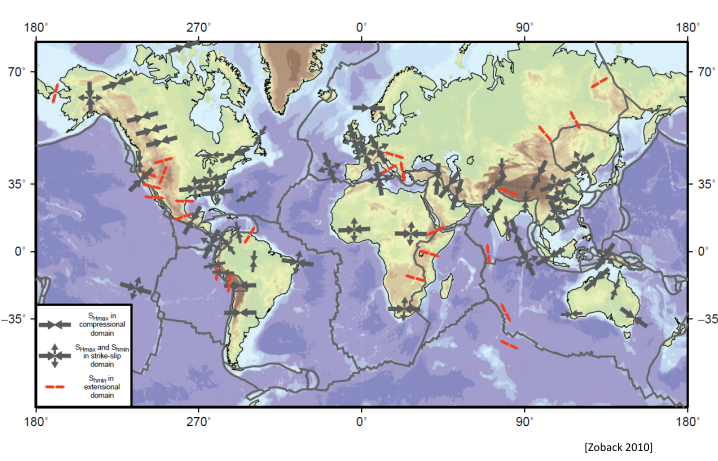
\includegraphics[scale=0.45]{.././Figures/split/1-2.pdf}%
\lthtmlpictureZ
\lthtmlcheckvsize\clearpage}

{\newpage\clearpage
\lthtmlpictureA{tex2html_wrap19792}%
\includegraphics[scale=0.50]{.././Figures/split/1-3.pdf}%
\lthtmlpictureZ
\lthtmlcheckvsize\clearpage}

\stepcounter{section}
\stepcounter{subsection}
{\newpage\clearpage
\lthtmlpictureA{tex2html_wrap19801}%
\includegraphics[scale=0.55]{.././Figures/split/1-4.pdf}%
\lthtmlpictureZ
\lthtmlcheckvsize\clearpage}

\stepcounter{subsection}
{\newpage\clearpage
\lthtmlpictureA{tex2html_wrap19809}%
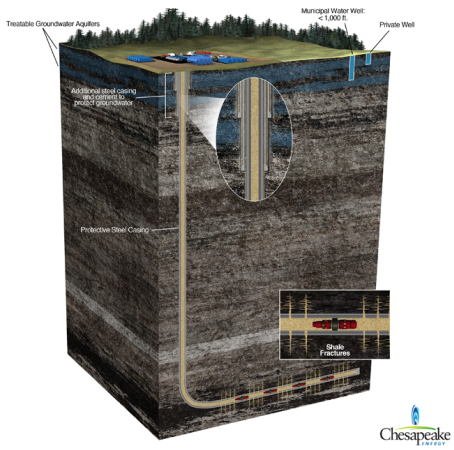
\includegraphics[scale=0.65]{.././Figures/split/1-6.pdf}%
\lthtmlpictureZ
\lthtmlcheckvsize\clearpage}

\stepcounter{subsection}
{\newpage\clearpage
\lthtmlpictureA{tex2html_wrap19815}%
\includegraphics[scale=0.50]{.././Figures/split/1-5.pdf}%
\lthtmlpictureZ
\lthtmlcheckvsize\clearpage}

\stepcounter{section}
\stepcounter{chapter}
\stepcounter{section}
\stepcounter{subsection}
{\newpage\clearpage
\lthtmlinlinemathA{tex2html_wrap_inline19826}%
$ \uline{F}_1$%
\lthtmlindisplaymathZ
\lthtmlcheckvsize\clearpage}

{\newpage\clearpage
\lthtmlinlinemathA{tex2html_wrap_inline19828}%
$ \uline{F}_2$%
\lthtmlindisplaymathZ
\lthtmlcheckvsize\clearpage}

{\newpage\clearpage
\lthtmlinlinemathA{tex2html_wrap_inline19830}%
$ {\rm I\!R}^3$%
\lthtmlindisplaymathZ
\lthtmlcheckvsize\clearpage}

{\newpage\clearpage
\lthtmlinlinemathA{tex2html_wrap_inline19832}%
$ \uline{F}_1 = \uline{F}_2$%
\lthtmlindisplaymathZ
\lthtmlcheckvsize\clearpage}

{\newpage\clearpage
\lthtmlinlinemathA{tex2html_wrap_inline19834}%
$ \uline{F}_1 =  \uline{F}_2 + m \uline{g}$%
\lthtmlindisplaymathZ
\lthtmlcheckvsize\clearpage}

{\newpage\clearpage
\lthtmlinlinemathA{tex2html_wrap_inline19836}%
$ m \uline{g}$%
\lthtmlindisplaymathZ
\lthtmlcheckvsize\clearpage}

{\newpage\clearpage
\lthtmlinlinemathA{tex2html_wrap_inline19838}%
$ \uline{F}$%
\lthtmlindisplaymathZ
\lthtmlcheckvsize\clearpage}

{\newpage\clearpage
\lthtmlinlinemathA{tex2html_wrap_inline19840}%
$ A$%
\lthtmlindisplaymathZ
\lthtmlcheckvsize\clearpage}

{\newpage\clearpage
\lthtmlinlinemathA{tex2html_wrap_indisplay19842}%
$\displaystyle \uline{\sigma} = \frac{\uline{F}}{A}$%
\lthtmlindisplaymathZ
\lthtmlcheckvsize\clearpage}

{\newpage\clearpage
\lthtmlpictureA{tex2html_wrap19844}%
\includegraphics[scale=0.50]{.././Figures/split/2-2.pdf}%
\lthtmlpictureZ
\lthtmlcheckvsize\clearpage}

\stepcounter{subsection}
{\newpage\clearpage
\lthtmlinlinemathA{tex2html_wrap_inline19850}%
$ \Delta x \Delta y \Delta x$%
\lthtmlindisplaymathZ
\lthtmlcheckvsize\clearpage}

{\newpage\clearpage
\lthtmlinlinemathA{tex2html_wrap_inline19852}%
$ \sum \uline{F} = 0$%
\lthtmlindisplaymathZ
\lthtmlcheckvsize\clearpage}

{\newpage\clearpage
\lthtmlinlinemathA{tex2html_wrap_inline19854}%
$ \uline{g}$%
\lthtmlindisplaymathZ
\lthtmlcheckvsize\clearpage}

{\newpage\clearpage
\lthtmlinlinemathA{tex2html_wrap_inline19856}%
$ \sum F_z = 0$%
\lthtmlindisplaymathZ
\lthtmlcheckvsize\clearpage}

{\newpage\clearpage
\lthtmlinlinemathA{tex2html_wrap_indisplay19859}%
$\displaystyle S_v A + \rho_{bulk} Vol  g = S_v A + \Delta S_v A$%
\lthtmlindisplaymathZ
\lthtmlcheckvsize\clearpage}

{\newpage\clearpage
\lthtmlinlinemathA{tex2html_wrap_indisplay19861}%
$\displaystyle \rho_{bulk} \: \Delta x \Delta y \Delta z \:  g = \Delta S_v \Delta x \Delta y$%
\lthtmlindisplaymathZ
\lthtmlcheckvsize\clearpage}

{\newpage\clearpage
\lthtmlinlinemathA{tex2html_wrap_indisplay19863}%
$\displaystyle \frac{\Delta S_v}{\Delta z} = \rho_{bulk} \: g$%
\lthtmlindisplaymathZ
\lthtmlcheckvsize\clearpage}

{\newpage\clearpage
\lthtmlpictureA{tex2html_wrap19865}%
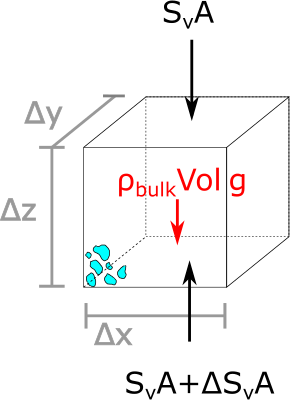
\includegraphics[scale=0.40]{.././Figures/split/2-REVoverburden.pdf}%
\lthtmlpictureZ
\lthtmlcheckvsize\clearpage}

{\newpage\clearpage
\lthtmlinlinemathA{tex2html_wrap_indisplay19870}%
$\displaystyle \int_0^{S_v(z)} dS_v = \int_0^z \rho_{bulk}(z) g \: dz$%
\lthtmlindisplaymathZ
\lthtmlcheckvsize\clearpage}

{\newpage\clearpage
\lthtmlinlinemathA{tex2html_wrap_inline19872}%
$ \rho_{bulk}(z) g$%
\lthtmlindisplaymathZ
\lthtmlcheckvsize\clearpage}

{\newpage\clearpage
\lthtmlinlinemathA{tex2html_wrap_inline19874}%
$ S_v(z=0)=0$%
\lthtmlindisplaymathZ
\lthtmlcheckvsize\clearpage}

{\newpage\clearpage
\lthtmlinlinemathA{tex2html_wrap_inline19876}%
$ \rho_{bulk} = cst$%
\lthtmlindisplaymathZ
\lthtmlcheckvsize\clearpage}

{\newpage\clearpage
\lthtmlinlinemathA{tex2html_wrap_inline19880}%
$ z$%
\lthtmlindisplaymathZ
\lthtmlcheckvsize\clearpage}

{\newpage\clearpage
\lthtmlinlinemathA{tex2html_wrap_indisplay19882}%
$\displaystyle S_v(z)  = \rho_{bulk} g \:z .$%
\lthtmlindisplaymathZ
\lthtmlcheckvsize\clearpage}

{\newpage\clearpage
\lthtmlinlinemathA{tex2html_wrap_inline19884}%
$ \rho_{SiO_2}$%
\lthtmlindisplaymathZ
\lthtmlcheckvsize\clearpage}

{\newpage\clearpage
\lthtmlinlinemathA{tex2html_wrap_inline19886}%
$ \rho_w$%
\lthtmlindisplaymathZ
\lthtmlcheckvsize\clearpage}

{\newpage\clearpage
\lthtmlinlinemathA{tex2html_wrap_inline19888}%
$ \rho_{bulk}$%
\lthtmlindisplaymathZ
\lthtmlcheckvsize\clearpage}

{\newpage\clearpage
\lthtmlinlinemathA{tex2html_wrap_inline19890}%
$ \phi$%
\lthtmlindisplaymathZ
\lthtmlcheckvsize\clearpage}

{\newpage\clearpage
\lthtmlinlinemathA{tex2html_wrap_indisplay19892}%
$\displaystyle \rho_{bulk} = (1-\phi) \rho_{SiO_2} + \phi \rho_w$%
\lthtmlindisplaymathZ
\lthtmlcheckvsize\clearpage}

{\newpage\clearpage
\lthtmlinlinemathA{tex2html_wrap_inline19894}%
$ \rho_{SiO_2} = 2650$%
\lthtmlindisplaymathZ
\lthtmlcheckvsize\clearpage}

{\newpage\clearpage
\lthtmlinlinemathA{tex2html_wrap_inline19896}%
$ ^3$%
\lthtmlindisplaymathZ
\lthtmlcheckvsize\clearpage}

{\newpage\clearpage
\lthtmlinlinemathA{tex2html_wrap_inline19898}%
$ \rho_w = 1000$%
\lthtmlindisplaymathZ
\lthtmlcheckvsize\clearpage}

{\newpage\clearpage
\lthtmlinlinemathA{tex2html_wrap_indisplay19902}%
$\displaystyle \rho_{bulk} = (1-0.2) \times 2650$%
\lthtmlindisplaymathZ
\lthtmlcheckvsize\clearpage}

{\newpage\clearpage
\lthtmlinlinemathA{tex2html_wrap_indisplay19903}%
$\displaystyle ^3 + (0.2) \times 1000$%
\lthtmlindisplaymathZ
\lthtmlcheckvsize\clearpage}

{\newpage\clearpage
\lthtmlinlinemathA{tex2html_wrap_indisplay19904}%
$\displaystyle ^3 = 2320$%
\lthtmlindisplaymathZ
\lthtmlcheckvsize\clearpage}

{\newpage\clearpage
\lthtmlinlinemathA{tex2html_wrap_indisplay19905}%
$\displaystyle ^3 .$%
\lthtmlindisplaymathZ
\lthtmlcheckvsize\clearpage}

{\newpage\clearpage
\lthtmlinlinemathA{tex2html_wrap_indisplay19911}%
$\displaystyle \rho_{bulk} \: g = 2320$%
\lthtmlindisplaymathZ
\lthtmlcheckvsize\clearpage}

{\newpage\clearpage
\lthtmlinlinemathA{tex2html_wrap_indisplay19912}%
$\displaystyle ^3 \times 9.8$%
\lthtmlindisplaymathZ
\lthtmlcheckvsize\clearpage}

{\newpage\clearpage
\lthtmlinlinemathA{tex2html_wrap_indisplay19913}%
$\displaystyle ^2 = 22.7 \times 10^3$%
\lthtmlindisplaymathZ
\lthtmlcheckvsize\clearpage}

{\newpage\clearpage
\lthtmlinlinemathA{tex2html_wrap_indisplay19914}%
$\displaystyle = 22.7$%
\lthtmlindisplaymathZ
\lthtmlcheckvsize\clearpage}

{\newpage\clearpage
\lthtmlinlinemathA{tex2html_wrap_indisplay19915}%
$\displaystyle .$%
\lthtmlindisplaymathZ
\lthtmlcheckvsize\clearpage}

{\newpage\clearpage
\lthtmlinlinemathA{tex2html_wrap_inline19917}%
$ ^2$%
\lthtmlindisplaymathZ
\lthtmlcheckvsize\clearpage}

{\newpage\clearpage
\lthtmlinlinemathA{tex2html_wrap_inline19921}%
$ ^6$%
\lthtmlindisplaymathZ
\lthtmlcheckvsize\clearpage}

{\newpage\clearpage
\lthtmlinlinemathA{tex2html_wrap_inline19925}%
$ g$%
\lthtmlindisplaymathZ
\lthtmlcheckvsize\clearpage}

{\newpage\clearpage
\lthtmlinlinemathA{tex2html_wrap_indisplay19931}%
$\displaystyle \rho_{bulk} g = 144.8$%
\lthtmlindisplaymathZ
\lthtmlcheckvsize\clearpage}

{\newpage\clearpage
\lthtmlinlinemathA{tex2html_wrap_indisplay19932}%
$\displaystyle ^3
= 144.8$%
\lthtmlindisplaymathZ
\lthtmlcheckvsize\clearpage}

{\newpage\clearpage
\lthtmlinlinemathA{tex2html_wrap_indisplay19933}%
$\displaystyle ^2 \times$%
\lthtmlindisplaymathZ
\lthtmlcheckvsize\clearpage}

{\newpage\clearpage
\lthtmlinlinemathA{tex2html_wrap_indisplay19934}%
$\displaystyle = 144.8$%
\lthtmlindisplaymathZ
\lthtmlcheckvsize\clearpage}

{\newpage\clearpage
\lthtmlinlinemathA{tex2html_wrap_indisplay19936}%
$\displaystyle = 1.01$%
\lthtmlindisplaymathZ
\lthtmlcheckvsize\clearpage}

{\newpage\clearpage
\lthtmlinlinemathA{tex2html_wrap_indisplay19937}%
$\displaystyle . \: \: \blacksquare$%
\lthtmlindisplaymathZ
\lthtmlcheckvsize\clearpage}

{\newpage\clearpage
\lthtmlinlinemathA{tex2html_wrap_inline19939}%
$ \sim 1$%
\lthtmlindisplaymathZ
\lthtmlcheckvsize\clearpage}

{\newpage\clearpage
\lthtmlinlinemathA{tex2html_wrap_inline19941}%
$ \sim 23$%
\lthtmlindisplaymathZ
\lthtmlcheckvsize\clearpage}

{\newpage\clearpage
\lthtmlinlinemathA{tex2html_wrap_inline19943}%
$ \phi = 0.20$%
\lthtmlindisplaymathZ
\lthtmlcheckvsize\clearpage}

{\newpage\clearpage
\lthtmlinlinemathA{tex2html_wrap_inline19945}%
$ \sim 0.44$%
\lthtmlindisplaymathZ
\lthtmlcheckvsize\clearpage}

{\newpage\clearpage
\lthtmlinlinemathA{tex2html_wrap_inline19947}%
$ \sim 10$%
\lthtmlindisplaymathZ
\lthtmlcheckvsize\clearpage}

{\newpage\clearpage
\lthtmlinlinemathA{tex2html_wrap_inline19949}%
$ S_w, S_o, S_g$%
\lthtmlindisplaymathZ
\lthtmlcheckvsize\clearpage}

\stepcounter{subsubsection}
{\newpage\clearpage
\lthtmlinlinemathA{tex2html_wrap_indisplay19958}%
$\displaystyle P_p = \rho_w g \, z$%
\lthtmlindisplaymathZ
\lthtmlcheckvsize\clearpage}

{\newpage\clearpage
\lthtmlpictureA{tex2html_wrap19970}%
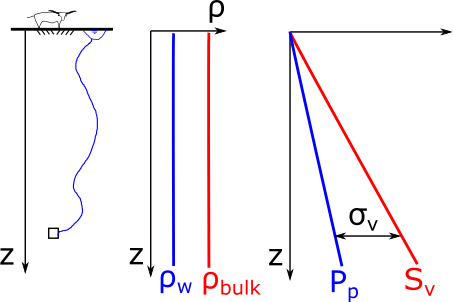
\includegraphics[scale=0.55]{.././Figures/split/2-OnshorePpSv.pdf}%
\lthtmlpictureZ
\lthtmlcheckvsize\clearpage}

{\newpage\clearpage
\lthtmlinlinemathA{tex2html_wrap_indisplay19987}%
$\displaystyle \sigma_v = S_v - P_p$%
\lthtmlindisplaymathZ
\lthtmlcheckvsize\clearpage}

{\newpage\clearpage
\lthtmlinlinemathA{tex2html_wrap_inline19989}%
$ S_v > P_p$%
\lthtmlindisplaymathZ
\lthtmlcheckvsize\clearpage}

{\newpage\clearpage
\lthtmlpictureA{tex2html_wrap19991}%
\includegraphics[scale=0.55]{.././Figures/split/2-20.pdf}%
\lthtmlpictureZ
\lthtmlcheckvsize\clearpage}

{\newpage\clearpage
\lthtmlinlinemathA{tex2html_wrap_inline19996}%
$ P_w$%
\lthtmlindisplaymathZ
\lthtmlcheckvsize\clearpage}

{\newpage\clearpage
\lthtmlinlinemathA{tex2html_wrap_indisplay20012}%
$\displaystyle \frac{dP_p}{dz} = \rho_w g = 1040$%
\lthtmlindisplaymathZ
\lthtmlcheckvsize\clearpage}

{\newpage\clearpage
\lthtmlinlinemathA{tex2html_wrap_indisplay20014}%
$\displaystyle ^2 = 10.19$%
\lthtmlindisplaymathZ
\lthtmlcheckvsize\clearpage}

{\newpage\clearpage
\lthtmlinlinemathA{tex2html_wrap_indisplay20016}%
$\displaystyle \frac{dS_v}{dz} = \rho_{bulk} g = 2350$%
\lthtmlindisplaymathZ
\lthtmlcheckvsize\clearpage}

{\newpage\clearpage
\lthtmlinlinemathA{tex2html_wrap_indisplay20018}%
$\displaystyle ^2 = 23.03$%
\lthtmlindisplaymathZ
\lthtmlcheckvsize\clearpage}

{\newpage\clearpage
\lthtmlinlinemathA{tex2html_wrap_indisplay20020}%
$\displaystyle P_p = \frac{dP_p}{dz} z = 10.19$%
\lthtmlindisplaymathZ
\lthtmlcheckvsize\clearpage}

{\newpage\clearpage
\lthtmlinlinemathA{tex2html_wrap_indisplay20021}%
$\displaystyle \times 1.219$%
\lthtmlindisplaymathZ
\lthtmlcheckvsize\clearpage}

{\newpage\clearpage
\lthtmlinlinemathA{tex2html_wrap_indisplay20022}%
$\displaystyle =  12.43$%
\lthtmlindisplaymathZ
\lthtmlcheckvsize\clearpage}

{\newpage\clearpage
\lthtmlinlinemathA{tex2html_wrap_indisplay20023}%
$\displaystyle = 1801$%
\lthtmlindisplaymathZ
\lthtmlcheckvsize\clearpage}

{\newpage\clearpage
\lthtmlinlinemathA{tex2html_wrap_indisplay20025}%
$\displaystyle \frac{dS_v}{dz} z = 23.03$%
\lthtmlindisplaymathZ
\lthtmlcheckvsize\clearpage}

{\newpage\clearpage
\lthtmlinlinemathA{tex2html_wrap_indisplay20027}%
$\displaystyle =  28.07$%
\lthtmlindisplaymathZ
\lthtmlcheckvsize\clearpage}

{\newpage\clearpage
\lthtmlinlinemathA{tex2html_wrap_indisplay20028}%
$\displaystyle = 4070$%
\lthtmlindisplaymathZ
\lthtmlcheckvsize\clearpage}

{\newpage\clearpage
\lthtmlinlinemathA{tex2html_wrap_inline20031}%
$ \: \: \blacksquare$%
\lthtmlindisplaymathZ
\lthtmlcheckvsize\clearpage}

\stepcounter{subsubsection}
{\newpage\clearpage
\lthtmlinlinemathA{tex2html_wrap_inline20034}%
$ z_w$%
\lthtmlindisplaymathZ
\lthtmlcheckvsize\clearpage}

{\newpage\clearpage
\lthtmlinlinemathA{tex2html_wrap_inline20038}%
$ z > z_w$%
\lthtmlindisplaymathZ
\lthtmlcheckvsize\clearpage}

{\newpage\clearpage
\lthtmlinlinemathA{tex2html_wrap_indisplay20040}%
$\displaystyle S_v = \rho_{w} g \, z_w + \rho_{bulk} g (z-z_w)$%
\lthtmlindisplaymathZ
\lthtmlcheckvsize\clearpage}

{\newpage\clearpage
\lthtmlinlinemathA{tex2html_wrap_indisplay20041}%
$\displaystyle \quad z \geq z_w$%
\lthtmlindisplaymathZ
\lthtmlcheckvsize\clearpage}

{\newpage\clearpage
\lthtmlpictureA{tex2html_wrap20043}%
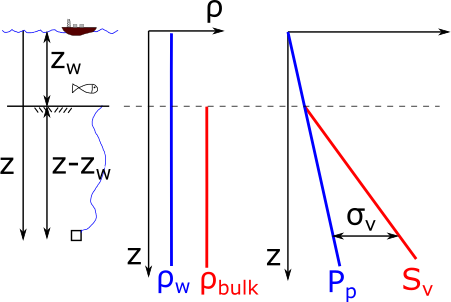
\includegraphics[scale=0.55]{.././Figures/split/2-OffshorePpSv.pdf}%
\lthtmlpictureZ
\lthtmlcheckvsize\clearpage}

{\newpage\clearpage
\lthtmlinlinemathA{tex2html_wrap_inline20048}%
$ z=z_w$%
\lthtmlindisplaymathZ
\lthtmlcheckvsize\clearpage}

{\newpage\clearpage
\lthtmlinlinemathA{tex2html_wrap_indisplay20050}%
$\displaystyle \sigma_v = S_v - P_p =  \rho_{bulk} g (z-z_w)$%
\lthtmlindisplaymathZ
\lthtmlcheckvsize\clearpage}

{\newpage\clearpage
\lthtmlinlinemathA{tex2html_wrap_indisplay20057}%
$\displaystyle P_p = \rho_w g z_w + \frac{dP_p}{dz} (z-z_w)  = 0.44$%
\lthtmlindisplaymathZ
\lthtmlcheckvsize\clearpage}

{\newpage\clearpage
\lthtmlinlinemathA{tex2html_wrap_indisplay20058}%
$\displaystyle \times 2000$%
\lthtmlindisplaymathZ
\lthtmlcheckvsize\clearpage}

{\newpage\clearpage
\lthtmlinlinemathA{tex2html_wrap_indisplay20059}%
$\displaystyle + 0.44$%
\lthtmlindisplaymathZ
\lthtmlcheckvsize\clearpage}

{\newpage\clearpage
\lthtmlinlinemathA{tex2html_wrap_indisplay20060}%
$\displaystyle \times (9000-2000)$%
\lthtmlindisplaymathZ
\lthtmlcheckvsize\clearpage}

{\newpage\clearpage
\lthtmlinlinemathA{tex2html_wrap_indisplay20061}%
$\displaystyle =   3960$%
\lthtmlindisplaymathZ
\lthtmlcheckvsize\clearpage}

{\newpage\clearpage
\lthtmlinlinemathA{tex2html_wrap_indisplay20063}%
$\displaystyle S_v = \rho_w g z_w + \frac{dS_v}{dz} (z-z_w)  = 0.44$%
\lthtmlindisplaymathZ
\lthtmlcheckvsize\clearpage}

{\newpage\clearpage
\lthtmlinlinemathA{tex2html_wrap_indisplay20065}%
$\displaystyle + 1.00$%
\lthtmlindisplaymathZ
\lthtmlcheckvsize\clearpage}

{\newpage\clearpage
\lthtmlinlinemathA{tex2html_wrap_indisplay20067}%
$\displaystyle = 7880$%
\lthtmlindisplaymathZ
\lthtmlcheckvsize\clearpage}

{\newpage\clearpage
\lthtmlinlinemathA{tex2html_wrap_indisplay20068}%
$\displaystyle ,$%
\lthtmlindisplaymathZ
\lthtmlcheckvsize\clearpage}

{\newpage\clearpage
\lthtmlinlinemathA{tex2html_wrap_indisplay20070}%
$\displaystyle \sigma_v = S_v - P_p = 7880$%
\lthtmlindisplaymathZ
\lthtmlcheckvsize\clearpage}

{\newpage\clearpage
\lthtmlinlinemathA{tex2html_wrap_indisplay20071}%
$\displaystyle - 3960$%
\lthtmlindisplaymathZ
\lthtmlcheckvsize\clearpage}

{\newpage\clearpage
\lthtmlinlinemathA{tex2html_wrap_indisplay20072}%
$\displaystyle = 3920$%
\lthtmlindisplaymathZ
\lthtmlcheckvsize\clearpage}

{\newpage\clearpage
\lthtmlinlinemathA{tex2html_wrap_inline20075}%
$ P_p = 27.31$%
\lthtmlindisplaymathZ
\lthtmlcheckvsize\clearpage}

{\newpage\clearpage
\lthtmlinlinemathA{tex2html_wrap_inline20077}%
$ S_v =  54.34$%
\lthtmlindisplaymathZ
\lthtmlcheckvsize\clearpage}

{\newpage\clearpage
\lthtmlinlinemathA{tex2html_wrap_inline20079}%
$ \sigma_v = 27.03$%
\lthtmlindisplaymathZ
\lthtmlcheckvsize\clearpage}

\stepcounter{subsubsection}
{\newpage\clearpage
\lthtmlinlinemathA{tex2html_wrap_indisplay20086}%
$\displaystyle S_v(z) = \int_0^z \rho_{bulk}(z) g \: dz$%
\lthtmlindisplaymathZ
\lthtmlcheckvsize\clearpage}

{\newpage\clearpage
\lthtmlinlinemathA{tex2html_wrap_inline20088}%
$ \rho_{bulk}(z)$%
\lthtmlindisplaymathZ
\lthtmlcheckvsize\clearpage}

{\newpage\clearpage
\lthtmlinlinemathA{tex2html_wrap_indisplay20096}%
$\displaystyle S_v(z_i) = \sum\limits_1^i \rho_{bulk}(z_i) g \Delta z_i$%
\lthtmlindisplaymathZ
\lthtmlcheckvsize\clearpage}

{\newpage\clearpage
\lthtmlinlinemathA{tex2html_wrap_inline20098}%
$ i$%
\lthtmlindisplaymathZ
\lthtmlcheckvsize\clearpage}

{\newpage\clearpage
\lthtmlinlinemathA{tex2html_wrap_inline20100}%
$ z_i$%
\lthtmlindisplaymathZ
\lthtmlcheckvsize\clearpage}

{\newpage\clearpage
\lthtmlpictureA{tex2html_wrap20104}%
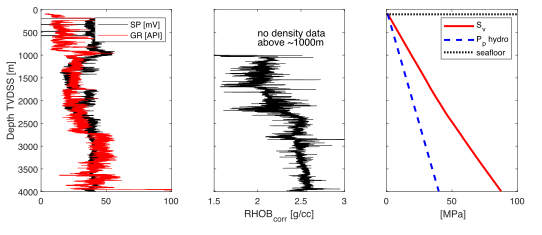
\includegraphics[scale=0.85]{.././Figures/split/2-VertStress_TVDSS.pdf}%
\lthtmlpictureZ
\lthtmlcheckvsize\clearpage}

\stepcounter{section}
{\newpage\clearpage
\lthtmlinlinemathA{tex2html_wrap_inline20110}%
$ z \sim 8,500$%
\lthtmlindisplaymathZ
\lthtmlcheckvsize\clearpage}

{\newpage\clearpage
\lthtmlinlinemathA{tex2html_wrap_inline20114}%
$ z \sim 11,000$%
\lthtmlindisplaymathZ
\lthtmlcheckvsize\clearpage}

{\newpage\clearpage
\lthtmlpictureA{tex2html_wrap20118}%
\includegraphics[scale=0.65]{.././Figures/split/2-9.pdf}%
\lthtmlpictureZ
\lthtmlcheckvsize\clearpage}

{\newpage\clearpage
\lthtmlinlinemathA{tex2html_wrap_inline20123}%
$ \lambda_p$%
\lthtmlindisplaymathZ
\lthtmlcheckvsize\clearpage}

{\newpage\clearpage
\lthtmlinlinemathA{tex2html_wrap_indisplay20125}%
$\displaystyle \lambda_p(z) = \frac{P_p(z)}{S_v(z)}$%
\lthtmlindisplaymathZ
\lthtmlcheckvsize\clearpage}

{\newpage\clearpage
\lthtmlinlinemathA{tex2html_wrap_inline20131}%
$ \lambda_p \leq 1$%
\lthtmlindisplaymathZ
\lthtmlcheckvsize\clearpage}

{\newpage\clearpage
\lthtmlinlinemathA{tex2html_wrap_inline20133}%
$ \lambda_p \sim 0.44$%
\lthtmlindisplaymathZ
\lthtmlcheckvsize\clearpage}

{\newpage\clearpage
\lthtmlinlinemathA{tex2html_wrap_inline20135}%
$ \lambda_p \neq 0.44$%
\lthtmlindisplaymathZ
\lthtmlcheckvsize\clearpage}

{\newpage\clearpage
\lthtmlinlinemathA{tex2html_wrap_inline20137}%
$ \lambda_p \rightarrow 1$%
\lthtmlindisplaymathZ
\lthtmlcheckvsize\clearpage}

\stepcounter{subsection}
{\newpage\clearpage
\lthtmlinlinemathA{tex2html_wrap_inline20140}%
$ P_p > P_p^{\text{hydrostatic}}$%
\lthtmlindisplaymathZ
\lthtmlcheckvsize\clearpage}

{\newpage\clearpage
\lthtmlinlinemathA{tex2html_wrap_inline20142}%
$ \Delta P_p$%
\lthtmlindisplaymathZ
\lthtmlcheckvsize\clearpage}

{\newpage\clearpage
\lthtmlinlinemathA{tex2html_wrap_inline20144}%
$ h$%
\lthtmlindisplaymathZ
\lthtmlcheckvsize\clearpage}

{\newpage\clearpage
\lthtmlinlinemathA{tex2html_wrap_inline20146}%
$ \rho_{brine} - \rho_{hydrocarbon}$%
\lthtmlindisplaymathZ
\lthtmlcheckvsize\clearpage}

{\newpage\clearpage
\lthtmlinlinemathA{tex2html_wrap_indisplay20148}%
$\displaystyle \Delta P = (\rho_{brine} - \rho_{hydrocarbon}) g  h$%
\lthtmlindisplaymathZ
\lthtmlcheckvsize\clearpage}

{\newpage\clearpage
\lthtmlpictureA{tex2html_wrap20156}%
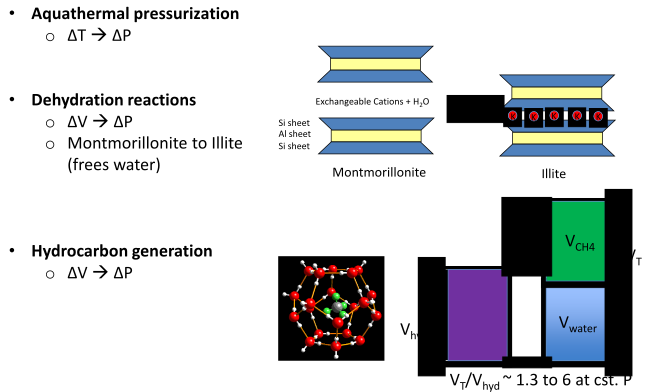
\includegraphics[scale=0.50]{.././Figures/split/2-11.pdf}%
\lthtmlpictureZ
\lthtmlcheckvsize\clearpage}

\stepcounter{subsection}
{\newpage\clearpage
\lthtmlinlinemathA{tex2html_wrap_inline20162}%
$ W$%
\lthtmlindisplaymathZ
\lthtmlcheckvsize\clearpage}

{\newpage\clearpage
\lthtmlinlinemathA{tex2html_wrap_inline20164}%
$ \Delta P = W/A$%
\lthtmlindisplaymathZ
\lthtmlcheckvsize\clearpage}

{\newpage\clearpage
\lthtmlinlinemathA{tex2html_wrap_inline20172}%
$ \sigma_v = W/A$%
\lthtmlindisplaymathZ
\lthtmlcheckvsize\clearpage}

{\newpage\clearpage
\lthtmlinlinemathA{tex2html_wrap_inline20176}%
$ \Delta P = 0$%
\lthtmlindisplaymathZ
\lthtmlcheckvsize\clearpage}

{\newpage\clearpage
\lthtmlpictureA{tex2html_wrap20180}%
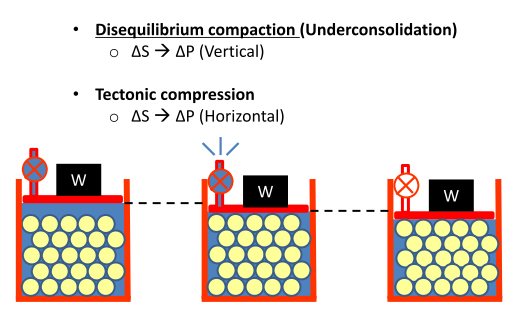
\includegraphics[scale=0.50]{.././Figures/split/2-12.pdf}%
\lthtmlpictureZ
\lthtmlcheckvsize\clearpage}

{\newpage\clearpage
\lthtmlpictureA{tex2html_wrap20185}%
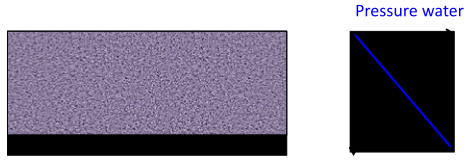
\includegraphics[scale=0.60]{.././Figures/split/2-13.pdf}%
\lthtmlpictureZ
\lthtmlcheckvsize\clearpage}

{\newpage\clearpage
\lthtmlinlinemathA{tex2html_wrap_inline20190}%
$ \Delta z$%
\lthtmlindisplaymathZ
\lthtmlcheckvsize\clearpage}

{\newpage\clearpage
\lthtmlinlinemathA{tex2html_wrap_indisplay20192}%
$\displaystyle D_h = \frac{M k} {\mu}$%
\lthtmlindisplaymathZ
\lthtmlcheckvsize\clearpage}

{\newpage\clearpage
\lthtmlinlinemathA{tex2html_wrap_inline20196}%
$ C_{bp}$%
\lthtmlindisplaymathZ
\lthtmlcheckvsize\clearpage}

{\newpage\clearpage
\lthtmlinlinemathA{tex2html_wrap_inline20198}%
$ k$%
\lthtmlindisplaymathZ
\lthtmlcheckvsize\clearpage}

{\newpage\clearpage
\lthtmlinlinemathA{tex2html_wrap_inline20200}%
$ \mu$%
\lthtmlindisplaymathZ
\lthtmlcheckvsize\clearpage}

{\newpage\clearpage
\lthtmlinlinemathA{tex2html_wrap_indisplay20202}%
$\displaystyle \frac{\partial P_p}{\partial t} = D_h \frac{d^2P_p}{dz^2}$%
\lthtmlindisplaymathZ
\lthtmlcheckvsize\clearpage}

{\newpage\clearpage
\lthtmlpictureA{tex2html_wrap20204}%
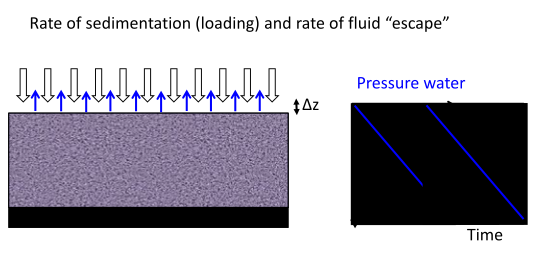
\includegraphics[scale=0.60]{.././Figures/split/2-14.pdf}%
\lthtmlpictureZ
\lthtmlcheckvsize\clearpage}

{\newpage\clearpage
\lthtmlinlinemathA{tex2html_wrap_inline20209}%
$ T_{ch}$%
\lthtmlindisplaymathZ
\lthtmlcheckvsize\clearpage}

{\newpage\clearpage
\lthtmlinlinemathA{tex2html_wrap_inline20211}%
$ \sim 2/3$%
\lthtmlindisplaymathZ
\lthtmlcheckvsize\clearpage}

{\newpage\clearpage
\lthtmlinlinemathA{tex2html_wrap_indisplay20213}%
$\displaystyle T_{ch} = \frac{L^2}{D_h}$%
\lthtmlindisplaymathZ
\lthtmlcheckvsize\clearpage}

{\newpage\clearpage
\lthtmlinlinemathA{tex2html_wrap_inline20215}%
$ L$%
\lthtmlindisplaymathZ
\lthtmlcheckvsize\clearpage}

{\newpage\clearpage
\lthtmlinlinemathA{tex2html_wrap_inline20219}%
$ k =$%
\lthtmlindisplaymathZ
\lthtmlcheckvsize\clearpage}

{\newpage\clearpage
\lthtmlinlinemathA{tex2html_wrap_inline20221}%
$ M =$%
\lthtmlindisplaymathZ
\lthtmlcheckvsize\clearpage}

{\newpage\clearpage
\lthtmlinlinemathA{tex2html_wrap_inline20227}%
$ T_{ch} \sim $%
\lthtmlindisplaymathZ
\lthtmlcheckvsize\clearpage}

{\newpage\clearpage
\lthtmlinlinemathA{tex2html_wrap_indisplay20235}%
$\displaystyle \phi = \phi_o \exp (-\beta \sigma_v)$%
\lthtmlindisplaymathZ
\lthtmlcheckvsize\clearpage}

{\newpage\clearpage
\lthtmlpictureA{tex2html_wrap20241}%
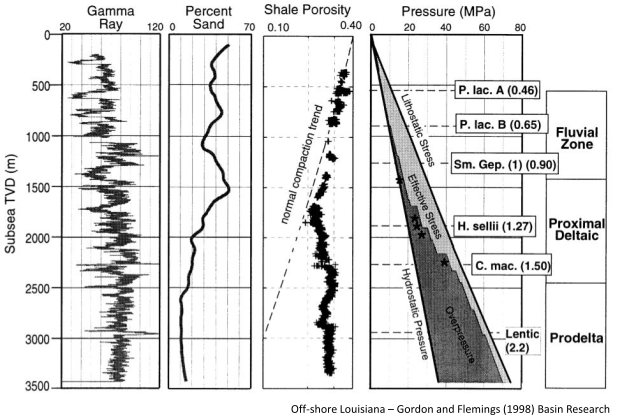
\includegraphics[scale=0.65]{.././Figures/split/2-16.pdf}%
\lthtmlpictureZ
\lthtmlcheckvsize\clearpage}

{\newpage\clearpage
\lthtmlinlinemathA{tex2html_wrap_inline20254}%
$ \phi = 0.298$%
\lthtmlindisplaymathZ
\lthtmlcheckvsize\clearpage}

{\newpage\clearpage
\lthtmlinlinemathA{tex2html_wrap_inline20256}%
$ \beta = 3.2 \times 10^{-2}$%
\lthtmlindisplaymathZ
\lthtmlcheckvsize\clearpage}

{\newpage\clearpage
\lthtmlinlinemathA{tex2html_wrap_inline20258}%
$ ^{-1}$%
\lthtmlindisplaymathZ
\lthtmlcheckvsize\clearpage}

{\newpage\clearpage
\lthtmlinlinemathA{tex2html_wrap_inline20260}%
$ \phi_0 = 0.38$%
\lthtmlindisplaymathZ
\lthtmlcheckvsize\clearpage}

{\newpage\clearpage
\lthtmlinlinemathA{tex2html_wrap_indisplay20262}%
$\displaystyle S_v = 10$%
\lthtmlindisplaymathZ
\lthtmlcheckvsize\clearpage}

{\newpage\clearpage
\lthtmlinlinemathA{tex2html_wrap_indisplay20263}%
$\displaystyle \times 0.5$%
\lthtmlindisplaymathZ
\lthtmlcheckvsize\clearpage}

{\newpage\clearpage
\lthtmlinlinemathA{tex2html_wrap_indisplay20264}%
$\displaystyle + 22$%
\lthtmlindisplaymathZ
\lthtmlcheckvsize\clearpage}

{\newpage\clearpage
\lthtmlinlinemathA{tex2html_wrap_indisplay20265}%
$\displaystyle \times 1.5$%
\lthtmlindisplaymathZ
\lthtmlcheckvsize\clearpage}

{\newpage\clearpage
\lthtmlinlinemathA{tex2html_wrap_indisplay20266}%
$\displaystyle = 38$%
\lthtmlindisplaymathZ
\lthtmlcheckvsize\clearpage}

{\newpage\clearpage
\lthtmlinlinemathA{tex2html_wrap_indisplay20269}%
$\displaystyle \sigma_v = - \frac{\ln \left( \phi / \phi_o \right)}{\beta} = 7.6$%
\lthtmlindisplaymathZ
\lthtmlcheckvsize\clearpage}

{\newpage\clearpage
\lthtmlinlinemathA{tex2html_wrap_inline20272}%
$ S_v = \sigma_v + P_p$%
\lthtmlindisplaymathZ
\lthtmlcheckvsize\clearpage}

{\newpage\clearpage
\lthtmlinlinemathA{tex2html_wrap_indisplay20274}%
$\displaystyle P_p = S_v - \sigma_v =
38$%
\lthtmlindisplaymathZ
\lthtmlcheckvsize\clearpage}

{\newpage\clearpage
\lthtmlinlinemathA{tex2html_wrap_indisplay20275}%
$\displaystyle - 7.6$%
\lthtmlindisplaymathZ
\lthtmlcheckvsize\clearpage}

{\newpage\clearpage
\lthtmlinlinemathA{tex2html_wrap_indisplay20276}%
$\displaystyle = 30.40$%
\lthtmlindisplaymathZ
\lthtmlcheckvsize\clearpage}

{\newpage\clearpage
\lthtmlinlinemathA{tex2html_wrap_indisplay20279}%
$\displaystyle \lambda_p = \frac{P_p}{S_v} = 	\frac{30.40 \text{ MPa}}{38 \text{ MPa}} = 0.8. \: \: \blacksquare$%
\lthtmlindisplaymathZ
\lthtmlcheckvsize\clearpage}

\stepcounter{subsection}
{\newpage\clearpage
\lthtmlpictureA{tex2html_wrap20282}%
\includegraphics[scale=0.65]{.././Figures/split/2-17.pdf}%
\lthtmlpictureZ
\lthtmlcheckvsize\clearpage}

\stepcounter{section}
\stepcounter{subsection}
{\newpage\clearpage
\lthtmlinlinemathA{tex2html_wrap_inline20295}%
$ S_{Hmax} \geq S_{hmin}$%
\lthtmlindisplaymathZ
\lthtmlcheckvsize\clearpage}

{\newpage\clearpage
\lthtmlpictureA{tex2html_wrap20297}%
\includegraphics[scale=0.50]{.././Figures/split/3-20.pdf}%
\lthtmlpictureZ
\lthtmlcheckvsize\clearpage}

{\newpage\clearpage
\lthtmlpictureA{tex2html_wrap20302}%
\includegraphics[scale=0.50]{.././Figures/split/3-16.pdf}%
\lthtmlpictureZ
\lthtmlcheckvsize\clearpage}

{\newpage\clearpage
\lthtmlpictureA{tex2html_wrap20307}%
\includegraphics[scale=0.55]{.././Figures/split/3-18.pdf}%
\lthtmlpictureZ
\lthtmlcheckvsize\clearpage}

\stepcounter{subsection}
{\newpage\clearpage
\lthtmlpictureA{tex2html_wrap20315}%
\includegraphics[scale=0.55]{.././Figures/split/3-2.pdf}%
\lthtmlpictureZ
\lthtmlcheckvsize\clearpage}

\stepcounter{subsection}
{\newpage\clearpage
\lthtmlinlinemathA{tex2html_wrap_inline20323}%
$ S_v > S_{hmin} = S_3$%
\lthtmlindisplaymathZ
\lthtmlcheckvsize\clearpage}

\stepcounter{subsection}
{\newpage\clearpage
\lthtmlinlinemathA{tex2html_wrap_inline20348}%
$ S_1$%
\lthtmlindisplaymathZ
\lthtmlcheckvsize\clearpage}

{\newpage\clearpage
\lthtmlinlinemathA{tex2html_wrap_inline20350}%
$ S_2$%
\lthtmlindisplaymathZ
\lthtmlcheckvsize\clearpage}

\stepcounter{subsubsection}
{\newpage\clearpage
\lthtmlinlinemathA{tex2html_wrap_inline20373}%
$ S_v > S_{Hmax} > S_{hmin}$%
\lthtmlindisplaymathZ
\lthtmlcheckvsize\clearpage}

{\newpage\clearpage
\lthtmlinlinemathA{tex2html_wrap_inline20375}%
$ S_1 = S_v$%
\lthtmlindisplaymathZ
\lthtmlcheckvsize\clearpage}

{\newpage\clearpage
\lthtmlinlinemathA{tex2html_wrap_inline20377}%
$ S_2 = S_{Hmax}$%
\lthtmlindisplaymathZ
\lthtmlcheckvsize\clearpage}

{\newpage\clearpage
\lthtmlinlinemathA{tex2html_wrap_inline20379}%
$ S_3 = S_{hmin}$%
\lthtmlindisplaymathZ
\lthtmlcheckvsize\clearpage}

{\newpage\clearpage
\lthtmlinlinemathA{tex2html_wrap_inline20383}%
$ \sim 60$%
\lthtmlindisplaymathZ
\lthtmlcheckvsize\clearpage}

{\newpage\clearpage
\lthtmlinlinemathA{tex2html_wrap_inline20387}%
$ \sigma_1 = S_1 - P_p$%
\lthtmlindisplaymathZ
\lthtmlcheckvsize\clearpage}

{\newpage\clearpage
\lthtmlinlinemathA{tex2html_wrap_inline20389}%
$ \sigma_3 = S_3 - P_p$%
\lthtmlindisplaymathZ
\lthtmlcheckvsize\clearpage}

{\newpage\clearpage
\lthtmlpictureA{tex2html_wrap20393}%
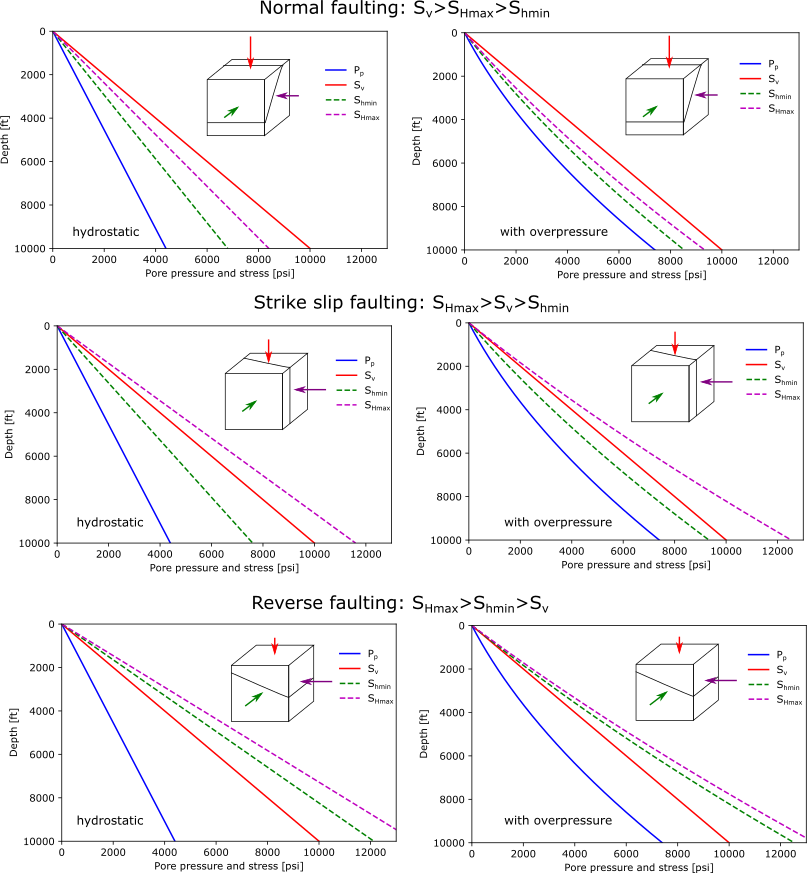
\includegraphics[scale=0.55]{.././Figures/split/2-StressProfiles.pdf}%
\lthtmlpictureZ
\lthtmlcheckvsize\clearpage}

\stepcounter{subsubsection}
{\newpage\clearpage
\lthtmlinlinemathA{tex2html_wrap_inline20399}%
$ S_{Hmax} > S_v > S_{hmin}$%
\lthtmlindisplaymathZ
\lthtmlcheckvsize\clearpage}

{\newpage\clearpage
\lthtmlinlinemathA{tex2html_wrap_inline20401}%
$ S_1 = S_{Hmax}$%
\lthtmlindisplaymathZ
\lthtmlcheckvsize\clearpage}

{\newpage\clearpage
\lthtmlinlinemathA{tex2html_wrap_inline20403}%
$ S_2 = S_v$%
\lthtmlindisplaymathZ
\lthtmlcheckvsize\clearpage}

\stepcounter{subsubsection}
{\newpage\clearpage
\lthtmlinlinemathA{tex2html_wrap_inline20414}%
$ S_{Hmax} > S_{hmin} > S_v$%
\lthtmlindisplaymathZ
\lthtmlcheckvsize\clearpage}

{\newpage\clearpage
\lthtmlinlinemathA{tex2html_wrap_inline20418}%
$ S_2 = S_{hmin}$%
\lthtmlindisplaymathZ
\lthtmlcheckvsize\clearpage}

{\newpage\clearpage
\lthtmlinlinemathA{tex2html_wrap_inline20420}%
$ S_3 = S_v$%
\lthtmlindisplaymathZ
\lthtmlcheckvsize\clearpage}

\stepcounter{subsection}
{\newpage\clearpage
\lthtmlinlinemathA{tex2html_wrap_inline20429}%
$ \rho_w g z$%
\lthtmlindisplaymathZ
\lthtmlcheckvsize\clearpage}

{\newpage\clearpage
\lthtmlinlinemathA{tex2html_wrap_inline20445}%
$ S_3 = S_{22}$%
\lthtmlindisplaymathZ
\lthtmlcheckvsize\clearpage}

{\newpage\clearpage
\lthtmlinlinemathA{tex2html_wrap_inline20447}%
$ S_3 = S_{11}$%
\lthtmlindisplaymathZ
\lthtmlcheckvsize\clearpage}

{\newpage\clearpage
\lthtmlinlinemathA{tex2html_wrap_inline20449}%
$ S_3 = S_{33}$%
\lthtmlindisplaymathZ
\lthtmlcheckvsize\clearpage}

{\newpage\clearpage
\lthtmlinlinemathA{tex2html_wrap_inline20451}%
$ S_{hmin} < S_{Hmax} < S_v$%
\lthtmlindisplaymathZ
\lthtmlcheckvsize\clearpage}

\stepcounter{section}
{\newpage\clearpage
\lthtmlinlinemathA{tex2html_wrap_inline20492}%
$ \beta = 3 \times 10^{-2}$%
\lthtmlindisplaymathZ
\lthtmlcheckvsize\clearpage}

{\newpage\clearpage
\lthtmlinlinemathA{tex2html_wrap_inline20498}%
$ [$%
\lthtmlindisplaymathZ
\lthtmlcheckvsize\clearpage}

{\newpage\clearpage
\lthtmlinlinemathA{tex2html_wrap_inline20500}%
$ ]$%
\lthtmlindisplaymathZ
\lthtmlcheckvsize\clearpage}

{\newpage\clearpage
\lthtmlinlinemathA{tex2html_wrap_inline20504}%
$ ^3]$%
\lthtmlindisplaymathZ
\lthtmlcheckvsize\clearpage}

{\newpage\clearpage
\lthtmlinlinemathA{tex2html_wrap_inline20506}%
$ [-]$%
\lthtmlindisplaymathZ
\lthtmlcheckvsize\clearpage}

\stepcounter{section}
\stepcounter{chapter}
\stepcounter{section}
{\newpage\clearpage
\lthtmlinlinemathA{tex2html_wrap_inline20583}%
$ \uline{e}_1$%
\lthtmlindisplaymathZ
\lthtmlcheckvsize\clearpage}

{\newpage\clearpage
\lthtmlinlinemathA{tex2html_wrap_inline20585}%
$ \uline{e}_2$%
\lthtmlindisplaymathZ
\lthtmlcheckvsize\clearpage}

{\newpage\clearpage
\lthtmlinlinemathA{tex2html_wrap_inline20587}%
$ \uline{e}_3$%
\lthtmlindisplaymathZ
\lthtmlcheckvsize\clearpage}

{\newpage\clearpage
\lthtmlinlinemathA{tex2html_wrap_inline20595}%
$ T$%
\lthtmlindisplaymathZ
\lthtmlcheckvsize\clearpage}

{\newpage\clearpage
\lthtmlinlinemathA{tex2html_wrap_inline20601}%
$ \uline{v}$%
\lthtmlindisplaymathZ
\lthtmlcheckvsize\clearpage}

{\newpage\clearpage
\lthtmlinlinemathA{tex2html_wrap_inline20621}%
$ S_{ij}=S_{ji}$%
\lthtmlindisplaymathZ
\lthtmlcheckvsize\clearpage}

{\newpage\clearpage
\lthtmlinlinemathA{tex2html_wrap_inline20623}%
$ i \neq j$%
\lthtmlindisplaymathZ
\lthtmlcheckvsize\clearpage}

{\newpage\clearpage
\lthtmlpictureA{tex2html_wrap20625}%
\includegraphics[scale=0.55]{.././Figures/split/4-3.pdf}%
\lthtmlpictureZ
\lthtmlcheckvsize\clearpage}

{\newpage\clearpage
\lthtmlinlinemathA{tex2html_wrap_inline20658}%
$ S_1 \geq S_2 \geq S_3$%
\lthtmlindisplaymathZ
\lthtmlcheckvsize\clearpage}

{\newpage\clearpage
\lthtmlpictureA{tex2html_wrap20662}%
\includegraphics[scale=0.55]{.././Figures/split/4-4.pdf}%
\lthtmlpictureZ
\lthtmlcheckvsize\clearpage}

\stepcounter{subsection}
{\newpage\clearpage
\lthtmlinlinemathA{tex2html_wrap_inline20668}%
$ \uline{a}$%
\lthtmlindisplaymathZ
\lthtmlcheckvsize\clearpage}

{\newpage\clearpage
\lthtmlinlinemathA{tex2html_wrap_inline20670}%
$ m \uline{a} = 0$%
\lthtmlindisplaymathZ
\lthtmlcheckvsize\clearpage}

{\newpage\clearpage
\lthtmlinlinemathA{tex2html_wrap_inline20672}%
$ \rho V b_1$%
\lthtmlindisplaymathZ
\lthtmlcheckvsize\clearpage}

{\newpage\clearpage
\lthtmlinlinemathA{tex2html_wrap_inline20674}%
$ \rho$%
\lthtmlindisplaymathZ
\lthtmlcheckvsize\clearpage}

{\newpage\clearpage
\lthtmlinlinemathA{tex2html_wrap_inline20676}%
$ V$%
\lthtmlindisplaymathZ
\lthtmlcheckvsize\clearpage}

{\newpage\clearpage
\lthtmlinlinemathA{tex2html_wrap_inline20678}%
$ b_1$%
\lthtmlindisplaymathZ
\lthtmlcheckvsize\clearpage}

{\newpage\clearpage
\lthtmldisplayA{displaymath20680}%
\begin{displaymath}\begin{array}{rcl}
\sum F_1 & = & 0 \\
\sum F_1 & =
& + S_{11} dx_2 dx_3 - \left[ S_{11} + (\frac{\partial S_{11}}{\partial x_1}) dx_1 \right] dx_2 dx_3 \\
& & + S_{21} dx_1 dx_3 - \left[ S_{21} + (\frac{\partial S_{21}}{\partial x_2}) dx_2 \right] dx_1 dx_3 \\
& & + S_{31} dx_1 dx_2 - \left[ S_{31} + (\frac{\partial S_{31}}{\partial x_3}) dx_3 \right] dx_1 dx_2 \\
& & - \rho (dx_1 dx_2 dx_3) b_1 = 0
\end{array}\end{displaymath}%
\lthtmldisplayZ
\lthtmlcheckvsize\clearpage}

{\newpage\clearpage
\lthtmlinlinemathA{tex2html_wrap_inline20682}%
$ (dx_1 dx_2 dx_3)$%
\lthtmlindisplaymathZ
\lthtmlcheckvsize\clearpage}

{\newpage\clearpage
\lthtmlinlinemathA{tex2html_wrap_indisplay20684}%
$\displaystyle \frac{\partial S_{11}}{\partial x_1} +
\frac{\partial S_{21}}{\partial x_2} +
\frac{\partial S_{31}}{\partial x_3} -
\rho b_1 = 0$%
\lthtmlindisplaymathZ
\lthtmlcheckvsize\clearpage}

{\newpage\clearpage
\lthtmlpictureA{tex2html_wrap20686}%
\includegraphics[scale=0.65]{.././Figures/split/4-5.pdf}%
\lthtmlpictureZ
\lthtmlcheckvsize\clearpage}

{\newpage\clearpage
\lthtmldisplayA{displaymath20703}%
\begin{displaymath}\displaystyle
\left\lbrace
\begin{array}{rcl}
\cfrac{\partial S_{11}}{\partial x_1} +
\cfrac{\partial S_{21}}{\partial x_2} +
\cfrac{\partial S_{31}}{\partial x_3} -
\rho b_1 & = & 0 \\
\cfrac{\partial S_{12}}{\partial x_1} +
\cfrac{\partial S_{22}}{\partial x_2} +
\cfrac{\partial S_{33}}{\partial x_3} -
\rho b_2 & = & 0 \\
\cfrac{\partial S_{13}}{\partial x_1} +
\cfrac{\partial S_{23}}{\partial x_2} +
\cfrac{\partial S_{33}}{\partial x_3} -
\rho b_3 & = & 0 \\
\end{array}
\right.\end{displaymath}%
\lthtmldisplayZ
\lthtmlcheckvsize\clearpage}

\stepcounter{subsection}
{\newpage\clearpage
\lthtmlinlinemathA{tex2html_wrap_inline20708}%
$ b_3 = g$%
\lthtmlindisplaymathZ
\lthtmlcheckvsize\clearpage}

{\newpage\clearpage
\lthtmlinlinemathA{tex2html_wrap_inline20710}%
$ \partial()/\partial x_1 = \partial()/\partial x_2 = 0$%
\lthtmlindisplaymathZ
\lthtmlcheckvsize\clearpage}

{\newpage\clearpage
\lthtmlinlinemathA{tex2html_wrap_indisplay20716}%
$\displaystyle S_{33}(x_3) = \int_0^{x_3} \rho(x_3) g \: dx_3$%
\lthtmlindisplaymathZ
\lthtmlcheckvsize\clearpage}

{\newpage\clearpage
\lthtmlpictureA{tex2html_wrap20718}%
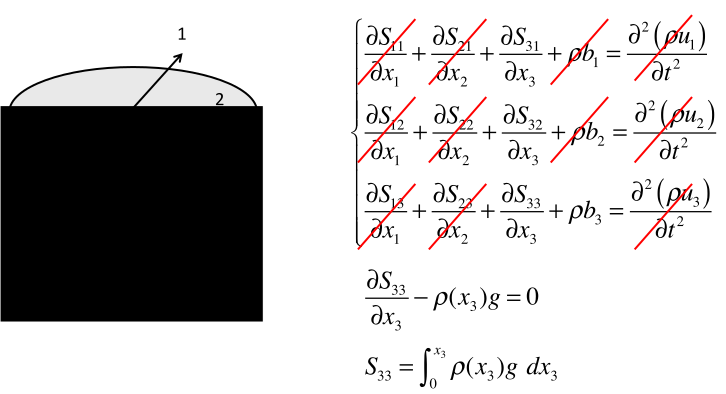
\includegraphics[scale=0.45]{.././Figures/split/4-7.pdf}%
\lthtmlpictureZ
\lthtmlcheckvsize\clearpage}

{\newpage\clearpage
\lthtmlinlinemathA{tex2html_wrap_inline20727}%
$ S_{11}$%
\lthtmlindisplaymathZ
\lthtmlcheckvsize\clearpage}

{\newpage\clearpage
\lthtmlinlinemathA{tex2html_wrap_inline20729}%
$ S_{22}$%
\lthtmlindisplaymathZ
\lthtmlcheckvsize\clearpage}

\stepcounter{subsection}
{\newpage\clearpage
\lthtmlinlinemathA{tex2html_wrap_inline20732}%
$ \uline{t}$%
\lthtmlindisplaymathZ
\lthtmlcheckvsize\clearpage}

{\newpage\clearpage
\lthtmlinlinemathA{tex2html_wrap_inline20736}%
$ \uline{b}$%
\lthtmlindisplaymathZ
\lthtmlcheckvsize\clearpage}

{\newpage\clearpage
\lthtmlpictureA{tex2html_wrap20738}%
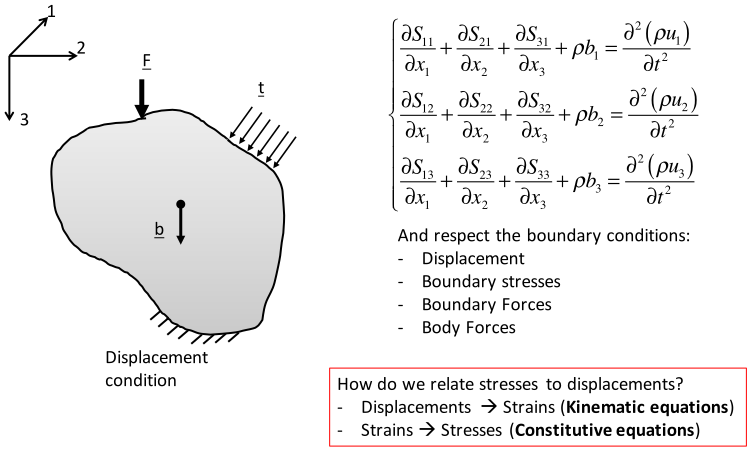
\includegraphics[scale=0.55]{.././Figures/split/4-8.pdf}%
\lthtmlpictureZ
\lthtmlcheckvsize\clearpage}

\stepcounter{section}
{\newpage\clearpage
\lthtmlpictureA{tex2html_wrap20744}%
\includegraphics[scale=0.65]{.././Figures/split/4-9.pdf}%
\lthtmlpictureZ
\lthtmlcheckvsize\clearpage}

{\newpage\clearpage
\lthtmlinlinemathA{tex2html_wrap_indisplay20751}%
$\displaystyle \varepsilon_{11} = \frac{\Delta u_1}{\Delta x_1}$%
\lthtmlindisplaymathZ
\lthtmlcheckvsize\clearpage}

{\newpage\clearpage
\lthtmlinlinemathA{tex2html_wrap_indisplay20753}%
$\displaystyle \varepsilon_{22} = \frac{\Delta u_2}{\Delta x_2}$%
\lthtmlindisplaymathZ
\lthtmlcheckvsize\clearpage}

{\newpage\clearpage
\lthtmlinlinemathA{tex2html_wrap_inline20755}%
$ \pi - \left[ \pi - \arctan(\Delta u_1 / \Delta x_2) + \arctan(\Delta u_2 / \Delta x_1) \right] $%
\lthtmlindisplaymathZ
\lthtmlcheckvsize\clearpage}

{\newpage\clearpage
\lthtmlinlinemathA{tex2html_wrap_inline20757}%
$ \arctan(x/y) \sim x/y$%
\lthtmlindisplaymathZ
\lthtmlcheckvsize\clearpage}

{\newpage\clearpage
\lthtmlinlinemathA{tex2html_wrap_indisplay20759}%
$\displaystyle \varepsilon_{12} = \frac{1}{2} \left( \frac{\Delta u_1}{\Delta x_2} + \frac{\Delta u_2}{\Delta x_1} \right)$%
\lthtmlindisplaymathZ
\lthtmlcheckvsize\clearpage}

{\newpage\clearpage
\lthtmlpictureA{tex2html_wrap20761}%
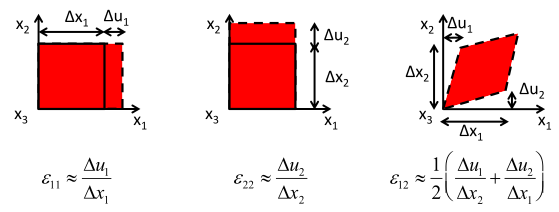
\includegraphics[scale=0.65]{.././Figures/split/4-10.pdf}%
\lthtmlpictureZ
\lthtmlcheckvsize\clearpage}

{\newpage\clearpage
\lthtmlinlinemathA{tex2html_wrap_inline20766}%
$ x_i$%
\lthtmlindisplaymathZ
\lthtmlcheckvsize\clearpage}

{\newpage\clearpage
\lthtmldisplayA{displaymath20768}%
\begin{displaymath}\uuline{\varepsilon} =
\left[
\begin{array}{ccc}
\cfrac{\partial u_1}{\partial x_1} & \cfrac{1}{2} \left( \cfrac{\partial u_1}{\partial x_2} + \cfrac{\partial u_2}{\partial x_1} \right) &  \cfrac{1}{2} \left( \cfrac{\partial u_1}{\partial x_3} + \cfrac{\partial u_3}{\partial x_1} \right)\\
\cfrac{1}{2} \left( \cfrac{\partial u_2}{\partial x_1} + \cfrac{\partial u_1}{\partial x_2} \right) & \cfrac{\partial u_2}{\partial x_2} & \cfrac{1}{2} \left( \cfrac{\partial u_2}{\partial x_3} + \cfrac{\partial u_3}{\partial x_2} \right)\\
\cfrac{1}{2} \left( \cfrac{\partial u_3}{\partial x_1} + \cfrac{\partial u_1}{\partial x_3} \right) &  \cfrac{1}{2} \left( \cfrac{\partial u_3}{\partial x_2} + \cfrac{\partial u_2}{\partial x_3} \right) & \cfrac{\partial u_3}{\partial x_3}
\end{array}
\right] =
\left[
\begin{array}{ccc}
\varepsilon_{11} & \varepsilon_{12}  &  \varepsilon_{13} \\
\varepsilon_{21} & \varepsilon_{22}  &  \varepsilon_{23} \\
\varepsilon_{31} & \varepsilon_{32}  &  \varepsilon_{33}
\end{array}
\right]\end{displaymath}%
\lthtmldisplayZ
\lthtmlcheckvsize\clearpage}

{\newpage\clearpage
\lthtmlinlinemathA{tex2html_wrap_indisplay20770}%
$\displaystyle \varepsilon_{vol} = \varepsilon_{11} + \varepsilon_{22} + \varepsilon_{33}$%
\lthtmlindisplaymathZ
\lthtmlcheckvsize\clearpage}

{\newpage\clearpage
\lthtmlinlinemathA{tex2html_wrap_inline20772}%
$ \Delta x_1 \Delta x_2 \Delta x_3$%
\lthtmlindisplaymathZ
\lthtmlcheckvsize\clearpage}

{\newpage\clearpage
\lthtmlinlinemathA{tex2html_wrap_inline20774}%
$ \Delta V$%
\lthtmlindisplaymathZ
\lthtmlcheckvsize\clearpage}

{\newpage\clearpage
\lthtmlinlinemathA{tex2html_wrap_inline20776}%
$ V_0$%
\lthtmlindisplaymathZ
\lthtmlcheckvsize\clearpage}

{\newpage\clearpage
\lthtmlinlinemathA{tex2html_wrap_indisplay20778}%
$\displaystyle \varepsilon_{vol} =  \frac{\Delta V}{V_0}
$%
\lthtmlindisplaymathZ
\lthtmlcheckvsize\clearpage}

{\newpage\clearpage
\lthtmlinlinemathA{tex2html_wrap_inline20780}%
$ \mathrm{d} x_1 \mathrm{d} x_2 \mathrm{d} x_3$%
\lthtmlindisplaymathZ
\lthtmlcheckvsize\clearpage}

{\newpage\clearpage
\lthtmlinlinemathA{tex2html_wrap_inline20782}%
$ (\mathrm{d} x_1 + \mathrm{d}u_1)(\mathrm{d} x_2 + \mathrm{d}u_2)(\mathrm{d} x_3 + \mathrm{d} u_3)$%
\lthtmlindisplaymathZ
\lthtmlcheckvsize\clearpage}

{\newpage\clearpage
\lthtmlinlinemathA{tex2html_wrap_indisplay20784}%
$\displaystyle \varepsilon_{vol} =  \frac{[(\mathrm{d} x_1 + \mathrm{d}u_1)(\mathrm{d} x_2 + \mathrm{d}u_2)(\mathrm{d} x_3 + \mathrm{d}u_3) - (\mathrm{d} x_1 \mathrm{d} x_2 \mathrm{d} x_3)]}{(\mathrm{d} x_1 \mathrm{d} x_2 \mathrm{d} x_3)}
$%
\lthtmlindisplaymathZ
\lthtmlcheckvsize\clearpage}

{\newpage\clearpage
\lthtmlinlinemathA{tex2html_wrap_inline20786}%
$ \mathrm{d}u_i \mathrm{d}u_j$%
\lthtmlindisplaymathZ
\lthtmlcheckvsize\clearpage}

{\newpage\clearpage
\lthtmlinlinemathA{tex2html_wrap_inline20788}%
$ \mathrm{d}u_1 \mathrm{d}u_2 \mathrm{d}u_3$%
\lthtmlindisplaymathZ
\lthtmlcheckvsize\clearpage}

{\newpage\clearpage
\lthtmlinlinemathA{tex2html_wrap_inline20790}%
$ \mathrm{d}u_i$%
\lthtmlindisplaymathZ
\lthtmlcheckvsize\clearpage}

{\newpage\clearpage
\lthtmlinlinemathA{tex2html_wrap_inline20792}%
$ \mathrm{d}u_i << \mathrm{d}x_j $%
\lthtmlindisplaymathZ
\lthtmlcheckvsize\clearpage}

{\newpage\clearpage
\lthtmlinlinemathA{tex2html_wrap_indisplay20794}%
$\displaystyle \varepsilon_{vol} \sim  \frac{(\mathrm{d} x_1 \mathrm{d} x_2 \mathrm{d}u_3 + 
							 \mathrm{d} x_1 \mathrm{d} x_3 \mathrm{d}u_2 +
							 \mathrm{d} x_2 \mathrm{d} x_3 \mathrm{d}u_1)}
							 {(\mathrm{d} x_1 \mathrm{d} x_2 \mathrm{d} x_3)}
				=  \frac{\mathrm{d}u_1}{\mathrm{d} x_1} + 
				   \frac{\mathrm{d}u_2}{\mathrm{d} x_2} + 
				   \frac{\mathrm{d}u_3}{\mathrm{d} x_3} 
				= \varepsilon_{11} + \varepsilon_{22} + \varepsilon_{33} \: \: \blacksquare
$%
\lthtmlindisplaymathZ
\lthtmlcheckvsize\clearpage}

\stepcounter{section}
{\newpage\clearpage
\lthtmlpictureA{tex2html_wrap20797}%
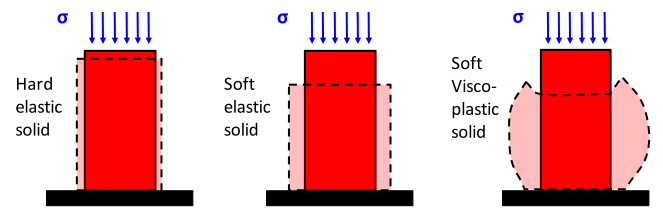
\includegraphics[scale=0.65]{.././Figures/split/4-12.pdf}%
\lthtmlpictureZ
\lthtmlcheckvsize\clearpage}

{\newpage\clearpage
\lthtmlinlinemathA{tex2html_wrap_inline20802}%
$ F$%
\lthtmlindisplaymathZ
\lthtmlcheckvsize\clearpage}

{\newpage\clearpage
\lthtmlinlinemathA{tex2html_wrap_inline20804}%
$ \Delta x$%
\lthtmlindisplaymathZ
\lthtmlcheckvsize\clearpage}

{\newpage\clearpage
\lthtmlinlinemathA{tex2html_wrap_indisplay20808}%
$\displaystyle F = k \Delta x$%
\lthtmlindisplaymathZ
\lthtmlcheckvsize\clearpage}

{\newpage\clearpage
\lthtmlinlinemathA{tex2html_wrap_inline20820}%
$ E$%
\lthtmlindisplaymathZ
\lthtmlcheckvsize\clearpage}

{\newpage\clearpage
\lthtmlinlinemathA{tex2html_wrap_indisplay20822}%
$\displaystyle \frac{F}{A} = E \frac{\Delta x}{L}$%
\lthtmlindisplaymathZ
\lthtmlcheckvsize\clearpage}

{\newpage\clearpage
\lthtmlinlinemathA{tex2html_wrap_inline20824}%
$ \sigma$%
\lthtmlindisplaymathZ
\lthtmlcheckvsize\clearpage}

{\newpage\clearpage
\lthtmlinlinemathA{tex2html_wrap_inline20826}%
$ \varepsilon$%
\lthtmlindisplaymathZ
\lthtmlcheckvsize\clearpage}

{\newpage\clearpage
\lthtmlinlinemathA{tex2html_wrap_indisplay20828}%
$\displaystyle \sigma = E \varepsilon$%
\lthtmlindisplaymathZ
\lthtmlcheckvsize\clearpage}

{\newpage\clearpage
\lthtmlinlinemathA{tex2html_wrap_inline20830}%
$ \uuline{\sigma}$%
\lthtmlindisplaymathZ
\lthtmlcheckvsize\clearpage}

{\newpage\clearpage
\lthtmlinlinemathA{tex2html_wrap_inline20832}%
$ \uuline{\varepsilon}$%
\lthtmlindisplaymathZ
\lthtmlcheckvsize\clearpage}

{\newpage\clearpage
\lthtmlinlinemathA{tex2html_wrap_inline20834}%
$ \uuline{C}$%
\lthtmlindisplaymathZ
\lthtmlcheckvsize\clearpage}

{\newpage\clearpage
\lthtmlinlinemathA{tex2html_wrap_indisplay20836}%
$\displaystyle \uuline{\sigma} = \uuline{C} \: \uuline{\varepsilon}$%
\lthtmlindisplaymathZ
\lthtmlcheckvsize\clearpage}

{\newpage\clearpage
\lthtmlpictureA{tex2html_wrap20838}%
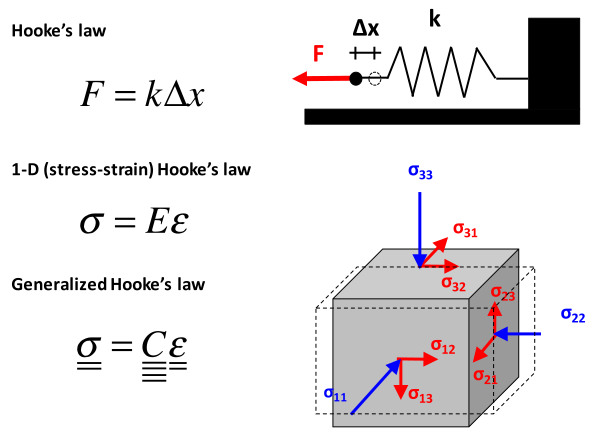
\includegraphics[scale=0.50]{.././Figures/split/4-13.pdf}%
\lthtmlpictureZ
\lthtmlcheckvsize\clearpage}

\stepcounter{subsection}
{\newpage\clearpage
\lthtmlinlinemathA{tex2html_wrap_inline20846}%
$ \sigma_{33}$%
\lthtmlindisplaymathZ
\lthtmlcheckvsize\clearpage}

{\newpage\clearpage
\lthtmlinlinemathA{tex2html_wrap_inline20852}%
$ \varepsilon_{33}$%
\lthtmlindisplaymathZ
\lthtmlcheckvsize\clearpage}

{\newpage\clearpage
\lthtmlinlinemathA{tex2html_wrap_indisplay20854}%
$\displaystyle E = \frac{\sigma_{33}}{\varepsilon_{33}}$%
\lthtmlindisplaymathZ
\lthtmlcheckvsize\clearpage}

{\newpage\clearpage
\lthtmlinlinemathA{tex2html_wrap_inline20856}%
$ \varepsilon_{11}$%
\lthtmlindisplaymathZ
\lthtmlcheckvsize\clearpage}

{\newpage\clearpage
\lthtmlinlinemathA{tex2html_wrap_inline20858}%
$ \varepsilon_{22}$%
\lthtmlindisplaymathZ
\lthtmlcheckvsize\clearpage}

{\newpage\clearpage
\lthtmlinlinemathA{tex2html_wrap_indisplay20862}%
$\displaystyle \nu = -\frac{\varepsilon_{11}}{\varepsilon_{33}}$%
\lthtmlindisplaymathZ
\lthtmlcheckvsize\clearpage}

{\newpage\clearpage
\lthtmlpictureA{tex2html_wrap20864}%
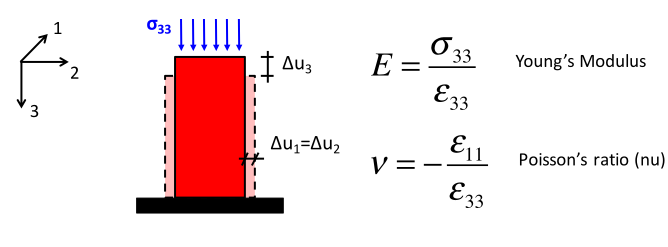
\includegraphics[scale=0.65]{.././Figures/split/4-14.pdf}%
\lthtmlpictureZ
\lthtmlcheckvsize\clearpage}

{\newpage\clearpage
\lthtmlinlinemathA{tex2html_wrap_inline20869}%
$ \sigma_a$%
\lthtmlindisplaymathZ
\lthtmlcheckvsize\clearpage}

{\newpage\clearpage
\lthtmlinlinemathA{tex2html_wrap_inline20871}%
$ \varepsilon_a$%
\lthtmlindisplaymathZ
\lthtmlcheckvsize\clearpage}

{\newpage\clearpage
\lthtmlinlinemathA{tex2html_wrap_indisplay20879}%
$\displaystyle \sigma_a = 3000$%
\lthtmlindisplaymathZ
\lthtmlcheckvsize\clearpage}

{\newpage\clearpage
\lthtmlinlinemathA{tex2html_wrap_indisplay20880}%
$\displaystyle = 3000 \frac{1}{145}$%
\lthtmlindisplaymathZ
\lthtmlcheckvsize\clearpage}

{\newpage\clearpage
\lthtmlinlinemathA{tex2html_wrap_indisplay20881}%
$\displaystyle = 20.7$%
\lthtmlindisplaymathZ
\lthtmlcheckvsize\clearpage}

{\newpage\clearpage
\lthtmlinlinemathA{tex2html_wrap_indisplay20883}%
$\displaystyle \varepsilon_a(1$%
\lthtmlindisplaymathZ
\lthtmlcheckvsize\clearpage}

{\newpage\clearpage
\lthtmlinlinemathA{tex2html_wrap_indisplay20884}%
$\displaystyle ) = \frac{\sigma_a}{E} = \frac{20.7 \text{ MPa}}{1000 \text{ MPa}} = 0.0207 = 2.07 \%
$%
\lthtmlindisplaymathZ
\lthtmlcheckvsize\clearpage}

{\newpage\clearpage
\lthtmlinlinemathA{tex2html_wrap_indisplay20886}%
$\displaystyle \varepsilon_a(10$%
\lthtmlindisplaymathZ
\lthtmlcheckvsize\clearpage}

{\newpage\clearpage
\lthtmlinlinemathA{tex2html_wrap_indisplay20887}%
$\displaystyle ) = \frac{\sigma_a}{E} = \frac{20.7 \text{ MPa}}{10000 \text{ MPa}} = 0.00207 = 0.207 \%
$%
\lthtmlindisplaymathZ
\lthtmlcheckvsize\clearpage}

{\newpage\clearpage
\lthtmlinlinemathA{tex2html_wrap_indisplay20889}%
$\displaystyle \varepsilon_a(50$%
\lthtmlindisplaymathZ
\lthtmlcheckvsize\clearpage}

{\newpage\clearpage
\lthtmlinlinemathA{tex2html_wrap_indisplay20890}%
$\displaystyle ) = \frac{\sigma_a}{E} = \frac{20.7 \text{ MPa}}{50000 \text{ MPa}} = 0.00041 = 0.041 \%
$%
\lthtmlindisplaymathZ
\lthtmlcheckvsize\clearpage}

\stepcounter{subsection}
{\newpage\clearpage
\lthtmldisplayA{displaymath20895}%
\begin{displaymath}\left\lbrace
\begin{array}{rcl}
\varepsilon_{11} & = & +\cfrac{1}{E} \: \sigma_{11} -\cfrac{\nu}{E} \: \sigma_{22} -\cfrac{\nu}{E} \: \sigma_{33}\\
\varepsilon_{22} & = &  -\cfrac{\nu}{E} \: \sigma_{11} +\cfrac{1}{E} \: \sigma_{22} - \cfrac{\nu}{E} \: \sigma_{33}\\
\varepsilon_{33} & = & -\cfrac{\nu}{E} \: \sigma_{11} -\cfrac{\nu}{E} \: \sigma_{22} + \cfrac{1}{E} \: \sigma_{33}
\end{array}
\right.\end{displaymath}%
\lthtmldisplayZ
\lthtmlcheckvsize\clearpage}

{\newpage\clearpage
\lthtmlinlinemathA{tex2html_wrap_inline20897}%
$ \varepsilon_{ij}$%
\lthtmlindisplaymathZ
\lthtmlcheckvsize\clearpage}

{\newpage\clearpage
\lthtmlinlinemathA{tex2html_wrap_inline20899}%
$ G=E/[2(1+\nu)]$%
\lthtmlindisplaymathZ
\lthtmlcheckvsize\clearpage}

{\newpage\clearpage
\lthtmldisplayA{displaymath20901}%
\begin{displaymath}\left\lbrace
\begin{array}{rcl}
2 \varepsilon_{12} & = & \cfrac{1}{G} \: \sigma_{12}\\
2 \varepsilon_{13} & = & \cfrac{1}{G} \: \sigma_{13}\\
2 \varepsilon_{23} & = & \cfrac{1}{G} \: \sigma_{23}
\end{array}
\right.\end{displaymath}%
\lthtmldisplayZ
\lthtmlcheckvsize\clearpage}

{\newpage\clearpage
\lthtmlinlinemathA{tex2html_wrap_inline20907}%
$ \uuline{D}$%
\lthtmlindisplaymathZ
\lthtmlcheckvsize\clearpage}

{\newpage\clearpage
\lthtmlinlinemathA{tex2html_wrap_indisplay20909}%
$\displaystyle \uuline{\varepsilon} = \uuline{D} \: \uuline{\sigma}$%
\lthtmlindisplaymathZ
\lthtmlcheckvsize\clearpage}

{\newpage\clearpage
\lthtmlinlinemathA{tex2html_wrap_inline20911}%
$ 6 \times 1$%
\lthtmlindisplaymathZ
\lthtmlcheckvsize\clearpage}

{\newpage\clearpage
\lthtmlinlinemathA{tex2html_wrap_inline20915}%
$ 6 \times 6$%
\lthtmlindisplaymathZ
\lthtmlcheckvsize\clearpage}

{\newpage\clearpage
\lthtmldisplayA{displaymath20921}%
\begin{displaymath}%compliance matrix
	\left[
\begin{array} {c}
\varepsilon_{11} \cfrac{}{}\\
\varepsilon_{22} \cfrac{}{}\\
\varepsilon_{33} \cfrac{}{}\\
2 \varepsilon_{12} \cfrac{}{}\\
2 \varepsilon_{13} \cfrac{}{}\\
2 \varepsilon_{23} \cfrac{}{}
\end{array}
\right] =
\left[
\begin{array}{cccccc}
+\cfrac{1}{E} & -\cfrac{\nu}{E} & -\cfrac{\nu}{E} & 0 & 0 & 0\\
-\cfrac{\nu}{E} & +\cfrac{1}{E} & -\cfrac{\nu}{E} & 0 & 0 & 0\\
-\cfrac{\nu}{E} & -\cfrac{\nu}{E} & +\cfrac{1}{E} & 0 & 0 & 0\\
0 & 0 & 0 & \cfrac{2(1+\nu)}{E} & 0 & 0 \\
0 & 0 & 0 & 0 & \cfrac{2(1+\nu)}{E} & 0 \\
0 & 0 & 0 & 0 & 0 & \cfrac{2(1+\nu)}{E}
\end{array}
\right] \:
\left[
\begin{array} {c}
\sigma_{11} \cfrac{}{}\\
\sigma_{22} \cfrac{}{}\\
\sigma_{33} \cfrac{}{}\\
\sigma_{12} \cfrac{}{}\\
\sigma_{13} \cfrac{}{}\\
\sigma_{23} \cfrac{}{}
\end{array}
\right]\end{displaymath}%
\lthtmldisplayZ
\lthtmlcheckvsize\clearpage}

{\newpage\clearpage
\lthtmlinlinemathA{tex2html_wrap_inline20923}%
$ \uuline{\sigma} = [0,0,\sigma_{33},0,0,0]^T$%
\lthtmlindisplaymathZ
\lthtmlcheckvsize\clearpage}

{\newpage\clearpage
\lthtmlinlinemathA{tex2html_wrap_inline20925}%
$ \uuline{D} \: \uuline{\sigma}$%
\lthtmlindisplaymathZ
\lthtmlcheckvsize\clearpage}

{\newpage\clearpage
\lthtmlinlinemathA{tex2html_wrap_indisplay20927}%
$\displaystyle \uuline{\varepsilon} = \left [ -\cfrac{\nu}{E} \: \sigma_{33},-\cfrac{\nu}{E} \: \sigma_{33},\cfrac{1}{E} \: \sigma_{33},0,0,0 \right]^T $%
\lthtmlindisplaymathZ
\lthtmlcheckvsize\clearpage}

{\newpage\clearpage
\lthtmlinlinemathA{tex2html_wrap_inline20931}%
$ \nu$%
\lthtmlindisplaymathZ
\lthtmlcheckvsize\clearpage}

{\newpage\clearpage
\lthtmlinlinemathA{tex2html_wrap_inline20933}%
$ \uuline{C} = \uuline{D}^{-1}$%
\lthtmlindisplaymathZ
\lthtmlcheckvsize\clearpage}

{\newpage\clearpage
\lthtmldisplayA{displaymath20935}%
\begin{displaymath}%compliance matrix
	\left[
\begin{array} {c}
\sigma_{11} \\
\sigma_{22} \\
\sigma_{33} \\
\sigma_{12} \cfrac{}{} \\
\sigma_{13} \cfrac{}{} \\
\sigma_{23} \cfrac{}{}
\end{array}
\right]
= \cfrac{E}{(1+\nu)(1-2\nu)}
\left[
\begin{array}{cccccc}
1-\nu & \nu & \nu & 0 & 0 & 0\\
\nu & 1-\nu & \nu & 0 & 0 & 0\\
\nu & \nu & 1-\nu & 0 & 0 & 0\\
0 & 0 & 0 & \cfrac{(1-2\nu)}{2} & 0 & 0 \\
0 & 0 & 0 & 0 & \cfrac{(1-2\nu)}{2} & 0 \\
0 & 0 & 0 & 0 & 0 & \cfrac{(1-2\nu)}{2}
\end{array}
\right]
\:
\left[
\begin{array} {c}
\varepsilon_{11} \\
\varepsilon_{22} \\
\varepsilon_{33} \\
2 \varepsilon_{12} \cfrac{}{} \\
2 \varepsilon_{13}  \cfrac{}{}\\
2 \varepsilon_{23} \cfrac{}{}
\end{array}
\right]\end{displaymath}%
\lthtmldisplayZ
\lthtmlcheckvsize\clearpage}

{\newpage\clearpage
\lthtmlinlinemathA{tex2html_wrap_inline20937}%
$ \lambda$%
\lthtmlindisplaymathZ
\lthtmlcheckvsize\clearpage}

{\newpage\clearpage
\lthtmlinlinemathA{tex2html_wrap_indisplay20945}%
$\displaystyle \sigma_{11}  = \cfrac{E}{(1+\nu)(1-2\nu)}
\left[ (1-\nu) \varepsilon_{11} + \nu \varepsilon_{22} + \nu \varepsilon_{33} \right]$%
\lthtmlindisplaymathZ
\lthtmlcheckvsize\clearpage}

{\newpage\clearpage
\lthtmlinlinemathA{tex2html_wrap_indisplay20947}%
$\displaystyle \sigma_{11}  = \cfrac{\nu E}{(1+\nu)(1-2\nu)}
(\varepsilon_{11} + \varepsilon_{22} + \varepsilon_{33})
+  \cfrac{\nu E}{(1+\nu)(1-2\nu)} \left( -1 + \cfrac{1-\nu}{\nu} \right) \varepsilon_{11}$%
\lthtmlindisplaymathZ
\lthtmlcheckvsize\clearpage}

{\newpage\clearpage
\lthtmlinlinemathA{tex2html_wrap_indisplay20949}%
$\displaystyle \lambda = \cfrac{\nu E}{(1+\nu)(1-2\nu)}$%
\lthtmlindisplaymathZ
\lthtmlcheckvsize\clearpage}

{\newpage\clearpage
\lthtmlinlinemathA{tex2html_wrap_indisplay20951}%
$\displaystyle 2\mu =  \cfrac{\nu E}{(1+\nu)(1-2\nu)} \left( -1 + \cfrac{1-\nu}{\nu} \right) = \cfrac{E}{(1+\nu)}$%
\lthtmlindisplaymathZ
\lthtmlcheckvsize\clearpage}

{\newpage\clearpage
\lthtmlinlinemathA{tex2html_wrap_inline20953}%
$ \mu = G$%
\lthtmlindisplaymathZ
\lthtmlcheckvsize\clearpage}

{\newpage\clearpage
\lthtmldisplayA{displaymath20955}%
\begin{displaymath}\left\lbrace
\begin{array}{rcl}
\sigma_{11} & = & (\lambda + 2 \mu) \: \varepsilon_{11} + \lambda \: \varepsilon_{22} + \lambda \: \varepsilon_{33}\\
\sigma_{22} & = & \lambda \: \varepsilon_{11} + (\lambda + 2 \mu) \: \varepsilon_{22} + \lambda \: \varepsilon_{33}\\
\sigma_{33} & = & \lambda \: \varepsilon_{11} + \lambda \: \varepsilon_{22} + (\lambda + 2 \mu) \: \varepsilon_{33}\\
\sigma_{12} & = & 2 \mu \: \varepsilon_{12}\\
\sigma_{13} & = & 2 \mu \: \varepsilon_{13}\\
\sigma_{23} & = & 2 \mu \: \varepsilon_{23}\\
\end{array}
\right. \text{.}\end{displaymath}%
\lthtmldisplayZ
\lthtmlcheckvsize\clearpage}

{\newpage\clearpage
\lthtmldisplayA{displaymath20957}%
\begin{displaymath}%compliance matrix
	\left[
\begin{array} {c}
\sigma_{11} \\
\sigma_{22} \\
\sigma_{33} \\
\sigma_{12} \\
\sigma_{13} \\
\sigma_{23}
\end{array}
\right]
=
\left[
\begin{array}{cccccc}
\lambda + 2\mu & \lambda & \lambda & 0 & 0 & 0\\
\lambda & \lambda + 2 \mu & \lambda & 0 & 0 & 0\\
\lambda & \lambda & \lambda + 2 \mu & 0 & 0 & 0\\
0 & 0 & 0 & \mu & 0 & 0 \\
0 & 0 & 0 & 0 & \mu & 0 \\
0 & 0 & 0 & 0 & 0 & \mu
\end{array}
\right]
\:
\left[
\begin{array} {c}
\varepsilon_{11} \\
\varepsilon_{22} \\
\varepsilon_{33} \\
2 \varepsilon_{12} \\
2 \varepsilon_{13} \\
2 \varepsilon_{23}
\end{array}
\right] \: \: \blacksquare\end{displaymath}%
\lthtmldisplayZ
\lthtmlcheckvsize\clearpage}

\stepcounter{subsection}
{\newpage\clearpage
\lthtmlinlinemathA{tex2html_wrap_inline20960}%
$ \uuline{\varepsilon} = \uuline{D} \: \uuline{S}$%
\lthtmlindisplaymathZ
\lthtmlcheckvsize\clearpage}

{\newpage\clearpage
\lthtmlinlinemathA{tex2html_wrap_indisplay20962}%
$\displaystyle \uuline{\varepsilon} = \uuline{D} \: (\uuline{S} - P_p \uuline{I})  = \uuline{D} \: \uuline{\sigma}$%
\lthtmlindisplaymathZ
\lthtmlcheckvsize\clearpage}

{\newpage\clearpage
\lthtmlpictureA{tex2html_wrap20964}%
\includegraphics[scale=0.55]{.././Figures/split/4-26.pdf}%
\lthtmlpictureZ
\lthtmlcheckvsize\clearpage}

{\newpage\clearpage
\lthtmlinlinemathA{tex2html_wrap_indisplay20971}%
$\displaystyle \uuline{\varepsilon} = \uuline{D} \: (\uuline{S} - \alpha P_p \uuline{I})$%
\lthtmlindisplaymathZ
\lthtmlcheckvsize\clearpage}

{\newpage\clearpage
\lthtmlinlinemathA{tex2html_wrap_inline20973}%
$ \alpha \sim 1$%
\lthtmlindisplaymathZ
\lthtmlcheckvsize\clearpage}

{\newpage\clearpage
\lthtmlinlinemathA{tex2html_wrap_inline20975}%
$ \alpha \sim 0.5$%
\lthtmlindisplaymathZ
\lthtmlcheckvsize\clearpage}

\stepcounter{subsection}
{\newpage\clearpage
\lthtmlinlinemathA{tex2html_wrap_inline20978}%
$ S_v = S_{33}$%
\lthtmlindisplaymathZ
\lthtmlcheckvsize\clearpage}

{\newpage\clearpage
\lthtmlinlinemathA{tex2html_wrap_indisplay20982}%
$\displaystyle \sigma_v(z) = S_v(z) - P_p$%
\lthtmlindisplaymathZ
\lthtmlcheckvsize\clearpage}

{\newpage\clearpage
\lthtmlinlinemathA{tex2html_wrap_inline20984}%
$ \varepsilon_{11}=\varepsilon_{22}$%
\lthtmlindisplaymathZ
\lthtmlcheckvsize\clearpage}

{\newpage\clearpage
\lthtmlinlinemathA{tex2html_wrap_inline20990}%
$ \uuline{\varepsilon} = [0,0,\varepsilon_{33},0,0,0]^T$%
\lthtmlindisplaymathZ
\lthtmlcheckvsize\clearpage}

{\newpage\clearpage
\lthtmlinlinemathA{tex2html_wrap_inline20992}%
$ \uuline{\sigma} = \uuline{D} \: \uuline{\varepsilon}$%
\lthtmlindisplaymathZ
\lthtmlcheckvsize\clearpage}

{\newpage\clearpage
\lthtmldisplayA{displaymath20994}%
\begin{displaymath}\left\lbrace
\begin{array}{l}
\sigma_{11} = \sigma_{22} =
\frac{\nu E}{(1+\nu)(1-2\nu)} \varepsilon_{33}  \\
\sigma_{33} = \frac{(1-\nu) E}{(1+\nu)(1-2\nu)} 		 			\varepsilon_{33}
\end{array}
\right.\end{displaymath}%
\lthtmldisplayZ
\lthtmlcheckvsize\clearpage}

{\newpage\clearpage
\lthtmlinlinemathA{tex2html_wrap_inline21000}%
$ \sigma_{11}$%
\lthtmlindisplaymathZ
\lthtmlcheckvsize\clearpage}

{\newpage\clearpage
\lthtmlinlinemathA{tex2html_wrap_inline21002}%
$ \sigma_{22}$%
\lthtmlindisplaymathZ
\lthtmlcheckvsize\clearpage}

{\newpage\clearpage
\lthtmlinlinemathA{tex2html_wrap_indisplay21004}%
$\displaystyle \sigma_{11} = \sigma_{22} = \frac{\nu}{1-\nu} \sigma_{33}$%
\lthtmlindisplaymathZ
\lthtmlcheckvsize\clearpage}

{\newpage\clearpage
\lthtmlinlinemathA{tex2html_wrap_indisplay21006}%
$\displaystyle \sigma_{h} = \frac{\nu}{1-\nu} \sigma_{v}$%
\lthtmlindisplaymathZ
\lthtmlcheckvsize\clearpage}

{\newpage\clearpage
\lthtmlinlinemathA{tex2html_wrap_inline21008}%
$ \nu \sim 0.25$%
\lthtmlindisplaymathZ
\lthtmlcheckvsize\clearpage}

{\newpage\clearpage
\lthtmlinlinemathA{tex2html_wrap_inline21010}%
$ \nu/(1-\nu) \sim 1/3 $%
\lthtmlindisplaymathZ
\lthtmlcheckvsize\clearpage}

{\newpage\clearpage
\lthtmlinlinemathA{tex2html_wrap_inline21012}%
$ \nu \rightarrow 0.5$%
\lthtmlindisplaymathZ
\lthtmlcheckvsize\clearpage}

{\newpage\clearpage
\lthtmlinlinemathA{tex2html_wrap_inline21014}%
$ \nu/(1-\nu) \rightarrow 1$%
\lthtmlindisplaymathZ
\lthtmlcheckvsize\clearpage}

{\newpage\clearpage
\lthtmlinlinemathA{tex2html_wrap_inline21016}%
$ \nu \sim 0.5$%
\lthtmlindisplaymathZ
\lthtmlcheckvsize\clearpage}

{\newpage\clearpage
\lthtmlinlinemathA{tex2html_wrap_inline21022}%
$ S_{11} = \sigma_{11} + P_p$%
\lthtmlindisplaymathZ
\lthtmlcheckvsize\clearpage}

{\newpage\clearpage
\lthtmlinlinemathA{tex2html_wrap_inline21024}%
$ S_{33} = \sigma_{33} + P_p$%
\lthtmlindisplaymathZ
\lthtmlcheckvsize\clearpage}

{\newpage\clearpage
\lthtmlinlinemathA{tex2html_wrap_inline21026}%
$ \varepsilon_{11} \neq \varepsilon_{22} \neq 0$%
\lthtmlindisplaymathZ
\lthtmlcheckvsize\clearpage}

{\newpage\clearpage
\lthtmlinlinemathA{tex2html_wrap_inline21028}%
$ \uuline{\sigma} = \uuline{C} \: \uuline{\varepsilon}$%
\lthtmlindisplaymathZ
\lthtmlcheckvsize\clearpage}

{\newpage\clearpage
\lthtmlinlinemathA{tex2html_wrap_inline21030}%
$ \uuline{\varepsilon} = [\varepsilon_{11},\varepsilon_{22},\varepsilon_{33},0,0,0]^T$%
\lthtmlindisplaymathZ
\lthtmlcheckvsize\clearpage}

{\newpage\clearpage
\lthtmldisplayA{displaymath21032}%
\begin{displaymath}\left\lbrace
\begin{array}{l}
\sigma_{11} =
\cfrac{(1-\nu) E}{(1+\nu)(1-2\nu)} \varepsilon_{11}
+ \cfrac{\nu E}{(1+\nu)(1-2\nu)} \varepsilon_{22}
+ \cfrac{\nu E}{(1+\nu)(1-2\nu)} \varepsilon_{33} \\
\sigma_{22} =
\cfrac{\nu E}{(1+\nu)(1-2\nu)} \varepsilon_{11}
+ \cfrac{(1-\nu) E}{(1+\nu)(1-2\nu)} \varepsilon_{22}
+ \cfrac{\nu E}{(1+\nu)(1-2\nu)} \varepsilon_{33} \\
\sigma_{33} =
\cfrac{\nu E}{(1+\nu)(1-2\nu)} \varepsilon_{11}
+   \cfrac{\nu E}{(1+\nu)(1-2\nu)} \varepsilon_{22}
+	\cfrac{(1-\nu) E}{(1+\nu)(1-2\nu)} \varepsilon_{33}
\end{array}
\right.\end{displaymath}%
\lthtmldisplayZ
\lthtmlcheckvsize\clearpage}

{\newpage\clearpage
\lthtmldisplayA{displaymath21042}%
\begin{displaymath}\left\lbrace
\begin{array}{l}
\sigma_{11} =
\cfrac{\nu}{1-\nu} \sigma_{33} +
\cfrac{E}{1-\nu^2} \varepsilon_{11} +
\cfrac{\nu E}{1-\nu^2} \varepsilon_{22} \\
\sigma_{22} =
\cfrac{\nu}{1-\nu} \sigma_{33} +
\cfrac{\nu E}{1-\nu^2} \varepsilon_{11} +
\cfrac{E}{1-\nu^2} \varepsilon_{22} \\
\end{array}
\right.\end{displaymath}%
\lthtmldisplayZ
\lthtmlcheckvsize\clearpage}

{\newpage\clearpage
\lthtmlinlinemathA{tex2html_wrap_inline21044}%
$ \varepsilon_{Hmax}$%
\lthtmlindisplaymathZ
\lthtmlcheckvsize\clearpage}

{\newpage\clearpage
\lthtmlinlinemathA{tex2html_wrap_inline21046}%
$ \varepsilon_{hmin}$%
\lthtmlindisplaymathZ
\lthtmlcheckvsize\clearpage}

{\newpage\clearpage
\lthtmldisplayA{displaymath21048}%
\begin{displaymath}\left\lbrace
\begin{array}{l}
\sigma_{Hmax} =  \cfrac{\nu}{1-\nu} \sigma_{v} +
E' \varepsilon_{Hmax} +
\nu E'\varepsilon_{hmin}  \\
\sigma_{hmin} =  \cfrac{\nu}{1-\nu} \sigma_{v} +
\nu E' \varepsilon_{Hmax} +
E' \varepsilon_{hmin} \\
\end{array}
\right.\end{displaymath}%
\lthtmldisplayZ
\lthtmlcheckvsize\clearpage}

{\newpage\clearpage
\lthtmlinlinemathA{tex2html_wrap_inline21050}%
$ E' = \frac{E}{1-\nu^2}$%
\lthtmlindisplaymathZ
\lthtmlcheckvsize\clearpage}

{\newpage\clearpage
\lthtmlinlinemathA{tex2html_wrap_inline21052}%
$ S_{Hmax} = \sigma_{Hmax} + P_p$%
\lthtmlindisplaymathZ
\lthtmlcheckvsize\clearpage}

{\newpage\clearpage
\lthtmlinlinemathA{tex2html_wrap_inline21054}%
$ S_{hmin} = \sigma_{hmin} + P_p$%
\lthtmlindisplaymathZ
\lthtmlcheckvsize\clearpage}

{\newpage\clearpage
\lthtmlinlinemathA{tex2html_wrap_inline21056}%
$ \sigma_{v} = S_{v} - P_p$%
\lthtmlindisplaymathZ
\lthtmlcheckvsize\clearpage}

{\newpage\clearpage
\lthtmlinlinemathA{tex2html_wrap_inline21062}%
$ K$%
\lthtmlindisplaymathZ
\lthtmlcheckvsize\clearpage}

{\newpage\clearpage
\lthtmlinlinemathA{tex2html_wrap_inline21064}%
$ G$%
\lthtmlindisplaymathZ
\lthtmlcheckvsize\clearpage}

{\newpage\clearpage
\lthtmlpictureA{tex2html_wrap21066}%
\includegraphics[scale=0.55]{.././Figures/split/4-21.pdf}%
\lthtmlpictureZ
\lthtmlcheckvsize\clearpage}

{\newpage\clearpage
\lthtmlinlinemathA{tex2html_wrap_inline21071}%
$ \mathrm{d}S_v/\mathrm{d}z = 23.8$%
\lthtmlindisplaymathZ
\lthtmlcheckvsize\clearpage}

{\newpage\clearpage
\lthtmlinlinemathA{tex2html_wrap_inline21073}%
$ \lambda_p = 0.7$%
\lthtmlindisplaymathZ
\lthtmlcheckvsize\clearpage}

{\newpage\clearpage
\lthtmlinlinemathA{tex2html_wrap_inline21075}%
$ E = 5$%
\lthtmlindisplaymathZ
\lthtmlcheckvsize\clearpage}

{\newpage\clearpage
\lthtmlinlinemathA{tex2html_wrap_inline21077}%
$ \nu = 0.22$%
\lthtmlindisplaymathZ
\lthtmlcheckvsize\clearpage}

{\newpage\clearpage
\lthtmlinlinemathA{tex2html_wrap_inline21079}%
$ \varepsilon_{hmin} = 0$%
\lthtmlindisplaymathZ
\lthtmlcheckvsize\clearpage}

{\newpage\clearpage
\lthtmlinlinemathA{tex2html_wrap_inline21081}%
$ \varepsilon_{Hmax} = 0.0002$%
\lthtmlindisplaymathZ
\lthtmlcheckvsize\clearpage}

{\newpage\clearpage
\lthtmlinlinemathA{tex2html_wrap_indisplay21083}%
$\displaystyle S_v = 23.8 \frac{\text{MPa}}{\text{km}} \times \frac{1\frac{\text{psi}}{\text{ft}}}{\frac{\text{MPa}}{\text{km}}} \times 7950 \text{ ft} = 8227 \text {psi}
$%
\lthtmlindisplaymathZ
\lthtmlcheckvsize\clearpage}

{\newpage\clearpage
\lthtmlinlinemathA{tex2html_wrap_indisplay21085}%
$\displaystyle P_p = \lambda_p S_v = 0.7 \times 8227$%
\lthtmlindisplaymathZ
\lthtmlcheckvsize\clearpage}

{\newpage\clearpage
\lthtmlinlinemathA{tex2html_wrap_indisplay21086}%
$\displaystyle \text {psi} = 5759 \text{ psi}
$%
\lthtmlindisplaymathZ
\lthtmlcheckvsize\clearpage}

{\newpage\clearpage
\lthtmlinlinemathA{tex2html_wrap_indisplay21088}%
$\displaystyle \sigma_v = S_v - P_p = 8227$%
\lthtmlindisplaymathZ
\lthtmlcheckvsize\clearpage}

{\newpage\clearpage
\lthtmlinlinemathA{tex2html_wrap_indisplay21089}%
$\displaystyle \text {psi} - 5759 \text{ psi} = 2468 \text{ psi}
$%
\lthtmlindisplaymathZ
\lthtmlcheckvsize\clearpage}

{\newpage\clearpage
\lthtmlinlinemathA{tex2html_wrap_indisplay21091}%
$\displaystyle E' = \frac{E}{1-\nu^2} = \frac{5 \times 10^6 \text{ psi}}{1-0.22^2} = 5.25 \times 10^6 \text{ psi}
$%
\lthtmlindisplaymathZ
\lthtmlcheckvsize\clearpage}

{\newpage\clearpage
\lthtmldisplayA{displaymath21093}%
\begin{displaymath}\left\lbrace
\begin{array}{l}
\sigma_{Hmax} =  \frac{\nu}{1-\nu} \sigma_{v} +
E' \varepsilon_{Hmax} +
\nu E'\varepsilon_{hmin} =
\frac{0.22}{1-0.22} 2468 \text{ psi} +
5.25 \times 10^6 \text{ psi} \times 0.0002 = 1745 \text{ psi}\\
\sigma_{hmin} =  \frac{\nu}{1-\nu} \sigma_{v} +
\nu E' \varepsilon_{Hmax} +
E' \varepsilon_{hmin} =
\frac{0.22}{1-0.22} 2468 \text{ psi} +
0.22 \times 5.25 \times 10^6 \text{ psi} \times 0.0002 = 927 \text{ psi}  \\
\end{array}
\right.\end{displaymath}%
\lthtmldisplayZ
\lthtmlcheckvsize\clearpage}

{\newpage\clearpage
\lthtmldisplayA{displaymath21095}%
\begin{displaymath}\left\lbrace
\begin{array}{l}
S_{Hmax} = \sigma_{Hmax} + P_p =  1745 \text{ psi} + 5759 \text{ psi} = 7504 \text{ psi}\\
S_{hmin} = \sigma_{hmin} + P_p =  927 \text{ psi} + 5759 \text{ psi} = 6686 \text{ psi}
\end{array}
\right. \: \: \blacksquare\end{displaymath}%
\lthtmldisplayZ
\lthtmlcheckvsize\clearpage}

\stepcounter{subsection}
{\newpage\clearpage
\lthtmlinlinemathA{tex2html_wrap_inline21098}%
$ C_{pp}$%
\lthtmlindisplaymathZ
\lthtmlcheckvsize\clearpage}

{\newpage\clearpage
\lthtmlinlinemathA{tex2html_wrap_inline21100}%
$ V_p$%
\lthtmlindisplaymathZ
\lthtmlcheckvsize\clearpage}

{\newpage\clearpage
\lthtmlinlinemathA{tex2html_wrap_indisplay21102}%
$\displaystyle C_{pp} = \left. \frac{1}{V_p} \frac{\mathrm{d}V_p}{\mathrm{d}P_p} \right|_{S_v,\varepsilon_h}$%
\lthtmlindisplaymathZ
\lthtmlcheckvsize\clearpage}

{\newpage\clearpage
\lthtmlinlinemathA{tex2html_wrap_inline21106}%
$ \varepsilon_h$%
\lthtmlindisplaymathZ
\lthtmlcheckvsize\clearpage}

{\newpage\clearpage
\lthtmlinlinemathA{tex2html_wrap_indisplay21112}%
$\displaystyle C_{pp} = \frac{C_{bp}}{\phi}$%
\lthtmlindisplaymathZ
\lthtmlcheckvsize\clearpage}

{\newpage\clearpage
\lthtmlinlinemathA{tex2html_wrap_inline21114}%
$ C_{bp} \sim 1/M$%
\lthtmlindisplaymathZ
\lthtmlcheckvsize\clearpage}

{\newpage\clearpage
\lthtmlinlinemathA{tex2html_wrap_inline21116}%
$ M = (1-\nu) E / [(1+\nu)(1-2\nu)]$%
\lthtmlindisplaymathZ
\lthtmlcheckvsize\clearpage}

{\newpage\clearpage
\lthtmlinlinemathA{tex2html_wrap_indisplay21122}%
$\displaystyle C_{pp} = \frac{(1+\nu)(1-2\nu)}{(1-\nu) E \phi}$%
\lthtmlindisplaymathZ
\lthtmlcheckvsize\clearpage}

{\newpage\clearpage
\lthtmlinlinemathA{tex2html_wrap_inline21134}%
$ E = 10$%
\lthtmlindisplaymathZ
\lthtmlcheckvsize\clearpage}

{\newpage\clearpage
\lthtmlinlinemathA{tex2html_wrap_inline21136}%
$ \nu = 0.20$%
\lthtmlindisplaymathZ
\lthtmlcheckvsize\clearpage}

{\newpage\clearpage
\lthtmlinlinemathA{tex2html_wrap_inline21138}%
$ 10^{6}$%
\lthtmlindisplaymathZ
\lthtmlcheckvsize\clearpage}

{\newpage\clearpage
\lthtmlinlinemathA{tex2html_wrap_indisplay21142}%
$\displaystyle M = \frac{(1-\nu) E}{(1+\nu)(1-2\nu)} = \frac{(1-0.20) 10 \text{ GPa} }{(1+0.20)(1-2 \times 0.20)} = 11.11 \text{ GPa} = 1.6 \times 10^{6} \text{ psi}
$%
\lthtmlindisplaymathZ
\lthtmlcheckvsize\clearpage}

{\newpage\clearpage
\lthtmlinlinemathA{tex2html_wrap_indisplay21144}%
$\displaystyle C_{pp} = \frac{1}{M \phi} = \frac{1}{1.6 \times 10^{6} psi \times 0.20} = 3.1 \: [10^{6}$%
\lthtmlindisplaymathZ
\lthtmlcheckvsize\clearpage}

{\newpage\clearpage
\lthtmlinlinemathA{tex2html_wrap_indisplay21145}%
$\displaystyle ]^{-1} = 3.1 \: \mu$%
\lthtmlindisplaymathZ
\lthtmlcheckvsize\clearpage}

{\newpage\clearpage
\lthtmlinlinemathA{tex2html_wrap_indisplay21146}%
$\displaystyle \: \: \blacksquare
$%
\lthtmlindisplaymathZ
\lthtmlcheckvsize\clearpage}

\stepcounter{subsection}
{\newpage\clearpage
\lthtmlinlinemathA{tex2html_wrap_inline21149}%
$ \uline{u}$%
\lthtmlindisplaymathZ
\lthtmlcheckvsize\clearpage}

{\newpage\clearpage
\lthtmlinlinemathA{tex2html_wrap_indisplay21151}%
$\displaystyle (\lambda + G) \nabla (\nabla \cdot \uline{u}) +
G \nabla^2 \uline{u} + \rho \uline{b} = 0$%
\lthtmlindisplaymathZ
\lthtmlcheckvsize\clearpage}

{\newpage\clearpage
\lthtmlinlinemathA{tex2html_wrap_inline21153}%
$ \lambda = (\nu E)/[(1+\nu)(1-2\nu)]$%
\lthtmlindisplaymathZ
\lthtmlcheckvsize\clearpage}

{\newpage\clearpage
\lthtmlinlinemathA{tex2html_wrap_inline21161}%
$ \nabla ()$%
\lthtmlindisplaymathZ
\lthtmlcheckvsize\clearpage}

{\newpage\clearpage
\lthtmlinlinemathA{tex2html_wrap_inline21163}%
$ \nabla \cdot ()$%
\lthtmlindisplaymathZ
\lthtmlcheckvsize\clearpage}

{\newpage\clearpage
\lthtmlinlinemathA{tex2html_wrap_inline21165}%
$ \nabla^2 ()$%
\lthtmlindisplaymathZ
\lthtmlcheckvsize\clearpage}

\stepcounter{section}
{\newpage\clearpage
\lthtmlpictureA{tex2html_wrap21168}%
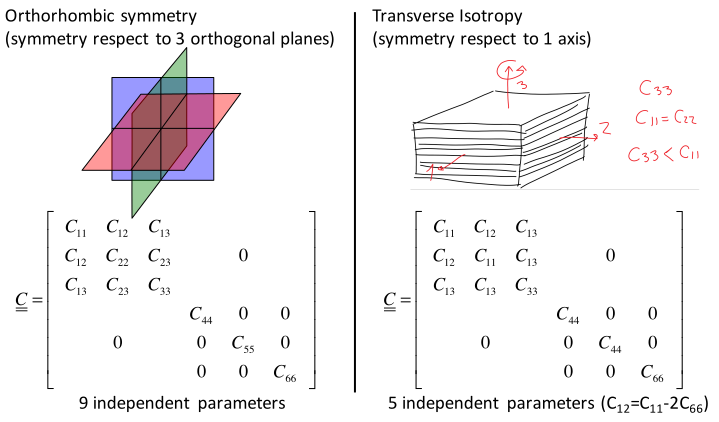
\includegraphics[scale=0.55]{.././Figures/split/4-22.pdf}%
\lthtmlpictureZ
\lthtmlcheckvsize\clearpage}

{\newpage\clearpage
\lthtmlinlinemathA{tex2html_wrap_inline21173}%
$ E_h > E_v$%
\lthtmlindisplaymathZ
\lthtmlcheckvsize\clearpage}

\stepcounter{section}
{\newpage\clearpage
\lthtmlinlinemathA{tex2html_wrap_inline21180}%
$ \varepsilon \gtrsim 0.001$%
\lthtmlindisplaymathZ
\lthtmlcheckvsize\clearpage}

{\newpage\clearpage
\lthtmlinlinemathA{tex2html_wrap_inline21182}%
$ E_{load}$%
\lthtmlindisplaymathZ
\lthtmlcheckvsize\clearpage}

{\newpage\clearpage
\lthtmlinlinemathA{tex2html_wrap_inline21184}%
$ E_{unload}$%
\lthtmlindisplaymathZ
\lthtmlcheckvsize\clearpage}

{\newpage\clearpage
\lthtmlinlinemathA{tex2html_wrap_inline21190}%
$ E_{unload} \sim E_{unload}$%
\lthtmlindisplaymathZ
\lthtmlcheckvsize\clearpage}

{\newpage\clearpage
\lthtmlpictureA{tex2html_wrap21192}%
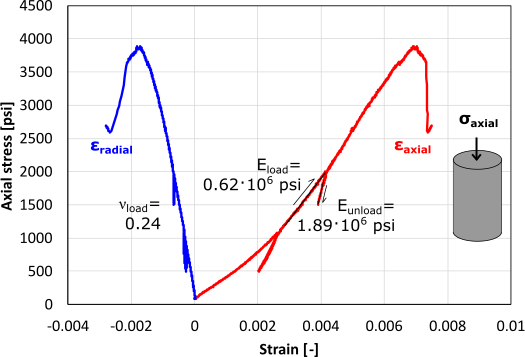
\includegraphics[scale=0.55]{.././Figures/split/LoadingUnloading.pdf}%
\lthtmlpictureZ
\lthtmlcheckvsize\clearpage}

\stepcounter{section}
{\newpage\clearpage
\lthtmlpictureA{tex2html_wrap21202}%
\includegraphics[scale=0.50]{.././Figures/split/5B-18.pdf}%
\lthtmlpictureZ
\lthtmlcheckvsize\clearpage}

{\newpage\clearpage
\lthtmlpictureA{tex2html_wrap21207}%
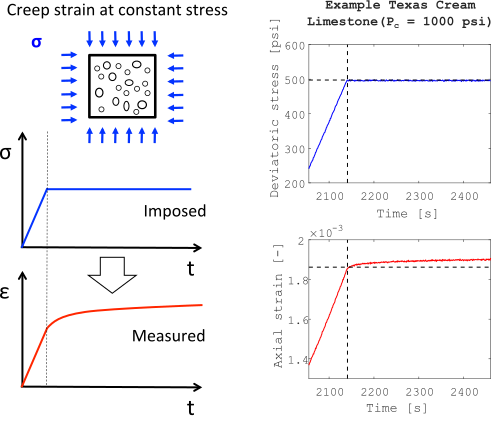
\includegraphics[scale=0.60]{.././Figures/split/5-CreepTXC.pdf}%
\lthtmlpictureZ
\lthtmlcheckvsize\clearpage}

{\newpage\clearpage
\lthtmlpictureA{tex2html_wrap21212}%
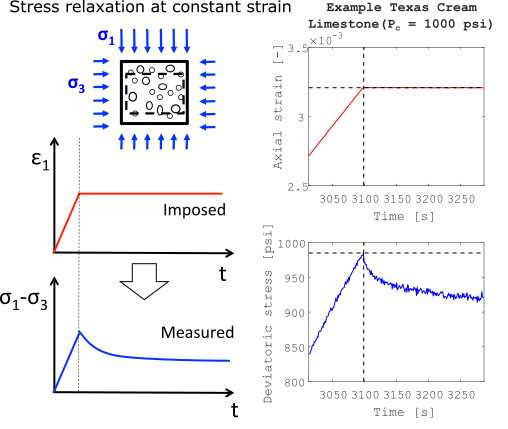
\includegraphics[scale=0.60]{.././Figures/split/5-StressRelaxTXC.pdf}%
\lthtmlpictureZ
\lthtmlcheckvsize\clearpage}

\stepcounter{section}
\stepcounter{subsection}
{\newpage\clearpage
\lthtmlinlinemathA{tex2html_wrap_inline21219}%
$ \uuline{\varepsilon} = \uuline{D} \: \uuline{\sigma}$%
\lthtmlindisplaymathZ
\lthtmlcheckvsize\clearpage}

{\newpage\clearpage
\lthtmlinlinemathA{tex2html_wrap_indisplay21221}%
$\displaystyle \uuline{\sigma} = \uuline{S} - \alpha P_p \uuline{I}$%
\lthtmlindisplaymathZ
\lthtmlcheckvsize\clearpage}

{\newpage\clearpage
\lthtmlinlinemathA{tex2html_wrap_inline21225}%
$ \uuline{I}$%
\lthtmlindisplaymathZ
\lthtmlcheckvsize\clearpage}

{\newpage\clearpage
\lthtmlinlinemathA{tex2html_wrap_indisplay21227}%
$\displaystyle \alpha = 1 - \frac{K_{drained}}{K_{unj}}$%
\lthtmlindisplaymathZ
\lthtmlcheckvsize\clearpage}

{\newpage\clearpage
\lthtmlinlinemathA{tex2html_wrap_inline21229}%
$ K_{drained}$%
\lthtmlindisplaymathZ
\lthtmlcheckvsize\clearpage}

{\newpage\clearpage
\lthtmlinlinemathA{tex2html_wrap_inline21231}%
$ K_{unj}$%
\lthtmlindisplaymathZ
\lthtmlcheckvsize\clearpage}

{\newpage\clearpage
\lthtmlinlinemathA{tex2html_wrap_inline21233}%
$ K_{unj} = K_{m}$%
\lthtmlindisplaymathZ
\lthtmlcheckvsize\clearpage}

{\newpage\clearpage
\lthtmlinlinemathA{tex2html_wrap_inline21235}%
$ \uuline{\alpha}$%
\lthtmlindisplaymathZ
\lthtmlcheckvsize\clearpage}

{\newpage\clearpage
\lthtmlinlinemathA{tex2html_wrap_inline21237}%
$ \alpha \neq 1$%
\lthtmlindisplaymathZ
\lthtmlcheckvsize\clearpage}

\stepcounter{subsection}
{\newpage\clearpage
\lthtmlpictureA{tex2html_wrap21240}%
\includegraphics[scale=0.55]{.././Figures/split/4-23.pdf}%
\lthtmlpictureZ
\lthtmlcheckvsize\clearpage}

{\newpage\clearpage
\lthtmlinlinemathA{tex2html_wrap_inline21245}%
$ \alpha_L$%
\lthtmlindisplaymathZ
\lthtmlcheckvsize\clearpage}

{\newpage\clearpage
\lthtmlinlinemathA{tex2html_wrap_inline21249}%
$ p$%
\lthtmlindisplaymathZ
\lthtmlcheckvsize\clearpage}

{\newpage\clearpage
\lthtmlinlinemathA{tex2html_wrap_indisplay21251}%
$\displaystyle \alpha_L = \left. \cfrac{1}{L} \cfrac{ \mathrm{d} L}{ \mathrm{d} T} \right|_p$%
\lthtmlindisplaymathZ
\lthtmlcheckvsize\clearpage}

{\newpage\clearpage
\lthtmlinlinemathA{tex2html_wrap_inline21253}%
$ \Delta T$%
\lthtmlindisplaymathZ
\lthtmlcheckvsize\clearpage}

{\newpage\clearpage
\lthtmldisplayA{displaymath21255}%
\begin{displaymath}\left\lbrace
\begin{array}{rcl}
\sigma_{11} & = & (\lambda + 2 \mu) \: \varepsilon_{11} + \lambda \: \varepsilon_{22} + \lambda \: \varepsilon_{33} + 3 K \alpha_L \Delta T \\
\sigma_{22} & = & \lambda \: \varepsilon_{11} + (\lambda + 2 \mu) \: \varepsilon_{22} + \lambda \: \varepsilon_{33} + 3 K \alpha_L \Delta T \\
\sigma_{33} & = & \lambda \: \varepsilon_{11} + \lambda \: \varepsilon_{22} + (\lambda + 2 \mu) \: \varepsilon_{33} + 3 K \alpha_L \Delta T \\
\sigma_{12} & = & 2 \mu \: \varepsilon_{12}\\
\sigma_{13} & = & 2 \mu \: \varepsilon_{13}\\
\sigma_{23} & = & 2 \mu \: \varepsilon_{23}\\
\end{array}
\right.\end{displaymath}%
\lthtmldisplayZ
\lthtmlcheckvsize\clearpage}

{\newpage\clearpage
\lthtmlinlinemathA{tex2html_wrap_inline21257}%
$ \sigma_{11}=\sigma_{22}=0$%
\lthtmlindisplaymathZ
\lthtmlcheckvsize\clearpage}

{\newpage\clearpage
\lthtmlinlinemathA{tex2html_wrap_inline21259}%
$ \varepsilon_{11}=\varepsilon_{22} \neq 0$%
\lthtmlindisplaymathZ
\lthtmlcheckvsize\clearpage}

{\newpage\clearpage
\lthtmlinlinemathA{tex2html_wrap_inline21261}%
$ \varepsilon_{33}=0$%
\lthtmlindisplaymathZ
\lthtmlcheckvsize\clearpage}

{\newpage\clearpage
\lthtmlinlinemathA{tex2html_wrap_inline21263}%
$ \Delta T \neq 0$%
\lthtmlindisplaymathZ
\lthtmlcheckvsize\clearpage}

{\newpage\clearpage
\lthtmldisplayA{displaymath21265}%
\begin{displaymath}\left\lbrace
\begin{array}{rcl}
0 & = & (\lambda + 2 \mu) \: \varepsilon_{11} + \lambda \: \varepsilon_{11} + 3 K \alpha_L \Delta T\\
\sigma_{33} & = & \lambda \: \varepsilon_{11} + \lambda \: \varepsilon_{11} + 3 K \alpha_L \Delta T \\
\end{array}
\right.\end{displaymath}%
\lthtmldisplayZ
\lthtmlcheckvsize\clearpage}

{\newpage\clearpage
\lthtmlinlinemathA{tex2html_wrap_indisplay21271}%
$\displaystyle \sigma_{33} = \left( \frac{6-\mu/K}{3+\mu/K} \right) K \alpha_L \Delta T \: \: \blacksquare
$%
\lthtmlindisplaymathZ
\lthtmlcheckvsize\clearpage}

\stepcounter{section}
{\newpage\clearpage
\lthtmlinlinemathA{tex2html_wrap_inline21274}%
$ D = 1.00$%
\lthtmlindisplaymathZ
\lthtmlcheckvsize\clearpage}

{\newpage\clearpage
\lthtmlinlinemathA{tex2html_wrap_inline21276}%
$ L = 2.01$%
\lthtmlindisplaymathZ
\lthtmlcheckvsize\clearpage}

{\newpage\clearpage
\lthtmlinlinemathA{tex2html_wrap_inline21278}%
$ \Delta L$%
\lthtmlindisplaymathZ
\lthtmlcheckvsize\clearpage}

{\newpage\clearpage
\lthtmlinlinemathA{tex2html_wrap_inline21280}%
$ \Delta D$%
\lthtmlindisplaymathZ
\lthtmlcheckvsize\clearpage}

{\newpage\clearpage
\lthtmlinlinemathA{tex2html_wrap_inline21283}%
$ \uline{\sigma} = \uuline{C} \: \uline{\varepsilon}$%
\lthtmlindisplaymathZ
\lthtmlcheckvsize\clearpage}

{\newpage\clearpage
\lthtmlinlinemathA{tex2html_wrap_inline21285}%
$ \sigma_{iso}$%
\lthtmlindisplaymathZ
\lthtmlcheckvsize\clearpage}

{\newpage\clearpage
\lthtmlinlinemathA{tex2html_wrap_inline21287}%
$ \varepsilon_{vol}=\frac{3(1-2\nu)}{E} \sigma_{iso}$%
\lthtmlindisplaymathZ
\lthtmlcheckvsize\clearpage}

{\newpage\clearpage
\lthtmlinlinemathA{tex2html_wrap_inline21289}%
$ \varepsilon_{vol}$%
\lthtmlindisplaymathZ
\lthtmlcheckvsize\clearpage}

{\newpage\clearpage
\lthtmlinlinemathA{tex2html_wrap_inline21291}%
$ E = 4$%
\lthtmlindisplaymathZ
\lthtmlcheckvsize\clearpage}

{\newpage\clearpage
\lthtmlinlinemathA{tex2html_wrap_inline21293}%
$ \nu = 0.2$%
\lthtmlindisplaymathZ
\lthtmlcheckvsize\clearpage}

{\newpage\clearpage
\lthtmlinlinemathA{tex2html_wrap_inline21295}%
$ \sigma_{iso} =$%
\lthtmlindisplaymathZ
\lthtmlcheckvsize\clearpage}

{\newpage\clearpage
\lthtmlinlinemathA{tex2html_wrap_inline21297}%
$ \times$%
\lthtmlindisplaymathZ
\lthtmlcheckvsize\clearpage}

{\newpage\clearpage
\lthtmlinlinemathA{tex2html_wrap_inline21303}%
$ \sigma_{11} = \cfrac{E(1-\nu)}{(1+\nu)(1-2\nu)} \varepsilon_{11}$%
\lthtmlindisplaymathZ
\lthtmlcheckvsize\clearpage}

{\newpage\clearpage
\lthtmlinlinemathA{tex2html_wrap_inline21307}%
$ 3 \times 3$%
\lthtmlindisplaymathZ
\lthtmlcheckvsize\clearpage}

{\newpage\clearpage
\lthtmlinlinemathA{tex2html_wrap_inline21309}%
$ \phi = 0.35$%
\lthtmlindisplaymathZ
\lthtmlcheckvsize\clearpage}

\stepcounter{section}
\stepcounter{chapter}
\stepcounter{section}
\stepcounter{subsection}
{\newpage\clearpage
\lthtmlpictureA{tex2html_wrap21327}%
\includegraphics[scale=0.65]{.././Figures/split/5A-3.pdf}%
\lthtmlpictureZ
\lthtmlcheckvsize\clearpage}

\stepcounter{subsection}
{\newpage\clearpage
\lthtmlpictureA{tex2html_wrap21333}%
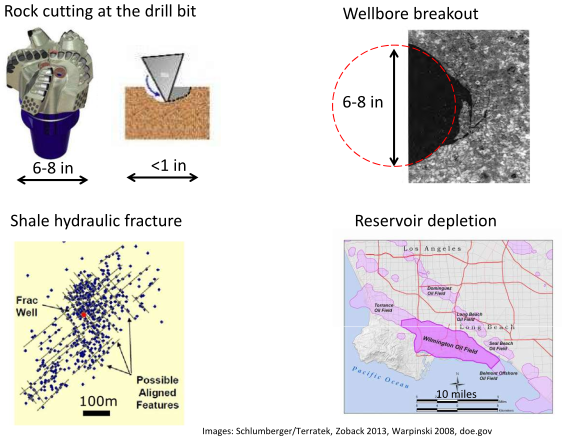
\includegraphics[scale=0.65]{.././Figures/split/5A-4.pdf}%
\lthtmlpictureZ
\lthtmlcheckvsize\clearpage}

\stepcounter{subsection}
{\newpage\clearpage
\lthtmlpictureA{tex2html_wrap21339}%
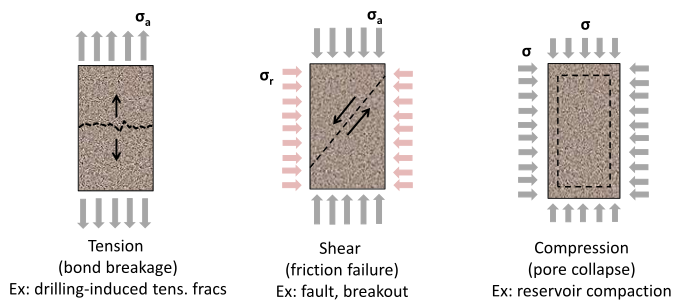
\includegraphics[scale=0.55]{.././Figures/split/5A-5.pdf}%
\lthtmlpictureZ
\lthtmlcheckvsize\clearpage}

\stepcounter{section}
\stepcounter{subsection}
{\newpage\clearpage
\lthtmlpictureA{tex2html_wrap21346}%
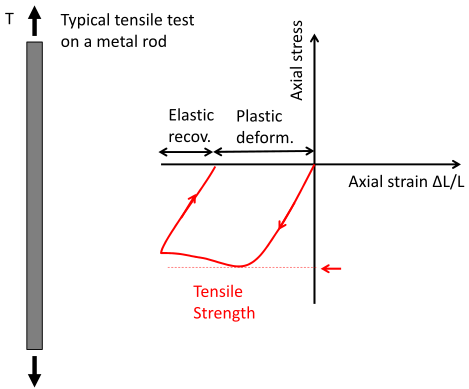
\includegraphics[scale=0.55]{.././Figures/split/5A-6.pdf}%
\lthtmlpictureZ
\lthtmlcheckvsize\clearpage}

{\newpage\clearpage
\lthtmlpictureA{tex2html_wrap21351}%
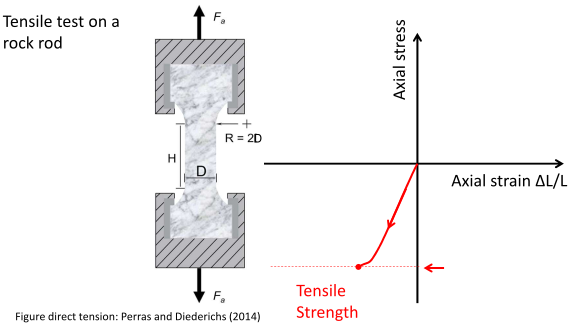
\includegraphics[scale=0.60]{.././Figures/split/5A-7.pdf}%
\lthtmlpictureZ
\lthtmlcheckvsize\clearpage}

\stepcounter{subsection}
{\newpage\clearpage
\lthtmlinlinemathA{tex2html_wrap_indisplay21359}%
$\displaystyle T_S = \frac{P_B}{\pi L R}$%
\lthtmlindisplaymathZ
\lthtmlcheckvsize\clearpage}

{\newpage\clearpage
\lthtmlinlinemathA{tex2html_wrap_inline21361}%
$ P_B$%
\lthtmlindisplaymathZ
\lthtmlcheckvsize\clearpage}

{\newpage\clearpage
\lthtmlinlinemathA{tex2html_wrap_inline21365}%
$ R$%
\lthtmlindisplaymathZ
\lthtmlcheckvsize\clearpage}

{\newpage\clearpage
\lthtmlpictureA{tex2html_wrap21367}%
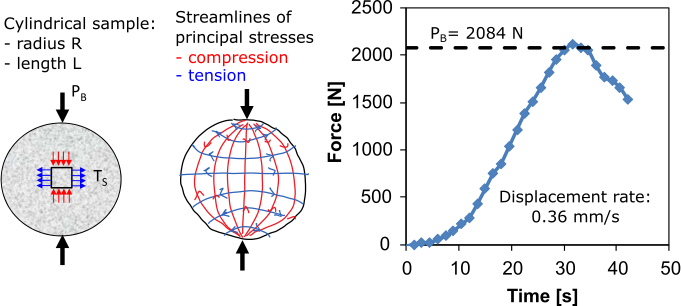
\includegraphics[scale=0.55]{.././Figures/split/4-TensileStrength.pdf}%
\lthtmlpictureZ
\lthtmlcheckvsize\clearpage}

{\newpage\clearpage
\lthtmlinlinemathA{tex2html_wrap_indisplay21372}%
$\displaystyle R = \frac{1}{2}$%
\lthtmlindisplaymathZ
\lthtmlcheckvsize\clearpage}

{\newpage\clearpage
\lthtmlinlinemathA{tex2html_wrap_indisplay21373}%
$\displaystyle = 0.0127$%
\lthtmlindisplaymathZ
\lthtmlcheckvsize\clearpage}

{\newpage\clearpage
\lthtmlinlinemathA{tex2html_wrap_indisplay21375}%
$\displaystyle L = 1$%
\lthtmlindisplaymathZ
\lthtmlcheckvsize\clearpage}

{\newpage\clearpage
\lthtmlinlinemathA{tex2html_wrap_indisplay21376}%
$\displaystyle = 0.0254$%
\lthtmlindisplaymathZ
\lthtmlcheckvsize\clearpage}

{\newpage\clearpage
\lthtmlinlinemathA{tex2html_wrap_indisplay21378}%
$\displaystyle T_S = \frac{2084 \text { N}}{\pi (0.0254 \text{ m}) (0.0127 \text{ m})}
= 2.06 \times 10^6 \text{ Pa} = 2.06 \text{ MPa} \: \: \blacksquare$%
\lthtmlindisplaymathZ
\lthtmlcheckvsize\clearpage}

{\newpage\clearpage
\lthtmlpictureA{tex2html_wrap21380}%
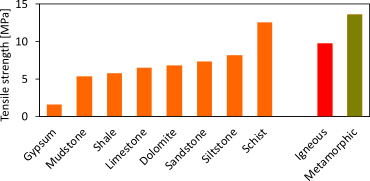
\includegraphics[scale=0.65]{.././Figures/split/4-TensStrengthSummary.pdf}%
\lthtmlpictureZ
\lthtmlcheckvsize\clearpage}

\stepcounter{section}
\stepcounter{subsection}
{\newpage\clearpage
\lthtmlinlinemathA{tex2html_wrap_inline21387}%
$ S_0$%
\lthtmlindisplaymathZ
\lthtmlcheckvsize\clearpage}

{\newpage\clearpage
\lthtmlinlinemathA{tex2html_wrap_inline21389}%
$ F_T$%
\lthtmlindisplaymathZ
\lthtmlcheckvsize\clearpage}

{\newpage\clearpage
\lthtmlinlinemathA{tex2html_wrap_inline21393}%
$ F_N$%
\lthtmlindisplaymathZ
\lthtmlcheckvsize\clearpage}

{\newpage\clearpage
\lthtmlinlinemathA{tex2html_wrap_inline21395}%
$ F_T = \mu F_N$%
\lthtmlindisplaymathZ
\lthtmlcheckvsize\clearpage}

{\newpage\clearpage
\lthtmlinlinemathA{tex2html_wrap_inline21397}%
$ F_N=0$%
\lthtmlindisplaymathZ
\lthtmlcheckvsize\clearpage}

{\newpage\clearpage
\lthtmlinlinemathA{tex2html_wrap_inline21399}%
$ F_T = 0$%
\lthtmlindisplaymathZ
\lthtmlcheckvsize\clearpage}

{\newpage\clearpage
\lthtmlpictureA{tex2html_wrap21405}%
\includegraphics[scale=0.45]{.././Figures/split/5A-10.pdf}%
\lthtmlpictureZ
\lthtmlcheckvsize\clearpage}

{\newpage\clearpage
\lthtmlinlinemathA{tex2html_wrap_inline21410}%
$ \tau$%
\lthtmlindisplaymathZ
\lthtmlcheckvsize\clearpage}

{\newpage\clearpage
\lthtmlinlinemathA{tex2html_wrap_inline21412}%
$ \sigma_n$%
\lthtmlindisplaymathZ
\lthtmlcheckvsize\clearpage}

{\newpage\clearpage
\lthtmlinlinemathA{tex2html_wrap_inline21414}%
$ \mu_i$%
\lthtmlindisplaymathZ
\lthtmlcheckvsize\clearpage}

{\newpage\clearpage
\lthtmlinlinemathA{tex2html_wrap_inline21416}%
$ \tau = \mu_i \sigma_n$%
\lthtmlindisplaymathZ
\lthtmlcheckvsize\clearpage}

{\newpage\clearpage
\lthtmlpictureA{tex2html_wrap21418}%
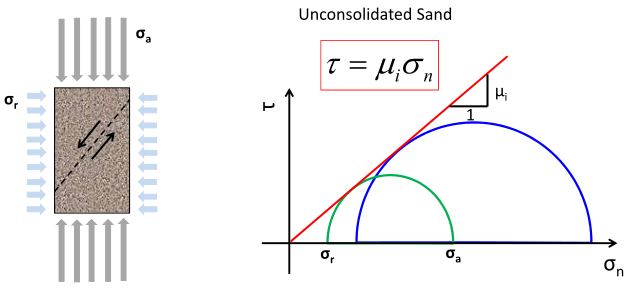
\includegraphics[scale=0.50]{.././Figures/split/5A-14.pdf}%
\lthtmlpictureZ
\lthtmlcheckvsize\clearpage}

{\newpage\clearpage
\lthtmlinlinemathA{tex2html_wrap_inline21429}%
$ \sigma_n = 0$%
\lthtmlindisplaymathZ
\lthtmlcheckvsize\clearpage}

{\newpage\clearpage
\lthtmlinlinemathA{tex2html_wrap_inline21431}%
$ \tau = 0$%
\lthtmlindisplaymathZ
\lthtmlcheckvsize\clearpage}

{\newpage\clearpage
\lthtmlinlinemathA{tex2html_wrap_inline21435}%
$ \varphi$%
\lthtmlindisplaymathZ
\lthtmlcheckvsize\clearpage}

{\newpage\clearpage
\lthtmlinlinemathA{tex2html_wrap_inline21437}%
$ \tan (\varphi) = \mu_i$%
\lthtmlindisplaymathZ
\lthtmlcheckvsize\clearpage}

{\newpage\clearpage
\lthtmlinlinemathA{tex2html_wrap_inline21441}%
$ \mu_i=0.5$%
\lthtmlindisplaymathZ
\lthtmlcheckvsize\clearpage}

{\newpage\clearpage
\lthtmlinlinemathA{tex2html_wrap_inline21443}%
$ \varphi \sim 30^{\circ}$%
\lthtmlindisplaymathZ
\lthtmlcheckvsize\clearpage}

\stepcounter{subsection}
{\newpage\clearpage
\lthtmlinlinemathA{tex2html_wrap_inline21446}%
$ \sigma_r = 0$%
\lthtmlindisplaymathZ
\lthtmlcheckvsize\clearpage}

{\newpage\clearpage
\lthtmlpictureA{tex2html_wrap21454}%
\includegraphics[scale=0.60]{.././Figures/split/5A-12.pdf}%
\lthtmlpictureZ
\lthtmlcheckvsize\clearpage}

\stepcounter{subsection}
{\newpage\clearpage
\lthtmlinlinemathA{tex2html_wrap_inline21460}%
$ \sigma_r \neq 0$%
\lthtmlindisplaymathZ
\lthtmlcheckvsize\clearpage}

{\newpage\clearpage
\lthtmlinlinemathA{tex2html_wrap_indisplay21468}%
$\displaystyle \tau = S_0 + \mu_i \sigma_n$%
\lthtmlindisplaymathZ
\lthtmlcheckvsize\clearpage}

{\newpage\clearpage
\lthtmlpictureA{tex2html_wrap21470}%
\includegraphics[scale=0.60]{.././Figures/split/5A-13.pdf}%
\lthtmlpictureZ
\lthtmlcheckvsize\clearpage}

{\newpage\clearpage
\lthtmlinlinemathA{tex2html_wrap_inline21479}%
$ \pi/4 + \varphi/2$%
\lthtmlindisplaymathZ
\lthtmlcheckvsize\clearpage}

{\newpage\clearpage
\lthtmlinlinemathA{tex2html_wrap_inline21483}%
$ \pi/4 + \varphi/2 = 60^{\circ}$%
\lthtmlindisplaymathZ
\lthtmlcheckvsize\clearpage}

{\newpage\clearpage
\lthtmlinlinemathA{tex2html_wrap_inline21487}%
$ \sigma_a / \sigma_r$%
\lthtmlindisplaymathZ
\lthtmlcheckvsize\clearpage}

{\newpage\clearpage
\lthtmlpictureA{tex2html_wrap21489}%
\includegraphics[scale=0.50]{.././Figures/split/5A-15.pdf}%
\lthtmlpictureZ
\lthtmlcheckvsize\clearpage}

{\newpage\clearpage
\lthtmlinlinemathA{tex2html_wrap_inline21493}%
$ \tau / \sigma_n = \mu_i$%
\lthtmlindisplaymathZ
\lthtmlcheckvsize\clearpage}

{\newpage\clearpage
\lthtmlpictureA{tex2html_wrap21495}%
\includegraphics[scale=0.55]{.././Figures/split/AngleFailurePlane.pdf}%
\lthtmlpictureZ
\lthtmlcheckvsize\clearpage}

{\newpage\clearpage
\lthtmlinlinemathA{tex2html_wrap_inline21497}%
$ (\sigma_a,0)$%
\lthtmlindisplaymathZ
\lthtmlcheckvsize\clearpage}

{\newpage\clearpage
\lthtmlinlinemathA{tex2html_wrap_inline21503}%
$ (\sigma_r,0)$%
\lthtmlindisplaymathZ
\lthtmlcheckvsize\clearpage}

{\newpage\clearpage
\lthtmlinlinemathA{tex2html_wrap_inline21509}%
$ (\sigma_n,\tau)$%
\lthtmlindisplaymathZ
\lthtmlcheckvsize\clearpage}

{\newpage\clearpage
\lthtmlinlinemathA{tex2html_wrap_inline21511}%
$ \pi/2 + \varphi$%
\lthtmlindisplaymathZ
\lthtmlcheckvsize\clearpage}

{\newpage\clearpage
\lthtmlinlinemathA{tex2html_wrap_inline21517}%
$ (\pi/2 + \varphi)/2$%
\lthtmlindisplaymathZ
\lthtmlcheckvsize\clearpage}

{\newpage\clearpage
\lthtmlinlinemathA{tex2html_wrap_inline21523}%
$ ^{\circ} = \pi/2$%
\lthtmlindisplaymathZ
\lthtmlcheckvsize\clearpage}

{\newpage\clearpage
\lthtmlinlinemathA{tex2html_wrap_inline21525}%
$ C$%
\lthtmlindisplaymathZ
\lthtmlcheckvsize\clearpage}

{\newpage\clearpage
\lthtmlinlinemathA{tex2html_wrap_indisplay21531}%
$\displaystyle \frac{\sigma_a}{\sigma_r} = \frac{C + R}{C-R} = 
		\frac{C+C \sin \varphi}{C-C \sin \varphi} =
		\frac{1+\sin \varphi}{1-\sin \varphi} =		
 \: \: \blacksquare
$%
\lthtmlindisplaymathZ
\lthtmlcheckvsize\clearpage}

{\newpage\clearpage
\lthtmlinlinemathA{tex2html_wrap_indisplay21533}%
$\displaystyle \sigma_1 = UCS + q \: \sigma_3$%
\lthtmlindisplaymathZ
\lthtmlcheckvsize\clearpage}

{\newpage\clearpage
\lthtmlinlinemathA{tex2html_wrap_inline21539}%
$ q$%
\lthtmlindisplaymathZ
\lthtmlcheckvsize\clearpage}

{\newpage\clearpage
\lthtmlinlinemathA{tex2html_wrap_inline21543}%
$ p'-q$%
\lthtmlindisplaymathZ
\lthtmlcheckvsize\clearpage}

{\newpage\clearpage
\lthtmlinlinemathA{tex2html_wrap_inline21545}%
$ \sigma_m-q$%
\lthtmlindisplaymathZ
\lthtmlcheckvsize\clearpage}

{\newpage\clearpage
\lthtmlinlinemathA{tex2html_wrap_indisplay21547}%
$\displaystyle q = \frac{1 + \sin \varphi}{1 - \sin \varphi}$%
\lthtmlindisplaymathZ
\lthtmlcheckvsize\clearpage}

{\newpage\clearpage
\lthtmlinlinemathA{tex2html_wrap_inline21549}%
$ \varphi ~ 30^{\circ}$%
\lthtmlindisplaymathZ
\lthtmlcheckvsize\clearpage}

{\newpage\clearpage
\lthtmlinlinemathA{tex2html_wrap_inline21551}%
$ q = 3$%
\lthtmlindisplaymathZ
\lthtmlcheckvsize\clearpage}

{\newpage\clearpage
\lthtmlinlinemathA{tex2html_wrap_indisplay21555}%
$\displaystyle UCS = 2 S_0 \left( \frac{1 + \sin \varphi}{1 - \sin \varphi} \right)^{1/2}
= 2 S_0 \sqrt{q}$%
\lthtmlindisplaymathZ
\lthtmlcheckvsize\clearpage}

{\newpage\clearpage
\lthtmlpictureA{tex2html_wrap21557}%
\includegraphics[scale=0.65]{.././Figures/split/5A-16.pdf}%
\lthtmlpictureZ
\lthtmlcheckvsize\clearpage}

{\newpage\clearpage
\lthtmlpictureA{tex2html_wrap21562}%
\includegraphics[scale=0.85]{.././Figures/split/4-ShearStrengthSummary.pdf}%
\lthtmlpictureZ
\lthtmlcheckvsize\clearpage}

\stepcounter{subsection}
{\newpage\clearpage
\lthtmlinlinemathA{tex2html_wrap_inline21568}%
$ (S_1,S_2,S_3)$%
\lthtmlindisplaymathZ
\lthtmlcheckvsize\clearpage}

{\newpage\clearpage
\lthtmlinlinemathA{tex2html_wrap_inline21570}%
$ (\sigma_1,\sigma_2,\sigma_3)$%
\lthtmlindisplaymathZ
\lthtmlcheckvsize\clearpage}

{\newpage\clearpage
\lthtmlinlinemathA{tex2html_wrap_inline21572}%
$ P_c$%
\lthtmlindisplaymathZ
\lthtmlcheckvsize\clearpage}

{\newpage\clearpage
\lthtmlinlinemathA{tex2html_wrap_inline21574}%
$ \sigma_D$%
\lthtmlindisplaymathZ
\lthtmlcheckvsize\clearpage}

{\newpage\clearpage
\lthtmlinlinemathA{tex2html_wrap_inline21580}%
$ P_c = cst$%
\lthtmlindisplaymathZ
\lthtmlcheckvsize\clearpage}

{\newpage\clearpage
\lthtmlinlinemathA{tex2html_wrap_inline21584}%
$ P_p < P_c$%
\lthtmlindisplaymathZ
\lthtmlcheckvsize\clearpage}

{\newpage\clearpage
\lthtmlinlinemathA{tex2html_wrap_inline21586}%
$ P_p = cst$%
\lthtmlindisplaymathZ
\lthtmlcheckvsize\clearpage}

{\newpage\clearpage
\lthtmlinlinemathA{tex2html_wrap_inline21590}%
$ \sigma_D =S_1 - S_3$%
\lthtmlindisplaymathZ
\lthtmlcheckvsize\clearpage}

{\newpage\clearpage
\lthtmlinlinemathA{tex2html_wrap_inline21596}%
$ S_3 = P_c$%
\lthtmlindisplaymathZ
\lthtmlcheckvsize\clearpage}

{\newpage\clearpage
\lthtmlinlinemathA{tex2html_wrap_inline21598}%
$ S_2=S_3$%
\lthtmlindisplaymathZ
\lthtmlcheckvsize\clearpage}

{\newpage\clearpage
\lthtmlinlinemathA{tex2html_wrap_inline21600}%
$ S_1 - S_3=\sigma_1-\sigma_3$%
\lthtmlindisplaymathZ
\lthtmlcheckvsize\clearpage}

{\newpage\clearpage
\lthtmlinlinemathA{tex2html_wrap_inline21602}%
$ d \varepsilon_a / dt = cst$%
\lthtmlindisplaymathZ
\lthtmlcheckvsize\clearpage}

{\newpage\clearpage
\lthtmlinlinemathA{tex2html_wrap_inline21616}%
$ \sigma_1 = (S_1 - P_p)$%
\lthtmlindisplaymathZ
\lthtmlcheckvsize\clearpage}

{\newpage\clearpage
\lthtmlinlinemathA{tex2html_wrap_inline21618}%
$ \sigma_3 = (S_3 - P_p)$%
\lthtmlindisplaymathZ
\lthtmlcheckvsize\clearpage}

{\newpage\clearpage
\lthtmlinlinemathA{tex2html_wrap_indisplay21628}%
$\displaystyle \varphi = \arctan \left( \frac{q-1}{2\sqrt{q}} \right)$%
\lthtmlindisplaymathZ
\lthtmlcheckvsize\clearpage}

{\newpage\clearpage
\lthtmlinlinemathA{tex2html_wrap_inline21640}%
$ S_3 \leqslant 80$%
\lthtmlindisplaymathZ
\lthtmlcheckvsize\clearpage}

{\newpage\clearpage
\lthtmlinlinemathA{tex2html_wrap_inline21642}%
$ S_1 \sim 80$%
\lthtmlindisplaymathZ
\lthtmlcheckvsize\clearpage}

{\newpage\clearpage
\lthtmlinlinemathA{tex2html_wrap_indisplay21644}%
$\displaystyle UCS = 80$%
\lthtmlindisplaymathZ
\lthtmlcheckvsize\clearpage}

{\newpage\clearpage
\lthtmlinlinemathA{tex2html_wrap_indisplay21645}%
$\displaystyle $%
\lthtmlindisplaymathZ
\lthtmlcheckvsize\clearpage}

{\newpage\clearpage
\lthtmlinlinemathA{tex2html_wrap_indisplay21649}%
$\displaystyle q = \frac{\Delta \sigma_1}{\Delta \sigma_3} = 
       \frac{520 \text{ MPa}}{110 \text{ MPa}} = 4.73
$%
\lthtmlindisplaymathZ
\lthtmlcheckvsize\clearpage}

{\newpage\clearpage
\lthtmlinlinemathA{tex2html_wrap_indisplay21651}%
$\displaystyle S_0 = \frac{UCS}{2 \sqrt{q}} = \frac{80 \text{MPa}}{2 \sqrt{4.73}} = 18.4 \text{MPa} $%
\lthtmlindisplaymathZ
\lthtmlcheckvsize\clearpage}

{\newpage\clearpage
\lthtmlinlinemathA{tex2html_wrap_indisplay21653}%
$\displaystyle \varphi = \arctan \left( \frac{q-1}{2\sqrt{q}} \right) 
        = \arctan \left( \frac{4.73-1}{2\sqrt{4.73}} \right) = 40.6^{\circ} 
$%
\lthtmlindisplaymathZ
\lthtmlcheckvsize\clearpage}

{\newpage\clearpage
\lthtmlinlinemathA{tex2html_wrap_indisplay21655}%
$\displaystyle \mu_i = \tan (\varphi) = \tan (40.6^{\circ}) = 0.86 
\: \: \blacksquare
$%
\lthtmlindisplaymathZ
\lthtmlcheckvsize\clearpage}

{\newpage\clearpage
\lthtmlinlinemathA{tex2html_wrap_inline21657}%
$ \varepsilon_v = \varepsilon_a + 2\varepsilon_r$%
\lthtmlindisplaymathZ
\lthtmlcheckvsize\clearpage}

{\newpage\clearpage
\lthtmlinlinemathA{tex2html_wrap_inline21659}%
$ d \varepsilon_v/dt<0$%
\lthtmlindisplaymathZ
\lthtmlcheckvsize\clearpage}

{\newpage\clearpage
\lthtmlpictureA{tex2html_wrap21661}%
\includegraphics[scale=0.65]{.././Figures/split/Triaxial-Darley.pdf}%
\lthtmlpictureZ
\lthtmlcheckvsize\clearpage}

\stepcounter{section}
{\newpage\clearpage
\lthtmlpictureA{tex2html_wrap21669}%
\includegraphics[scale=0.65]{.././Figures/split/5A-21.pdf}%
\lthtmlpictureZ
\lthtmlcheckvsize\clearpage}

\stepcounter{section}
{\newpage\clearpage
\lthtmlinlinemathA{tex2html_wrap_inline21683}%
$ \tau = S_0 + \mu_i \sigma_n$%
\lthtmlindisplaymathZ
\lthtmlcheckvsize\clearpage}

{\newpage\clearpage
\lthtmlpictureA{tex2html_wrap21685}%
\includegraphics[scale=0.55]{.././Figures/split/5B-YieldLocus.pdf}%
\lthtmlpictureZ
\lthtmlcheckvsize\clearpage}

\stepcounter{section}
{\newpage\clearpage
\lthtmlinlinemathA{tex2html_wrap_inline21691}%
$ \beta_w$%
\lthtmlindisplaymathZ
\lthtmlcheckvsize\clearpage}

{\newpage\clearpage
\lthtmlinlinemathA{tex2html_wrap_inline21695}%
$ S_w + \mu_w \sigma_n$%
\lthtmlindisplaymathZ
\lthtmlcheckvsize\clearpage}

{\newpage\clearpage
\lthtmlpictureA{tex2html_wrap21697}%
\includegraphics[scale=0.75]{.././Figures/split/5B-8.pdf}%
\lthtmlpictureZ
\lthtmlcheckvsize\clearpage}

\stepcounter{section}
{\newpage\clearpage
\lthtmlpictureA{tex2html_wrap21703}%
\includegraphics[scale=0.65]{.././Figures/split/5B-9.pdf}%
\lthtmlpictureZ
\lthtmlcheckvsize\clearpage}

{\newpage\clearpage
\lthtmlpictureA{tex2html_wrap21708}%
\includegraphics[scale=0.65]{.././Figures/split/5B-10.pdf}%
\lthtmlpictureZ
\lthtmlcheckvsize\clearpage}

{\newpage\clearpage
\lthtmlinlinemathA{tex2html_wrap_inline21713}%
$ \sigma_d = (\sigma_1 - \sigma_3)$%
\lthtmlindisplaymathZ
\lthtmlcheckvsize\clearpage}

{\newpage\clearpage
\lthtmlinlinemathA{tex2html_wrap_inline21715}%
$ \uuline{\varepsilon}{}_p$%
\lthtmlindisplaymathZ
\lthtmlcheckvsize\clearpage}

{\newpage\clearpage
\lthtmlinlinemathA{tex2html_wrap_inline21717}%
$ \uuline{C}{}_p$%
\lthtmlindisplaymathZ
\lthtmlcheckvsize\clearpage}

{\newpage\clearpage
\lthtmlinlinemathA{tex2html_wrap_indisplay21719}%
$\displaystyle \Delta \uuline{\sigma} = \uuline{C}{}_p \Delta \uuline{\varepsilon}{}_p$%
\lthtmlindisplaymathZ
\lthtmlcheckvsize\clearpage}

{\newpage\clearpage
\lthtmlpictureA{tex2html_wrap21721}%
\includegraphics[scale=0.60]{.././Figures/split/5B-11.pdf}%
\lthtmlpictureZ
\lthtmlcheckvsize\clearpage}

\stepcounter{section}
{\newpage\clearpage
\lthtmlpictureA{tex2html_wrap21727}%
\includegraphics[scale=0.65]{.././Figures/split/5B-12.pdf}%
\lthtmlpictureZ
\lthtmlcheckvsize\clearpage}

{\newpage\clearpage
\lthtmlpictureA{tex2html_wrap21732}%
\includegraphics[scale=0.60]{.././Figures/split/5B-13.pdf}%
\lthtmlpictureZ
\lthtmlcheckvsize\clearpage}

{\newpage\clearpage
\lthtmlpictureA{tex2html_wrap21737}%
\includegraphics[scale=0.55]{.././Figures/split/5B-14.pdf}%
\lthtmlpictureZ
\lthtmlcheckvsize\clearpage}

\stepcounter{section}
{\newpage\clearpage
\lthtmlinlinemathA{tex2html_wrap_inline21747}%
$ S_1 - S_3$%
\lthtmlindisplaymathZ
\lthtmlcheckvsize\clearpage}

{\newpage\clearpage
\lthtmlinlinemathA{tex2html_wrap_inline21773}%
$ \varphi = f(q)$%
\lthtmlindisplaymathZ
\lthtmlcheckvsize\clearpage}

{\newpage\clearpage
\lthtmlinlinemathA{tex2html_wrap_inline21779}%
$ Sig_D$%
\lthtmlindisplaymathZ
\lthtmlcheckvsize\clearpage}

{\newpage\clearpage
\lthtmlinlinemathA{tex2html_wrap_inline21783}%
$ E_x$%
\lthtmlindisplaymathZ
\lthtmlcheckvsize\clearpage}

{\newpage\clearpage
\lthtmlinlinemathA{tex2html_wrap_inline21785}%
$ E_y$%
\lthtmlindisplaymathZ
\lthtmlcheckvsize\clearpage}

{\newpage\clearpage
\lthtmlinlinemathA{tex2html_wrap_inline21787}%
$ q=5.3$%
\lthtmlindisplaymathZ
\lthtmlcheckvsize\clearpage}

{\newpage\clearpage
\lthtmlinlinemathA{tex2html_wrap_inline21793}%
$ S_1=S_3 \rightarrow S_1-S_3=0$%
\lthtmlindisplaymathZ
\lthtmlcheckvsize\clearpage}

{\newpage\clearpage
\lthtmlinlinemathA{tex2html_wrap_inline21854}%
$ S_o$%
\lthtmlindisplaymathZ
\lthtmlcheckvsize\clearpage}

\stepcounter{section}
\stepcounter{chapter}
\stepcounter{section}
{\newpage\clearpage
\lthtmlpictureA{tex2html_wrap21865}%
\includegraphics[scale=0.60]{.././Figures/split/6-2.pdf}%
\lthtmlpictureZ
\lthtmlcheckvsize\clearpage}

\stepcounter{section}
{\newpage\clearpage
\lthtmlpictureA{tex2html_wrap21871}%
\includegraphics[scale=0.60]{.././Figures/split/6-8.pdf}%
\lthtmlpictureZ
\lthtmlcheckvsize\clearpage}

\stepcounter{subsection}
{\newpage\clearpage
\lthtmlinlinemathA{tex2html_wrap_inline21881}%
$ dip$%
\lthtmlindisplaymathZ
\lthtmlcheckvsize\clearpage}

{\newpage\clearpage
\lthtmlpictureA{tex2html_wrap21907}%
\includegraphics[scale=0.65]{.././Figures/split/6-5.pdf}%
\lthtmlpictureZ
\lthtmlcheckvsize\clearpage}

\stepcounter{subsection}
\stepcounter{subsection}
{\newpage\clearpage
\lthtmlpictureA{tex2html_wrap21940}%
\includegraphics[scale=0.55]{.././Figures/split/6-7.pdf}%
\lthtmlpictureZ
\lthtmlcheckvsize\clearpage}

\stepcounter{section}
\stepcounter{subsection}
{\newpage\clearpage
\lthtmlinlinemathA{tex2html_wrap_indisplay21961}%
$\displaystyle \sigma_1 = q \: \sigma_3$%
\lthtmlindisplaymathZ
\lthtmlcheckvsize\clearpage}

{\newpage\clearpage
\lthtmlinlinemathA{tex2html_wrap_indisplay21963}%
$\displaystyle q = \left( \sqrt{\mu^2 +1} + \mu \right) ^2 = \frac{1+\sin \: \varphi}{1-\sin \: \varphi}$%
\lthtmlindisplaymathZ
\lthtmlcheckvsize\clearpage}

{\newpage\clearpage
\lthtmlinlinemathA{tex2html_wrap_inline21967}%
$ \sigma_1/\sigma_3 \sim $%
\lthtmlindisplaymathZ
\lthtmlcheckvsize\clearpage}

{\newpage\clearpage
\lthtmlpictureA{tex2html_wrap21969}%
\includegraphics[scale=0.65]{.././Figures/split/6-20.pdf}%
\lthtmlpictureZ
\lthtmlcheckvsize\clearpage}

{\newpage\clearpage
\lthtmlinlinemathA{tex2html_wrap_inline21983}%
$ \pi/4 + \phi/2$%
\lthtmlindisplaymathZ
\lthtmlcheckvsize\clearpage}

{\newpage\clearpage
\lthtmlinlinemathA{tex2html_wrap_inline21985}%
$ \sim 30 ^{\circ}$%
\lthtmlindisplaymathZ
\lthtmlcheckvsize\clearpage}

{\newpage\clearpage
\lthtmlinlinemathA{tex2html_wrap_inline21987}%
$ \sim 60 ^{\circ}$%
\lthtmlindisplaymathZ
\lthtmlcheckvsize\clearpage}

{\newpage\clearpage
\lthtmlinlinemathA{tex2html_wrap_inline21989}%
$ 45 ^{\circ}$%
\lthtmlindisplaymathZ
\lthtmlcheckvsize\clearpage}

{\newpage\clearpage
\lthtmlinlinemathA{tex2html_wrap_inline21991}%
$ 67.5 ^{\circ}$%
\lthtmlindisplaymathZ
\lthtmlcheckvsize\clearpage}

{\newpage\clearpage
\lthtmlinlinemathA{tex2html_wrap_inline21993}%
$ 50 ^{\circ}$%
\lthtmlindisplaymathZ
\lthtmlcheckvsize\clearpage}

{\newpage\clearpage
\lthtmlinlinemathA{tex2html_wrap_inline21995}%
$ 70 ^{\circ}$%
\lthtmlindisplaymathZ
\lthtmlcheckvsize\clearpage}

{\newpage\clearpage
\lthtmlinlinemathA{tex2html_wrap_inline22013}%
$ \sigma_1 / \sigma_3 > q$%
\lthtmlindisplaymathZ
\lthtmlcheckvsize\clearpage}

{\newpage\clearpage
\lthtmlinlinemathA{tex2html_wrap_inline22015}%
$ \sigma_1 / \sigma_3 < q$%
\lthtmlindisplaymathZ
\lthtmlcheckvsize\clearpage}

\stepcounter{subsection}
{\newpage\clearpage
\lthtmldisplayA{displaymath22018}%
\begin{displaymath}\left\lbrace
\begin{array}{l}
S_1 = S_v \\
S_2 = S_{Hmax} \\
S_3 = S_{hmin} \\
\end{array}
\right.\end{displaymath}%
\lthtmldisplayZ
\lthtmlcheckvsize\clearpage}

{\newpage\clearpage
\lthtmlinlinemathA{tex2html_wrap_inline22020}%
$ S_1 > S_2 > S_3$%
\lthtmlindisplaymathZ
\lthtmlcheckvsize\clearpage}

{\newpage\clearpage
\lthtmlpictureA{tex2html_wrap22032}%
\includegraphics[scale=0.50]{.././Figures/split/6-12.pdf}%
\lthtmlpictureZ
\lthtmlcheckvsize\clearpage}

{\newpage\clearpage
\lthtmlinlinemathA{tex2html_wrap_inline22037}%
$ S_1 \neq S_2 \neq S_3$%
\lthtmlindisplaymathZ
\lthtmlcheckvsize\clearpage}

{\newpage\clearpage
\lthtmlpictureA{tex2html_wrap22039}%
\includegraphics[scale=0.55]{.././Figures/split/6-13.pdf}%
\lthtmlpictureZ
\lthtmlcheckvsize\clearpage}

\stepcounter{subsection}
{\newpage\clearpage
\lthtmldisplayA{displaymath22045}%
\begin{displaymath}\left\lbrace
\begin{array}{l}
S_1 = S_{Hmax} \\
S_2 = S_{hmin} \\
S_3 = S_v \\
\end{array}
\right.\end{displaymath}%
\lthtmldisplayZ
\lthtmlcheckvsize\clearpage}

{\newpage\clearpage
\lthtmlinlinemathA{tex2html_wrap_inline22047}%
$ (\pi/4 + \varphi/2)$%
\lthtmlindisplaymathZ
\lthtmlcheckvsize\clearpage}

{\newpage\clearpage
\lthtmlinlinemathA{tex2html_wrap_inline22051}%
$ S_{v}$%
\lthtmlindisplaymathZ
\lthtmlcheckvsize\clearpage}

{\newpage\clearpage
\lthtmlpictureA{tex2html_wrap22057}%
\includegraphics[scale=0.55]{.././Figures/split/6-14.pdf}%
\lthtmlpictureZ
\lthtmlcheckvsize\clearpage}

{\newpage\clearpage
\lthtmlpictureA{tex2html_wrap22062}%
\includegraphics[scale=0.55]{.././Figures/split/6-15.pdf}%
\lthtmlpictureZ
\lthtmlcheckvsize\clearpage}

\stepcounter{subsection}
{\newpage\clearpage
\lthtmldisplayA{displaymath22068}%
\begin{displaymath}\left\lbrace
\begin{array}{l}
S_1 = S_{Hmax} \\
S_2 = S_v \\
S_3 = S_{hmin} \\
\end{array}
\right.\end{displaymath}%
\lthtmldisplayZ
\lthtmlcheckvsize\clearpage}

{\newpage\clearpage
\lthtmlpictureA{tex2html_wrap22076}%
\includegraphics[scale=0.65]{.././Figures/split/6-16.pdf}%
\lthtmlpictureZ
\lthtmlcheckvsize\clearpage}

\stepcounter{subsection}
{\newpage\clearpage
\lthtmlpictureA{tex2html_wrap22129}%
\includegraphics[scale=0.65]{.././Figures/split/6-18.pdf}%
\lthtmlpictureZ
\lthtmlcheckvsize\clearpage}

\stepcounter{subsection}
{\newpage\clearpage
\lthtmlpictureA{tex2html_wrap22179}%
\includegraphics[scale=0.75]{.././Figures/split/6-IdealFracP1.pdf}%
\lthtmlpictureZ
\lthtmlcheckvsize\clearpage}

{\newpage\clearpage
\lthtmlinlinemathA{tex2html_wrap_inline22185}%
$ \phi_{HF} = 030^{\circ}$%
\lthtmlindisplaymathZ
\lthtmlcheckvsize\clearpage}

{\newpage\clearpage
\lthtmlinlinemathA{tex2html_wrap_inline22187}%
$ \delta_{HF} = 90^{\circ}$%
\lthtmlindisplaymathZ
\lthtmlcheckvsize\clearpage}

{\newpage\clearpage
\lthtmlinlinemathA{tex2html_wrap_indisplay22191}%
$\displaystyle \beta = 45^{\circ} + \varphi / 2 =  45^{\circ} + 30^{\circ} / 2 = 60^{\circ} $%
\lthtmlindisplaymathZ
\lthtmlcheckvsize\clearpage}

{\newpage\clearpage
\lthtmlinlinemathA{tex2html_wrap_inline22199}%
$ \phi_{F1} = \phi_{F2} = 030^{\circ}$%
\lthtmlindisplaymathZ
\lthtmlcheckvsize\clearpage}

{\newpage\clearpage
\lthtmlinlinemathA{tex2html_wrap_inline22201}%
$ \delta_{F1} = 60^{\circ}$%
\lthtmlindisplaymathZ
\lthtmlcheckvsize\clearpage}

{\newpage\clearpage
\lthtmlpictureA{tex2html_wrap22229}%
\includegraphics[scale=0.75]{.././Figures/split/6-IdealFracP2.pdf}%
\lthtmlpictureZ
\lthtmlcheckvsize\clearpage}

{\newpage\clearpage
\lthtmlinlinemathA{tex2html_wrap_inline22235}%
$ \phi_{HF} = 010^{\circ}$%
\lthtmlindisplaymathZ
\lthtmlcheckvsize\clearpage}

{\newpage\clearpage
\lthtmlinlinemathA{tex2html_wrap_indisplay22241}%
$\displaystyle \beta = 45^{\circ} + \varphi / 2 =  45^{\circ} + 40^{\circ} / 2 = 65^{\circ} $%
\lthtmlindisplaymathZ
\lthtmlcheckvsize\clearpage}

{\newpage\clearpage
\lthtmlinlinemathA{tex2html_wrap_inline22249}%
$ \phi_{F1} = 345^{\circ}$%
\lthtmlindisplaymathZ
\lthtmlcheckvsize\clearpage}

{\newpage\clearpage
\lthtmlinlinemathA{tex2html_wrap_inline22251}%
$ \phi_{F2} =  035^{\circ}$%
\lthtmlindisplaymathZ
\lthtmlcheckvsize\clearpage}

{\newpage\clearpage
\lthtmlinlinemathA{tex2html_wrap_inline22253}%
$ \delta_{F1} = \delta_{F2} = 90^{\circ}$%
\lthtmlindisplaymathZ
\lthtmlcheckvsize\clearpage}

\stepcounter{section}
\stepcounter{subsection}
{\newpage\clearpage
\lthtmlinlinemathA{tex2html_wrap_inline22269}%
$ _1$%
\lthtmlindisplaymathZ
\lthtmlcheckvsize\clearpage}

{\newpage\clearpage
\lthtmlinlinemathA{tex2html_wrap_inline22273}%
$ \sigma_{hmin}$%
\lthtmlindisplaymathZ
\lthtmlcheckvsize\clearpage}

{\newpage\clearpage
\lthtmlinlinemathA{tex2html_wrap_inline22283}%
$ \sigma_{Hmax}$%
\lthtmlindisplaymathZ
\lthtmlcheckvsize\clearpage}

{\newpage\clearpage
\lthtmlinlinemathA{tex2html_wrap_inline22285}%
$ \beta_1$%
\lthtmlindisplaymathZ
\lthtmlcheckvsize\clearpage}

{\newpage\clearpage
\lthtmlinlinemathA{tex2html_wrap_inline22291}%
$ \sigma_{v}$%
\lthtmlindisplaymathZ
\lthtmlcheckvsize\clearpage}

{\newpage\clearpage
\lthtmlinlinemathA{tex2html_wrap_inline22305}%
$ \beta_2$%
\lthtmlindisplaymathZ
\lthtmlcheckvsize\clearpage}

{\newpage\clearpage
\lthtmlinlinemathA{tex2html_wrap_inline22309}%
$ _3$%
\lthtmlindisplaymathZ
\lthtmlcheckvsize\clearpage}

{\newpage\clearpage
\lthtmlinlinemathA{tex2html_wrap_inline22325}%
$ \beta_3$%
\lthtmlindisplaymathZ
\lthtmlcheckvsize\clearpage}

{\newpage\clearpage
\lthtmlpictureA{tex2html_wrap22329}%
\includegraphics[scale=0.75]{.././Figures/split/6-3DMohrCircle.pdf}%
\lthtmlpictureZ
\lthtmlcheckvsize\clearpage}

{\newpage\clearpage
\lthtmlinlinemathA{tex2html_wrap_inline22338}%
$ \varphi = 30^{\circ}$%
\lthtmlindisplaymathZ
\lthtmlcheckvsize\clearpage}

{\newpage\clearpage
\lthtmlpictureA{tex2html_wrap22356}%
\includegraphics[scale=0.65]{.././Figures/split/6-3DMohrCircleP1.pdf}%
\lthtmlpictureZ
\lthtmlcheckvsize\clearpage}

{\newpage\clearpage
\lthtmlinlinemathA{tex2html_wrap_inline22358}%
$ \sigma_v =$%
\lthtmlindisplaymathZ
\lthtmlcheckvsize\clearpage}

{\newpage\clearpage
\lthtmlinlinemathA{tex2html_wrap_inline22360}%
$ \sigma_{Hmax} =$%
\lthtmlindisplaymathZ
\lthtmlcheckvsize\clearpage}

{\newpage\clearpage
\lthtmlinlinemathA{tex2html_wrap_inline22362}%
$ \sigma_{hmin} =$%
\lthtmlindisplaymathZ
\lthtmlcheckvsize\clearpage}

{\newpage\clearpage
\lthtmlinlinemathA{tex2html_wrap_indisplay22368}%
$\displaystyle \sigma_n = \left( \frac{13 \text{ MPa} + 3.8 \text{ MPa}}{2} \right) + \left( \frac{13 \text{ MPa} - 3.8 \text{ MPa}}{2} \right) \cos(2 \cdot 60^{\circ}) = 6.1 \text{ MPa}
$%
\lthtmlindisplaymathZ
\lthtmlcheckvsize\clearpage}

{\newpage\clearpage
\lthtmlinlinemathA{tex2html_wrap_indisplay22370}%
$\displaystyle \tau = \left( \frac{13 \text{ MPa} - 3.8 \text{ MPa}}{2} \right) \sin(2 \cdot 60^{\circ}) = 4.0 \text{ MPa} 
	\: \: \blacksquare
$%
\lthtmlindisplaymathZ
\lthtmlcheckvsize\clearpage}

{\newpage\clearpage
\lthtmlpictureA{tex2html_wrap22386}%
\includegraphics[scale=0.65]{.././Figures/split/6-3DMohrCircleP2.pdf}%
\lthtmlpictureZ
\lthtmlcheckvsize\clearpage}

{\newpage\clearpage
\lthtmlinlinemathA{tex2html_wrap_indisplay22398}%
$\displaystyle \sigma_n = \left( \frac{30 \text{ MPa} + 10 \text{ MPa}}{2} \right) + \left( \frac{30 \text{ MPa} - 10 \text{ MPa}}{2} \right) \cos(2 \cdot 30^{\circ}) = 25 \text{ MPa}
$%
\lthtmlindisplaymathZ
\lthtmlcheckvsize\clearpage}

{\newpage\clearpage
\lthtmlinlinemathA{tex2html_wrap_indisplay22400}%
$\displaystyle \tau = \left( \frac{30 \text{ MPa} - 10 \text{ MPa}}{2} \right) \sin(2 \cdot 30^{\circ}) = 8.7 \text{ MPa} 
	\: \: \blacksquare
$%
\lthtmlindisplaymathZ
\lthtmlcheckvsize\clearpage}

\stepcounter{subsection}
{\newpage\clearpage
\lthtmlinlinemathA{tex2html_wrap_inline22405}%
$ (strike,dip)$%
\lthtmlindisplaymathZ
\lthtmlcheckvsize\clearpage}

{\newpage\clearpage
\lthtmlinlinemathA{tex2html_wrap_inline22407}%
$ \uuline{S}{}_P$%
\lthtmlindisplaymathZ
\lthtmlcheckvsize\clearpage}

{\newpage\clearpage
\lthtmlinlinemathA{tex2html_wrap_inline22429}%
$ \uuline{S}{}_G$%
\lthtmlindisplaymathZ
\lthtmlcheckvsize\clearpage}

{\newpage\clearpage
\lthtmlpictureA{tex2html_wrap22431}%
\includegraphics[scale=0.55]{.././Figures/split/6-32.pdf}%
\lthtmlpictureZ
\lthtmlcheckvsize\clearpage}

{\newpage\clearpage
\lthtmlinlinemathA{tex2html_wrap_inline22436}%
$ R_{PG}$%
\lthtmlindisplaymathZ
\lthtmlcheckvsize\clearpage}

{\newpage\clearpage
\lthtmlpictureA{tex2html_wrap22450}%
\includegraphics[scale=0.65]{.././Figures/split/6-33.pdf}%
\lthtmlpictureZ
\lthtmlcheckvsize\clearpage}

{\newpage\clearpage
\lthtmldisplayA{displaymath22455}%
\begin{displaymath}R_{PG}
=
\left[
\begin{array}{ccc}
\cos \alpha \cos \beta & \sin \alpha \cos \beta  & -\sin \beta \\
\cos \alpha \sin \beta \sin \gamma - \sin \alpha \cos \gamma  & \sin \alpha \sin \beta \sin \gamma + \cos \alpha \cos \gamma  & \cos \beta \sin \gamma \\
\cos \alpha \sin \beta \cos \gamma + \sin \alpha \sin \gamma  & \sin \alpha \sin \beta \cos \gamma - \cos \alpha \sin \gamma  & \cos \beta \cos \gamma
\end{array}
\right]\end{displaymath}%
\lthtmldisplayZ
\lthtmlcheckvsize\clearpage}

{\newpage\clearpage
\lthtmlinlinemathA{tex2html_wrap_inline22486}%
$ 90^{\circ}$%
\lthtmlindisplaymathZ
\lthtmlcheckvsize\clearpage}

{\newpage\clearpage
\lthtmlinlinemathA{tex2html_wrap_inline22488}%
$ 0^{\circ}$%
\lthtmlindisplaymathZ
\lthtmlcheckvsize\clearpage}

{\newpage\clearpage
\lthtmlinlinemathA{tex2html_wrap_indisplay22528}%
$\displaystyle \uuline{S}_P = R_{PG} \uuline{S}{}_G R_{PG}^T$%
\lthtmlindisplaymathZ
\lthtmlcheckvsize\clearpage}

{\newpage\clearpage
\lthtmlinlinemathA{tex2html_wrap_indisplay22530}%
$\displaystyle \uuline{S}_G = R_{PG}^T \uuline{S}{}_P R_{PG}$%
\lthtmlindisplaymathZ
\lthtmlcheckvsize\clearpage}

{\newpage\clearpage
\lthtmlinlinemathA{tex2html_wrap_inline22536}%
$ S_1 = 30$%
\lthtmlindisplaymathZ
\lthtmlcheckvsize\clearpage}

{\newpage\clearpage
\lthtmlinlinemathA{tex2html_wrap_inline22538}%
$ S_2 = 25$%
\lthtmlindisplaymathZ
\lthtmlcheckvsize\clearpage}

{\newpage\clearpage
\lthtmlinlinemathA{tex2html_wrap_inline22540}%
$ S_3 = 20$%
\lthtmlindisplaymathZ
\lthtmlcheckvsize\clearpage}

{\newpage\clearpage
\lthtmldisplayA{displaymath22546}%
\begin{displaymath}\uuline{S}{}_P
=
\left[
\begin{array}{ccc}
30 & 0  & 0 \\
0  & 25 & 0 \\
0  &  0 & 20
\end{array}
\right]\end{displaymath}%
\lthtmldisplayZ
\lthtmlcheckvsize\clearpage}

{\newpage\clearpage
\lthtmlinlinemathA{tex2html_wrap_inline22550}%
$ \alpha = 0^{\circ}$%
\lthtmlindisplaymathZ
\lthtmlcheckvsize\clearpage}

{\newpage\clearpage
\lthtmlinlinemathA{tex2html_wrap_inline22552}%
$ \beta = 90^{\circ}$%
\lthtmlindisplaymathZ
\lthtmlcheckvsize\clearpage}

{\newpage\clearpage
\lthtmlinlinemathA{tex2html_wrap_inline22554}%
$ \gamma = 0^{\circ}$%
\lthtmlindisplaymathZ
\lthtmlcheckvsize\clearpage}

{\newpage\clearpage
\lthtmldisplayA{displaymath22556}%
\begin{displaymath}R_{PG}
=
\left[
\begin{array}{ccc}
0  & 0  & -1 \\
0  & 1  & 0 \\
1  & 0  & 0
\end{array}
\right]\end{displaymath}%
\lthtmldisplayZ
\lthtmlcheckvsize\clearpage}

{\newpage\clearpage
\lthtmldisplayA{displaymath22558}%
\begin{displaymath}\uuline{S}{}_G
=
\left[
\begin{array}{ccc}
0  & 0  & -1 \\
0  & 1  & 0 \\
1  & 0  & 0
\end{array}
\right]^T
\:
\left[
\begin{array}{ccc}
30 & 0  & 0 \\
0  & 25 & 0 \\
0  &  0 & 20
\end{array}
\right]
\:
\left[
\begin{array}{ccc}
0  & 0  & -1 \\
0  & 1  & 0 \\
1  & 0  & 0
\end{array}
\right]
=
\left[
\begin{array}{ccc}
20 & 0  & 0 \\
0  & 25 & 0 \\
0  &  0 & 30
\end{array}
\right]
\: \: \blacksquare\end{displaymath}%
\lthtmldisplayZ
\lthtmlcheckvsize\clearpage}

{\newpage\clearpage
\lthtmlinlinemathA{tex2html_wrap_inline22580}%
$ \beta = 0^{\circ}$%
\lthtmlindisplaymathZ
\lthtmlcheckvsize\clearpage}

{\newpage\clearpage
\lthtmlinlinemathA{tex2html_wrap_inline22582}%
$ \gamma = 90^{\circ}$%
\lthtmlindisplaymathZ
\lthtmlcheckvsize\clearpage}

{\newpage\clearpage
\lthtmldisplayA{displaymath22584}%
\begin{displaymath}R_{PG}
=
\left[
\begin{array}{ccc}
1  & 0  & 0 \\
0  & 0  & 1 \\
0  & -1 & 0
\end{array}
\right]\end{displaymath}%
\lthtmldisplayZ
\lthtmlcheckvsize\clearpage}

{\newpage\clearpage
\lthtmldisplayA{displaymath22586}%
\begin{displaymath}\uuline{S}{}_G
=
\left[
\begin{array}{ccc}
1  & 0  & 0 \\
0  & 0  & 1 \\
0  & -1 & 0
\end{array}
\right]^T
\:
\left[
\begin{array}{ccc}
30 & 0  & 0 \\
0  & 25 & 0 \\
0  &  0 & 20
\end{array}
\right]
\:
\left[
\begin{array}{ccc}
1  & 0  & 0 \\
0  & 0  & 1 \\
0  & -1 & 0
\end{array}
\right]
=
\left[
\begin{array}{ccc}
30 & 0  & 0 \\
0  & 20 & 0 \\
0  &  0 & 25
\end{array}
\right]
\: \: \blacksquare\end{displaymath}%
\lthtmldisplayZ
\lthtmlcheckvsize\clearpage}

{\newpage\clearpage
\lthtmlinlinemathA{tex2html_wrap_inline22606}%
$ \alpha = 90^{\circ}$%
\lthtmlindisplaymathZ
\lthtmlcheckvsize\clearpage}

{\newpage\clearpage
\lthtmldisplayA{displaymath22612}%
\begin{displaymath}R_{PG}
=
\left[
\begin{array}{ccc}
0  & 1  & 0 \\
-1 & 0  & 0 \\
0  & 0  & 1
\end{array}
\right]\end{displaymath}%
\lthtmldisplayZ
\lthtmlcheckvsize\clearpage}

{\newpage\clearpage
\lthtmldisplayA{displaymath22614}%
\begin{displaymath}\uuline{S}{}_G
=
\left[
\begin{array}{ccc}
0  & 1  & 0 \\
-1 & 0  & 0 \\
0  & 0  & 1
\end{array}
\right]^T
\:
\left[
\begin{array}{ccc}
30 & 0  & 0 \\
0  & 25 & 0 \\
0  &  0 & 20
\end{array}
\right]
\:
\left[
\begin{array}{ccc}
0  & 1  & 0 \\
-1 & 0  & 0 \\
0  & 0  & 1
\end{array}
\right]
=
\left[
\begin{array}{ccc}
25 & 0  & 0 \\
0  & 30 & 0 \\
0  &  0 & 20
\end{array}
\right]
\: \: \blacksquare\end{displaymath}%
\lthtmldisplayZ
\lthtmlcheckvsize\clearpage}

{\newpage\clearpage
\lthtmlinlinemathA{tex2html_wrap_inline22618}%
$ S_1 = 60$%
\lthtmlindisplaymathZ
\lthtmlcheckvsize\clearpage}

{\newpage\clearpage
\lthtmlinlinemathA{tex2html_wrap_inline22620}%
$ S_2 = 40$%
\lthtmlindisplaymathZ
\lthtmlcheckvsize\clearpage}

{\newpage\clearpage
\lthtmlinlinemathA{tex2html_wrap_inline22622}%
$ S_3 = 35$%
\lthtmlindisplaymathZ
\lthtmlcheckvsize\clearpage}

{\newpage\clearpage
\lthtmldisplayA{displaymath22630}%
\begin{displaymath}\uuline{S}{}_P
=
\left[
\begin{array}{ccc}
60 & 0  & 0 \\
0  & 40 & 0 \\
0  &  0 & 35
\end{array}
\right]\end{displaymath}%
\lthtmldisplayZ
\lthtmlcheckvsize\clearpage}

{\newpage\clearpage
\lthtmlinlinemathA{tex2html_wrap_inline22636}%
$ \alpha = 135^{\circ}$%
\lthtmlindisplaymathZ
\lthtmlcheckvsize\clearpage}

{\newpage\clearpage
\lthtmldisplayA{displaymath22642}%
\begin{displaymath}R_{PG}
=
\left[
\begin{array}{ccc}
-0.707  & 0.707  & 0 \\
0  & 0  & 1 \\
0.707  & 0.707 & 0
\end{array}
\right]\end{displaymath}%
\lthtmldisplayZ
\lthtmlcheckvsize\clearpage}

{\newpage\clearpage
\lthtmldisplayA{displaymath22644}%
\begin{displaymath}\uuline{S}{}_G
=
\left[
\begin{array}{ccc}
-0.707  & 0.707  & 0 \\
0  & 0  & 1 \\
0.707  & 0.707 & 0
\end{array}
\right]^T
\:
\left[
\begin{array}{ccc}
60 & 0  & 0 \\
0  & 40 & 0 \\
0  &  0 & 35
\end{array}
\right]
\:
\left[
\begin{array}{ccc}
-0.707  & 0.707  & 0 \\
0  & 0  & 1 \\
0.707  & 0.707 & 0
\end{array}
\right]
=
\left[
\begin{array}{ccc}
47.5  & -12.5  & 0 \\
-12.5  &  47.5  & 0 \\
0    &  0     & 40
\end{array}
\right]
\: \: \blacksquare\end{displaymath}%
\lthtmldisplayZ
\lthtmlcheckvsize\clearpage}

{\newpage\clearpage
\lthtmlinlinemathA{tex2html_wrap_inline22646}%
$ n_d$%
\lthtmlindisplaymathZ
\lthtmlcheckvsize\clearpage}

{\newpage\clearpage
\lthtmlinlinemathA{tex2html_wrap_inline22648}%
$ n_s$%
\lthtmlindisplaymathZ
\lthtmlcheckvsize\clearpage}

{\newpage\clearpage
\lthtmlinlinemathA{tex2html_wrap_inline22650}%
$ n_n$%
\lthtmlindisplaymathZ
\lthtmlcheckvsize\clearpage}

{\newpage\clearpage
\lthtmlinlinemathA{tex2html_wrap_inline22652}%
$ strike$%
\lthtmlindisplaymathZ
\lthtmlcheckvsize\clearpage}

{\newpage\clearpage
\lthtmlpictureA{tex2html_wrap22656}%
\includegraphics[scale=0.60]{.././Figures/split/6-39.pdf}%
\lthtmlpictureZ
\lthtmlcheckvsize\clearpage}

{\newpage\clearpage
\lthtmlinlinemathA{tex2html_wrap_inline22665}%
$ \uline{n}_d$%
\lthtmlindisplaymathZ
\lthtmlcheckvsize\clearpage}

{\newpage\clearpage
\lthtmlinlinemathA{tex2html_wrap_inline22667}%
$ \uline{n}_s$%
\lthtmlindisplaymathZ
\lthtmlcheckvsize\clearpage}

{\newpage\clearpage
\lthtmlinlinemathA{tex2html_wrap_inline22669}%
$ \uline{n}_n$%
\lthtmlindisplaymathZ
\lthtmlcheckvsize\clearpage}

{\newpage\clearpage
\lthtmlinlinemathA{tex2html_wrap_indisplay22671}%
$\displaystyle \uline{t} = \uuline{S}{}_G \uline{n}_n$%
\lthtmlindisplaymathZ
\lthtmlcheckvsize\clearpage}

{\newpage\clearpage
\lthtmlinlinemathA{tex2html_wrap_inline22673}%
$ S_n$%
\lthtmlindisplaymathZ
\lthtmlcheckvsize\clearpage}

{\newpage\clearpage
\lthtmlinlinemathA{tex2html_wrap_indisplay22677}%
$\displaystyle S_n = \uline{t} \cdot \uline{n}_n$%
\lthtmlindisplaymathZ
\lthtmlcheckvsize\clearpage}

{\newpage\clearpage
\lthtmlinlinemathA{tex2html_wrap_inline22679}%
$ \sigma_n = S_n - P_p $%
\lthtmlindisplaymathZ
\lthtmlcheckvsize\clearpage}

{\newpage\clearpage
\lthtmldisplayA{displaymath22685}%
\begin{displaymath}\left\lbrace
\begin{array}{l}
\tau_d = \uline{t} \cdot \uline{n}_d \\
\tau_s = \uline{t} \cdot \uline{n}_s
\end{array}
\right.\end{displaymath}%
\lthtmldisplayZ
\lthtmlcheckvsize\clearpage}

{\newpage\clearpage
\lthtmlinlinemathA{tex2html_wrap_inline22689}%
$ \tau = \sqrt{\tau_d^2 + \tau_s^2}$%
\lthtmlindisplaymathZ
\lthtmlcheckvsize\clearpage}

{\newpage\clearpage
\lthtmlinlinemathA{tex2html_wrap_indisplay22691}%
$\displaystyle \sigma_n = \uline{t} \cdot \uline{n}_n - P_p$%
\lthtmlindisplaymathZ
\lthtmlcheckvsize\clearpage}

{\newpage\clearpage
\lthtmlinlinemathA{tex2html_wrap_indisplay22693}%
$\displaystyle \tau^2 = ||\uline{t}||^2 - ||\uline{t} \cdot \uline{n}_n||^2$%
\lthtmlindisplaymathZ
\lthtmlcheckvsize\clearpage}

{\newpage\clearpage
\lthtmlinlinemathA{tex2html_wrap_inline22695}%
$ rake$%
\lthtmlindisplaymathZ
\lthtmlcheckvsize\clearpage}

{\newpage\clearpage
\lthtmlinlinemathA{tex2html_wrap_inline22697}%
$ \uline{\tau}_d + \uline{\tau}_s$%
\lthtmlindisplaymathZ
\lthtmlcheckvsize\clearpage}

{\newpage\clearpage
\lthtmlinlinemathA{tex2html_wrap_indisplay22701}%
$\displaystyle rake = \arctan \left( \frac{\tau_d}{\tau_s} \right)$%
\lthtmlindisplaymathZ
\lthtmlcheckvsize\clearpage}

{\newpage\clearpage
\lthtmlinlinemathA{tex2html_wrap_inline22703}%
$ t$%
\lthtmlindisplaymathZ
\lthtmlcheckvsize\clearpage}

{\newpage\clearpage
\lthtmlinlinemathA{tex2html_wrap_inline22707}%
$ \tau_d$%
\lthtmlindisplaymathZ
\lthtmlcheckvsize\clearpage}

{\newpage\clearpage
\lthtmlinlinemathA{tex2html_wrap_inline22709}%
$ \tau_s$%
\lthtmlindisplaymathZ
\lthtmlcheckvsize\clearpage}

{\newpage\clearpage
\lthtmlinlinemathA{tex2html_wrap_inline22717}%
$ S_v = 23$%
\lthtmlindisplaymathZ
\lthtmlcheckvsize\clearpage}

{\newpage\clearpage
\lthtmlinlinemathA{tex2html_wrap_inline22719}%
$ S_{Hmax} = 15$%
\lthtmlindisplaymathZ
\lthtmlcheckvsize\clearpage}

{\newpage\clearpage
\lthtmlinlinemathA{tex2html_wrap_inline22721}%
$ S_{hmin} = 13.8$%
\lthtmlindisplaymathZ
\lthtmlcheckvsize\clearpage}

{\newpage\clearpage
\lthtmlpictureA{tex2html_wrap22729}%
\includegraphics[scale=0.60]{.././Figures/split/6-42.pdf}%
\lthtmlpictureZ
\lthtmlcheckvsize\clearpage}

{\newpage\clearpage
\lthtmlinlinemathA{tex2html_wrap_inline22747}%
$ S_v = 30$%
\lthtmlindisplaymathZ
\lthtmlcheckvsize\clearpage}

{\newpage\clearpage
\lthtmlinlinemathA{tex2html_wrap_inline22749}%
$ S_{Hmax} = 45$%
\lthtmlindisplaymathZ
\lthtmlcheckvsize\clearpage}

{\newpage\clearpage
\lthtmlinlinemathA{tex2html_wrap_inline22751}%
$ S_{hmin} = 25$%
\lthtmlindisplaymathZ
\lthtmlcheckvsize\clearpage}

{\newpage\clearpage
\lthtmlpictureA{tex2html_wrap22759}%
\includegraphics[scale=0.60]{.././Figures/split/6-43.pdf}%
\lthtmlpictureZ
\lthtmlcheckvsize\clearpage}

{\newpage\clearpage
\lthtmlinlinemathA{tex2html_wrap_inline22779}%
$ S_v = 5000$%
\lthtmlindisplaymathZ
\lthtmlcheckvsize\clearpage}

{\newpage\clearpage
\lthtmlinlinemathA{tex2html_wrap_inline22781}%
$ S_{Hmax} = 4000$%
\lthtmlindisplaymathZ
\lthtmlcheckvsize\clearpage}

{\newpage\clearpage
\lthtmlinlinemathA{tex2html_wrap_inline22783}%
$ S_{hmin} = 3000$%
\lthtmlindisplaymathZ
\lthtmlcheckvsize\clearpage}

{\newpage\clearpage
\lthtmlpictureA{tex2html_wrap22791}%
\includegraphics[scale=0.60]{.././Figures/split/6-44.pdf}%
\lthtmlpictureZ
\lthtmlcheckvsize\clearpage}

{\newpage\clearpage
\lthtmlpictureA{tex2html_wrap22793}%
\includegraphics[scale=0.60]{.././Figures/split/6-45.pdf}%
\lthtmlpictureZ
\lthtmlcheckvsize\clearpage}

{\newpage\clearpage
\lthtmlinlinemathA{tex2html_wrap_inline22813}%
$ S_v = 1000$%
\lthtmlindisplaymathZ
\lthtmlcheckvsize\clearpage}

{\newpage\clearpage
\lthtmlinlinemathA{tex2html_wrap_inline22815}%
$ S_{Hmax} = 2400$%
\lthtmlindisplaymathZ
\lthtmlcheckvsize\clearpage}

{\newpage\clearpage
\lthtmlinlinemathA{tex2html_wrap_inline22817}%
$ S_{hmin} = 1200$%
\lthtmlindisplaymathZ
\lthtmlcheckvsize\clearpage}

{\newpage\clearpage
\lthtmlinlinemathA{tex2html_wrap_inline22823}%
$ P_p = 440$%
\lthtmlindisplaymathZ
\lthtmlcheckvsize\clearpage}

{\newpage\clearpage
\lthtmlpictureA{tex2html_wrap22827}%
\includegraphics[scale=0.60]{.././Figures/split/6-46.pdf}%
\lthtmlpictureZ
\lthtmlcheckvsize\clearpage}

\stepcounter{section}
\stepcounter{subsection}
{\newpage\clearpage
\lthtmlinlinemathA{tex2html_wrap_inline22841}%
$ \mu \sim$%
\lthtmlindisplaymathZ
\lthtmlcheckvsize\clearpage}

{\newpage\clearpage
\lthtmlinlinemathA{tex2html_wrap_inline22847}%
$ k_{frac} = f(\sigma_n)$%
\lthtmlindisplaymathZ
\lthtmlcheckvsize\clearpage}

{\newpage\clearpage
\lthtmlinlinemathA{tex2html_wrap_inline22849}%
$ k_{frac} = f(\sigma_n,\tau)$%
\lthtmlindisplaymathZ
\lthtmlcheckvsize\clearpage}

\stepcounter{subsection}
{\newpage\clearpage
\lthtmlpictureA{tex2html_wrap22862}%
\includegraphics[scale=0.55]{.././Figures/split/6-21.pdf}%
\lthtmlpictureZ
\lthtmlcheckvsize\clearpage}

{\newpage\clearpage
\lthtmlpictureA{tex2html_wrap22871}%
\includegraphics[scale=0.75]{.././Figures/split/InSituStresses-ElastoPlastic.pdf}%
\lthtmlpictureZ
\lthtmlcheckvsize\clearpage}

{\newpage\clearpage
\lthtmlinlinemathA{tex2html_wrap_inline22886}%
$ q=[1+\sin(\varphi)]/[1-\sin(\varphi)]$%
\lthtmlindisplaymathZ
\lthtmlcheckvsize\clearpage}

{\newpage\clearpage
\lthtmlinlinemathA{tex2html_wrap_inline22890}%
$ \sigma_{v}/q$%
\lthtmlindisplaymathZ
\lthtmlcheckvsize\clearpage}

{\newpage\clearpage
\lthtmlinlinemathA{tex2html_wrap_inline22894}%
$ q \: \sigma_{hmin}$%
\lthtmlindisplaymathZ
\lthtmlcheckvsize\clearpage}

{\newpage\clearpage
\lthtmlinlinemathA{tex2html_wrap_inline22898}%
$ q \: \sigma_{v}$%
\lthtmlindisplaymathZ
\lthtmlcheckvsize\clearpage}

{\newpage\clearpage
\lthtmlinlinemathA{tex2html_wrap_inline22913}%
$ \lambda_p=0.82$%
\lthtmlindisplaymathZ
\lthtmlcheckvsize\clearpage}

{\newpage\clearpage
\lthtmlinlinemathA{tex2html_wrap_indisplay22922}%
$\displaystyle S_v = 1$%
\lthtmlindisplaymathZ
\lthtmlcheckvsize\clearpage}

{\newpage\clearpage
\lthtmlinlinemathA{tex2html_wrap_indisplay22924}%
$\displaystyle = 2000$%
\lthtmlindisplaymathZ
\lthtmlcheckvsize\clearpage}

{\newpage\clearpage
\lthtmlinlinemathA{tex2html_wrap_indisplay22929}%
$\displaystyle P_p = \lambda_p S_v = 0.82 \times 2000$%
\lthtmlindisplaymathZ
\lthtmlcheckvsize\clearpage}

{\newpage\clearpage
\lthtmlinlinemathA{tex2html_wrap_indisplay22930}%
$\displaystyle = 1640$%
\lthtmlindisplaymathZ
\lthtmlcheckvsize\clearpage}

{\newpage\clearpage
\lthtmlinlinemathA{tex2html_wrap_indisplay22933}%
$\displaystyle \sigma_v = S_v - P_p = 2000$%
\lthtmlindisplaymathZ
\lthtmlcheckvsize\clearpage}

{\newpage\clearpage
\lthtmlinlinemathA{tex2html_wrap_indisplay22934}%
$\displaystyle - 1640$%
\lthtmlindisplaymathZ
\lthtmlcheckvsize\clearpage}

{\newpage\clearpage
\lthtmlinlinemathA{tex2html_wrap_indisplay22935}%
$\displaystyle = 360$%
\lthtmlindisplaymathZ
\lthtmlcheckvsize\clearpage}

{\newpage\clearpage
\lthtmlinlinemathA{tex2html_wrap_indisplay22937}%
$\displaystyle \sigma_{Hmax} = q \: \sigma_v = \frac{1+\sin 30^{\circ}}{1-\sin 30^{\circ}} 360$%
\lthtmlindisplaymathZ
\lthtmlcheckvsize\clearpage}

{\newpage\clearpage
\lthtmlinlinemathA{tex2html_wrap_indisplay22938}%
$\displaystyle = 1080$%
\lthtmlindisplaymathZ
\lthtmlcheckvsize\clearpage}

{\newpage\clearpage
\lthtmlinlinemathA{tex2html_wrap_indisplay22940}%
$\displaystyle S_{Hmax} = \sigma_{Hmax} + P_p = 1080$%
\lthtmlindisplaymathZ
\lthtmlcheckvsize\clearpage}

{\newpage\clearpage
\lthtmlinlinemathA{tex2html_wrap_indisplay22941}%
$\displaystyle + 1640$%
\lthtmlindisplaymathZ
\lthtmlcheckvsize\clearpage}

{\newpage\clearpage
\lthtmlinlinemathA{tex2html_wrap_indisplay22942}%
$\displaystyle = 2720$%
\lthtmlindisplaymathZ
\lthtmlcheckvsize\clearpage}

{\newpage\clearpage
\lthtmlpictureA{tex2html_wrap22945}%
\includegraphics[scale=0.50]{.././Figures/split/6-24.pdf}%
\lthtmlpictureZ
\lthtmlcheckvsize\clearpage}

{\newpage\clearpage
\lthtmlpictureA{tex2html_wrap22950}%
\includegraphics[scale=0.60]{.././Figures/split/6-25.pdf}%
\lthtmlpictureZ
\lthtmlcheckvsize\clearpage}

\stepcounter{subsection}
\stepcounter{subsection}
{\newpage\clearpage
\lthtmlpictureA{tex2html_wrap22965}%
\includegraphics[scale=0.65]{.././Figures/split/6-FaultReactivation.pdf}%
\lthtmlpictureZ
\lthtmlcheckvsize\clearpage}

{\newpage\clearpage
\lthtmldisplayA{displaymath22974}%
\begin{displaymath}\left\lbrace
\begin{array}{l}
\Delta \sigma_v = - \Delta P_p \\
\Delta \sigma_{hmin} \leq - \Delta P_p \\
\end{array}
\right.\end{displaymath}%
\lthtmldisplayZ
\lthtmlcheckvsize\clearpage}

{\newpage\clearpage
\lthtmlinlinemathA{tex2html_wrap_inline22978}%
$ M<2$%
\lthtmlindisplaymathZ
\lthtmlcheckvsize\clearpage}

{\newpage\clearpage
\lthtmlpictureA{tex2html_wrap22980}%
\includegraphics[scale=1.00]{.././Figures/split/DecaturCO2-MS.pdf}%
\lthtmlpictureZ
\lthtmlcheckvsize\clearpage}

\stepcounter{section}
{\newpage\clearpage
\lthtmlinlinemathA{tex2html_wrap_inline23006}%
$ S_v < S_{hmin} < S_{Hmax}$%
\lthtmlindisplaymathZ
\lthtmlcheckvsize\clearpage}

{\newpage\clearpage
\lthtmlinlinemathA{tex2html_wrap_inline23010}%
$ \mu =$%
\lthtmlindisplaymathZ
\lthtmlcheckvsize\clearpage}

{\newpage\clearpage
\lthtmlinlinemathA{tex2html_wrap_inline23012}%
$ S_{hmin} < S_{v} < S_{Hmax}$%
\lthtmlindisplaymathZ
\lthtmlcheckvsize\clearpage}

{\newpage\clearpage
\lthtmlinlinemathA{tex2html_wrap_inline23018}%
$ \mu=0.5$%
\lthtmlindisplaymathZ
\lthtmlcheckvsize\clearpage}

{\newpage\clearpage
\lthtmlpictureA{tex2html_wrap23020}%
\includegraphics[scale=0.65]{.././Figures/split/StereonetProblem.pdf}%
\lthtmlpictureZ
\lthtmlcheckvsize\clearpage}

{\newpage\clearpage
\lthtmlinlinemathA{tex2html_wrap_inline23024}%
$ S_{Hmax}=60$%
\lthtmlindisplaymathZ
\lthtmlcheckvsize\clearpage}

{\newpage\clearpage
\lthtmlinlinemathA{tex2html_wrap_inline23026}%
$ S_v=45$%
\lthtmlindisplaymathZ
\lthtmlcheckvsize\clearpage}

{\newpage\clearpage
\lthtmlinlinemathA{tex2html_wrap_inline23028}%
$ P_p= 20$%
\lthtmlindisplaymathZ
\lthtmlcheckvsize\clearpage}

{\newpage\clearpage
\lthtmlinlinemathA{tex2html_wrap_inline23032}%
$ \mu = 0.6$%
\lthtmlindisplaymathZ
\lthtmlcheckvsize\clearpage}

{\newpage\clearpage
\lthtmlinlinemathA{tex2html_wrap_inline23056}%
$ (\uuline{S}{}_P, \alpha, \beta, \gamma)$%
\lthtmlindisplaymathZ
\lthtmlcheckvsize\clearpage}

{\newpage\clearpage
\lthtmlinlinemathA{tex2html_wrap_inline23058}%
$ r = a + (b-a)*rand(N,1)$%
\lthtmlindisplaymathZ
\lthtmlcheckvsize\clearpage}

{\newpage\clearpage
\lthtmlinlinemathA{tex2html_wrap_inline23060}%
$ r$%
\lthtmlindisplaymathZ
\lthtmlcheckvsize\clearpage}

{\newpage\clearpage
\lthtmlinlinemathA{tex2html_wrap_inline23062}%
$ [a,b]$%
\lthtmlindisplaymathZ
\lthtmlcheckvsize\clearpage}

{\newpage\clearpage
\lthtmlinlinemathA{tex2html_wrap_inline23074}%
$ z=5$%
\lthtmlindisplaymathZ
\lthtmlcheckvsize\clearpage}

{\newpage\clearpage
\lthtmlinlinemathA{tex2html_wrap_inline23076}%
$ \lambda_p =$%
\lthtmlindisplaymathZ
\lthtmlcheckvsize\clearpage}

\stepcounter{section}
\stepcounter{chapter}
\stepcounter{section}
{\newpage\clearpage
\lthtmlinlinemathA{tex2html_wrap_indisplay23102}%
$\displaystyle P_W = \rho_{mud} \: g \: z$%
\lthtmlindisplaymathZ
\lthtmlcheckvsize\clearpage}

{\newpage\clearpage
\lthtmlinlinemathA{tex2html_wrap_inline23104}%
$ dP_W/dz = \rho_{mud} g$%
\lthtmlindisplaymathZ
\lthtmlcheckvsize\clearpage}

{\newpage\clearpage
\lthtmlpictureA{tex2html_wrap23110}%
\includegraphics[scale=0.65]{.././Figures/split/7-ECD.pdf}%
\lthtmlpictureZ
\lthtmlcheckvsize\clearpage}

{\newpage\clearpage
\lthtmlinlinemathA{tex2html_wrap_inline23119}%
$ P_W > P_p$%
\lthtmlindisplaymathZ
\lthtmlcheckvsize\clearpage}

{\newpage\clearpage
\lthtmlinlinemathA{tex2html_wrap_inline23121}%
$ P_W - P_p$%
\lthtmlindisplaymathZ
\lthtmlcheckvsize\clearpage}

{\newpage\clearpage
\lthtmlinlinemathA{tex2html_wrap_inline23123}%
$ P_W < P_p$%
\lthtmlindisplaymathZ
\lthtmlcheckvsize\clearpage}

\stepcounter{section}
\stepcounter{subsection}
{\newpage\clearpage
\lthtmlinlinemathA{tex2html_wrap_inline23133}%
$ \theta$%
\lthtmlindisplaymathZ
\lthtmlcheckvsize\clearpage}

{\newpage\clearpage
\lthtmlinlinemathA{tex2html_wrap_inline23143}%
$ \sigma_{zz}$%
\lthtmlindisplaymathZ
\lthtmlcheckvsize\clearpage}

{\newpage\clearpage
\lthtmlinlinemathA{tex2html_wrap_inline23147}%
$ \sigma_{r z}$%
\lthtmlindisplaymathZ
\lthtmlcheckvsize\clearpage}

{\newpage\clearpage
\lthtmlinlinemathA{tex2html_wrap_inline23149}%
$ \sigma_{\theta z}$%
\lthtmlindisplaymathZ
\lthtmlcheckvsize\clearpage}

\stepcounter{subsection}
{\newpage\clearpage
\lthtmlinlinemathA{tex2html_wrap_inline23154}%
$ \sigma_{\theta \theta}/\sigma_{\infty}=2$%
\lthtmlindisplaymathZ
\lthtmlcheckvsize\clearpage}

{\newpage\clearpage
\lthtmlinlinemathA{tex2html_wrap_inline23156}%
$ \sigma_{\theta \theta}/\sigma_{rr}= \infty$%
\lthtmlindisplaymathZ
\lthtmlcheckvsize\clearpage}

{\newpage\clearpage
\lthtmlinlinemathA{tex2html_wrap_inline23158}%
$ \sigma_{rr}=0$%
\lthtmlindisplaymathZ
\lthtmlcheckvsize\clearpage}

{\newpage\clearpage
\lthtmlinlinemathA{tex2html_wrap_inline23160}%
$ r^2$%
\lthtmlindisplaymathZ
\lthtmlcheckvsize\clearpage}

{\newpage\clearpage
\lthtmlinlinemathA{tex2html_wrap_inline23174}%
$ \sigma_{rr} = +P_W $%
\lthtmlindisplaymathZ
\lthtmlcheckvsize\clearpage}

{\newpage\clearpage
\lthtmlinlinemathA{tex2html_wrap_inline23176}%
$ \sigma_{\theta\theta} = - P_W$%
\lthtmlindisplaymathZ
\lthtmlcheckvsize\clearpage}

{\newpage\clearpage
\lthtmlinlinemathA{tex2html_wrap_inline23188}%
$ \theta = 0$%
\lthtmlindisplaymathZ
\lthtmlcheckvsize\clearpage}

{\newpage\clearpage
\lthtmlinlinemathA{tex2html_wrap_inline23190}%
$ \sigma_{\theta \theta} = 3 \Delta \sigma$%
\lthtmlindisplaymathZ
\lthtmlcheckvsize\clearpage}

{\newpage\clearpage
\lthtmlinlinemathA{tex2html_wrap_inline23192}%
$ \theta = \pi/2$%
\lthtmlindisplaymathZ
\lthtmlcheckvsize\clearpage}

{\newpage\clearpage
\lthtmlinlinemathA{tex2html_wrap_inline23194}%
$ 3\pi/2$%
\lthtmlindisplaymathZ
\lthtmlcheckvsize\clearpage}

{\newpage\clearpage
\lthtmlinlinemathA{tex2html_wrap_inline23196}%
$ \sigma_{\theta \theta} = - \Delta \sigma$%
\lthtmlindisplaymathZ
\lthtmlcheckvsize\clearpage}

{\newpage\clearpage
\lthtmlinlinemathA{tex2html_wrap_inline23200}%
$ \pi$%
\lthtmlindisplaymathZ
\lthtmlcheckvsize\clearpage}

{\newpage\clearpage
\lthtmlinlinemathA{tex2html_wrap_inline23202}%
$ \sigma_{\theta \theta}/\sigma_{\infty}=3$%
\lthtmlindisplaymathZ
\lthtmlcheckvsize\clearpage}

{\newpage\clearpage
\lthtmlinlinemathA{tex2html_wrap_inline23208}%
$ \sin (\theta)$%
\lthtmlindisplaymathZ
\lthtmlcheckvsize\clearpage}

{\newpage\clearpage
\lthtmlinlinemathA{tex2html_wrap_inline23210}%
$ \cos (\theta)$%
\lthtmlindisplaymathZ
\lthtmlcheckvsize\clearpage}

{\newpage\clearpage
\lthtmlinlinemathA{tex2html_wrap_inline23220}%
$ (P_W - P_p)$%
\lthtmlindisplaymathZ
\lthtmlcheckvsize\clearpage}

\stepcounter{subsection}
{\newpage\clearpage
\lthtmlinlinemathA{tex2html_wrap_inline23241}%
$ a$%
\lthtmlindisplaymathZ
\lthtmlcheckvsize\clearpage}

{\newpage\clearpage
\lthtmldisplayA{displaymath23243}%
\begin{displaymath}\left\lbrace
\begin{array}{rcl}
\sigma_{rr} & = &
(P_W - P_p) \left( \frac{a^2}{r^2} \right) +
\frac{\sigma_{Hmax}+\sigma_{hmin}}{2} \left( 1 -\frac{a^2}{r^2} \right) +
\frac{\sigma_{Hmax}-\sigma_{hmin}}{2} \left( 1 -4 \frac{a^2}{r^2} +3 \frac{a^4}{r^4} \right) \cos (2\theta) \\
\sigma_{\theta \theta} & = &
-(P_W - P_p) \left( \frac{a^2}{r^2} \right)
+\frac{\sigma_{Hmax}+\sigma_{hmin}}{2} \left( 1 +\frac{a^2}{r^2} \right) -
\frac{\sigma_{Hmax}-\sigma_{hmin}}{2} \left( 1 +3 \frac{a^4}{r^4} \right) \cos (2\theta) \\
\sigma_{r \theta} & = &
\frac{\sigma_{Hmax}-\sigma_{hmin}}{2} \left( 1 +2 \frac{a^2}{r^2} -3 \frac{a^4}{r^4} \right) \sin (2\theta) \\
\sigma_{zz} & = & \sigma_v - 2 \nu \left( \sigma_{Hmax}-\sigma_{hmin} \right) \left( \frac{a^2}{r^2} \right) \cos (2\theta)
\end{array}
\right.\end{displaymath}%
\lthtmldisplayZ
\lthtmlcheckvsize\clearpage}

{\newpage\clearpage
\lthtmlinlinemathA{tex2html_wrap_inline23265}%
$ r=a$%
\lthtmlindisplaymathZ
\lthtmlcheckvsize\clearpage}

{\newpage\clearpage
\lthtmlinlinemathA{tex2html_wrap_inline23267}%
$ S_{Hmax}=22$%
\lthtmlindisplaymathZ
\lthtmlcheckvsize\clearpage}

{\newpage\clearpage
\lthtmlinlinemathA{tex2html_wrap_inline23269}%
$ S_{hmin}=13$%
\lthtmlindisplaymathZ
\lthtmlcheckvsize\clearpage}

{\newpage\clearpage
\lthtmlinlinemathA{tex2html_wrap_inline23271}%
$ P_W=P_p=10$%
\lthtmlindisplaymathZ
\lthtmlcheckvsize\clearpage}

{\newpage\clearpage
\lthtmlinlinemathA{tex2html_wrap_inline23279}%
$ \sigma_{1}$%
\lthtmlindisplaymathZ
\lthtmlcheckvsize\clearpage}

{\newpage\clearpage
\lthtmlpictureA{tex2html_wrap23281}%
\includegraphics[scale=0.55]{.././Figures/split/7-3.pdf}%
\lthtmlpictureZ
\lthtmlcheckvsize\clearpage}

{\newpage\clearpage
\lthtmlinlinemathA{tex2html_wrap_indisplay23326}%
$\displaystyle \sigma_{rr}(r=a) = P_W - P_p$%
\lthtmlindisplaymathZ
\lthtmlcheckvsize\clearpage}

{\newpage\clearpage
\lthtmlinlinemathA{tex2html_wrap_indisplay23330}%
$\displaystyle \sigma_{\theta \theta} (r=a) =
-(P_W - P_p) +(\sigma_{Hmax}+\sigma_{hmin})
-2(\sigma_{Hmax}-\sigma_{hmin}) \cos (2\theta)$%
\lthtmlindisplaymathZ
\lthtmlcheckvsize\clearpage}

{\newpage\clearpage
\lthtmldisplayA{displaymath23344}%
\begin{displaymath}\left\lbrace
\begin{array}{rcl}
\sigma_{\theta \theta} (r=a,\theta=0) & = &
-(P_W - P_p) -\sigma_{Hmax} + 3 \: \sigma_{hmin} \\
\sigma_{\theta \theta} (r=a,\theta=\pi/2) & = &
-(P_W - P_p) +3 \: \sigma_{Hmax} -\sigma_{hmin}
\end{array}
\right.\end{displaymath}%
\lthtmldisplayZ
\lthtmlcheckvsize\clearpage}

{\newpage\clearpage
\lthtmlinlinemathA{tex2html_wrap_inline23354}%
$ \sigma_{r \theta} = 0$%
\lthtmlindisplaymathZ
\lthtmlcheckvsize\clearpage}

{\newpage\clearpage
\lthtmlinlinemathA{tex2html_wrap_indisplay23356}%
$\displaystyle \sigma_{zz} (r=a) =  \sigma_v - 2\nu (\sigma_{Hmax}-\sigma_{hmin}) \cos (2\theta)$%
\lthtmlindisplaymathZ
\lthtmlcheckvsize\clearpage}

\stepcounter{section}
{\newpage\clearpage
\lthtmlinlinemathA{tex2html_wrap_inline23359}%
$ \sigma_1/\sigma_3$%
\lthtmlindisplaymathZ
\lthtmlcheckvsize\clearpage}

{\newpage\clearpage
\lthtmldisplayA{displaymath23365}%
\begin{displaymath}\left\lbrace
\begin{array}{rcl}
\sigma_1 = \sigma_{\theta \theta} & = &
-(P_W - P_p) +3 \: \sigma_{Hmax} -\sigma_{hmin} \\
\sigma_3 = \sigma_{rr} & = & (P_W - P_p)
\end{array}
\right.\end{displaymath}%
\lthtmldisplayZ
\lthtmlcheckvsize\clearpage}

{\newpage\clearpage
\lthtmlpictureA{tex2html_wrap23367}%
\includegraphics[scale=0.65]{.././Figures/split/7-5.pdf}%
\lthtmlpictureZ
\lthtmlcheckvsize\clearpage}

{\newpage\clearpage
\lthtmlinlinemathA{tex2html_wrap_inline23380}%
$ P_{Wshear}$%
\lthtmlindisplaymathZ
\lthtmlcheckvsize\clearpage}

{\newpage\clearpage
\lthtmlinlinemathA{tex2html_wrap_indisplay23386}%
$\displaystyle \left[
-(P_W - P_p) +3 \: \sigma_{Hmax} -\sigma_{hmin}
\right] = UCS + q \left[ P_W - P_p \right]$%
\lthtmlindisplaymathZ
\lthtmlcheckvsize\clearpage}

{\newpage\clearpage
\lthtmlinlinemathA{tex2html_wrap_indisplay23388}%
$\displaystyle P_{Wshear} = P_p + \frac{3\sigma_{Hmax} -\sigma_{hmin}
- UCS}{1+q}$%
\lthtmlindisplaymathZ
\lthtmlcheckvsize\clearpage}

{\newpage\clearpage
\lthtmlpictureA{tex2html_wrap23398}%
\includegraphics[scale=0.50]{.././Figures/split/7-7.pdf}%
\lthtmlpictureZ
\lthtmlcheckvsize\clearpage}

{\newpage\clearpage
\lthtmlinlinemathA{tex2html_wrap_inline23407}%
$ UCS =$%
\lthtmlindisplaymathZ
\lthtmlcheckvsize\clearpage}

{\newpage\clearpage
\lthtmlinlinemathA{tex2html_wrap_inline23409}%
$ \mu_i=$%
\lthtmlindisplaymathZ
\lthtmlcheckvsize\clearpage}

{\newpage\clearpage
\lthtmlinlinemathA{tex2html_wrap_inline23411}%
$ T_s$%
\lthtmlindisplaymathZ
\lthtmlcheckvsize\clearpage}

{\newpage\clearpage
\lthtmlinlinemathA{tex2html_wrap_indisplay23413}%
$\displaystyle P_p = 7000$%
\lthtmlindisplaymathZ
\lthtmlcheckvsize\clearpage}

{\newpage\clearpage
\lthtmlinlinemathA{tex2html_wrap_indisplay23414}%
$\displaystyle \times 0.44$%
\lthtmlindisplaymathZ
\lthtmlcheckvsize\clearpage}

{\newpage\clearpage
\lthtmlinlinemathA{tex2html_wrap_indisplay23415}%
$\displaystyle = 3080$%
\lthtmlindisplaymathZ
\lthtmlcheckvsize\clearpage}

{\newpage\clearpage
\lthtmlinlinemathA{tex2html_wrap_indisplay23417}%
$\displaystyle \sigma_{Hmax} = 6300$%
\lthtmlindisplaymathZ
\lthtmlcheckvsize\clearpage}

{\newpage\clearpage
\lthtmlinlinemathA{tex2html_wrap_indisplay23418}%
$\displaystyle - 3080$%
\lthtmlindisplaymathZ
\lthtmlcheckvsize\clearpage}

{\newpage\clearpage
\lthtmlinlinemathA{tex2html_wrap_indisplay23419}%
$\displaystyle = 3220$%
\lthtmlindisplaymathZ
\lthtmlcheckvsize\clearpage}

{\newpage\clearpage
\lthtmlinlinemathA{tex2html_wrap_indisplay23422}%
$\displaystyle \sigma_{hmin} = 4300$%
\lthtmlindisplaymathZ
\lthtmlcheckvsize\clearpage}

{\newpage\clearpage
\lthtmlinlinemathA{tex2html_wrap_indisplay23424}%
$\displaystyle = 1220$%
\lthtmlindisplaymathZ
\lthtmlcheckvsize\clearpage}

{\newpage\clearpage
\lthtmlinlinemathA{tex2html_wrap_inline23427}%
$ \arctan(0.6)=30.96^{\circ}$%
\lthtmlindisplaymathZ
\lthtmlcheckvsize\clearpage}

{\newpage\clearpage
\lthtmlinlinemathA{tex2html_wrap_indisplay23431}%
$\displaystyle q = \frac{1+ \sin 30.96^{\circ} }{1- \sin 30.96^{\circ} } = 3.12 
$%
\lthtmlindisplaymathZ
\lthtmlcheckvsize\clearpage}

{\newpage\clearpage
\lthtmlinlinemathA{tex2html_wrap_indisplay23433}%
$\displaystyle P_{Wshear} = 3080$%
\lthtmlindisplaymathZ
\lthtmlcheckvsize\clearpage}

{\newpage\clearpage
\lthtmlinlinemathA{tex2html_wrap_indisplay23434}%
$\displaystyle + \frac{3 \times 3220 \text{ psi} - 1220 \text{ psi} - 3500 \text{ psi} }{1+3.12} =
		4279 \text{ psi}  
$%
\lthtmlindisplaymathZ
\lthtmlcheckvsize\clearpage}

{\newpage\clearpage
\lthtmlinlinemathA{tex2html_wrap_indisplay23436}%
$\displaystyle \frac{4279 \text{ psi}} {7000 \text{ ft}} \times
\frac{8.3 \text{ ppg}} {0.44 \text{ psi/ft}} =
11.57 \text{ ppg} \: \: \blacksquare
$%
\lthtmlindisplaymathZ
\lthtmlcheckvsize\clearpage}

\stepcounter{subsection}
{\newpage\clearpage
\lthtmlinlinemathA{tex2html_wrap_inline23443}%
$ UCS \sim 25$%
\lthtmlindisplaymathZ
\lthtmlcheckvsize\clearpage}

{\newpage\clearpage
\lthtmlinlinemathA{tex2html_wrap_inline23445}%
$ \sim 90^{\circ}$%
\lthtmlindisplaymathZ
\lthtmlcheckvsize\clearpage}

{\newpage\clearpage
\lthtmlpictureA{tex2html_wrap23447}%
\includegraphics[scale=0.65]{.././Figures/split/7-6.pdf}%
\lthtmlpictureZ
\lthtmlcheckvsize\clearpage}

{\newpage\clearpage
\lthtmlinlinemathA{tex2html_wrap_inline23456}%
$ (w_{BO}/2)$%
\lthtmlindisplaymathZ
\lthtmlcheckvsize\clearpage}

{\newpage\clearpage
\lthtmlinlinemathA{tex2html_wrap_inline23458}%
$ \pi/2$%
\lthtmlindisplaymathZ
\lthtmlcheckvsize\clearpage}

{\newpage\clearpage
\lthtmlinlinemathA{tex2html_wrap_inline23462}%
$ \theta_B = \pi/2 - w_{BO}/2$%
\lthtmlindisplaymathZ
\lthtmlcheckvsize\clearpage}

{\newpage\clearpage
\lthtmldisplayA{displaymath23464}%
\begin{displaymath}\left\lbrace
\begin{array}{rcl}
\sigma_{\theta \theta} & = &
-(P_W - P_p) + (\sigma_{Hmax} + \sigma_{hmin})
- 2(\sigma_{Hmax} - \sigma_{hmin})
\cos (2 \theta_B)  \\
\sigma_{rr} & = &  +(P_W - P_p)
\end{array}
\right.\end{displaymath}%
\lthtmldisplayZ
\lthtmlcheckvsize\clearpage}

{\newpage\clearpage
\lthtmlpictureA{tex2html_wrap23466}%
\includegraphics[scale=0.65]{.././Figures/split/7-10.pdf}%
\lthtmlpictureZ
\lthtmlcheckvsize\clearpage}

{\newpage\clearpage
\lthtmlinlinemathA{tex2html_wrap_inline23471}%
$ \sigma_1 = UCS + q \: \sigma_3$%
\lthtmlindisplaymathZ
\lthtmlcheckvsize\clearpage}

{\newpage\clearpage
\lthtmlinlinemathA{tex2html_wrap_indisplay23473}%
$\displaystyle \left[ -(P_W - P_p) + (\sigma_{Hmax} + \sigma_{hmin})
- 2(\sigma_{Hmax} - \sigma_{hmin}) \cos (2 \theta_B) \right]
= UCS + q (P_W - P_p)$%
\lthtmlindisplaymathZ
\lthtmlcheckvsize\clearpage}

{\newpage\clearpage
\lthtmlinlinemathA{tex2html_wrap_indisplay23475}%
$\displaystyle 2 \theta_B = \arccos \left[ \frac{ \sigma_{Hmax} + \sigma_{hmin} - UCS - (1+q)(P_W - P_p)}{2(\sigma_{Hmax} - \sigma_{hmin})} \right]$%
\lthtmlindisplaymathZ
\lthtmlcheckvsize\clearpage}

{\newpage\clearpage
\lthtmlinlinemathA{tex2html_wrap_indisplay23477}%
$\displaystyle w_{BO} = \pi - 2 \theta_B$%
\lthtmlindisplaymathZ
\lthtmlcheckvsize\clearpage}

{\newpage\clearpage
\lthtmlinlinemathA{tex2html_wrap_inline23479}%
$ w_{BO} \gtrsim 60^{\circ}$%
\lthtmlindisplaymathZ
\lthtmlcheckvsize\clearpage}

{\newpage\clearpage
\lthtmlinlinemathA{tex2html_wrap_indisplay23481}%
$\displaystyle P_{WBO} = P_p + \frac{ (\sigma_{Hmax} + \sigma_{hmin})
- 2(\sigma_{Hmax} - \sigma_{hmin}) \cos (\pi - w_{BO}) - UCS}{1+q}$%
\lthtmlindisplaymathZ
\lthtmlcheckvsize\clearpage}

{\newpage\clearpage
\lthtmlinlinemathA{tex2html_wrap_indisplay23493}%
$\displaystyle 10$%
\lthtmlindisplaymathZ
\lthtmlcheckvsize\clearpage}

{\newpage\clearpage
\lthtmlinlinemathA{tex2html_wrap_indisplay23494}%
$\displaystyle \times
\frac{0.44 \text{ psi/ft}} {8.3 \text{ ppg}} \times
7000 \text{ ft} = 3710 \text{ psi}
$%
\lthtmlindisplaymathZ
\lthtmlcheckvsize\clearpage}

{\newpage\clearpage
\lthtmlinlinemathA{tex2html_wrap_indisplay23496}%
$\displaystyle w_{BO} = 180^{\circ} - \arccos \left[ \frac{ 3220 \text{ psi} + 1220 \text{ psi} - 3500 \text{ psi} - (1+3.12)(3710 \text{ psi} - 3080 \text{ psi})}{2 \: (3220 \text{ psi} - 1220 \text{ psi})} \right] = 66 ^{\circ} \: \: \blacksquare
$%
\lthtmlindisplaymathZ
\lthtmlcheckvsize\clearpage}

\stepcounter{subsection}
{\newpage\clearpage
\lthtmlpictureA{tex2html_wrap23501}%
\includegraphics[scale=0.65]{.././Figures/split/7-8.pdf}%
\lthtmlpictureZ
\lthtmlcheckvsize\clearpage}

\stepcounter{subsection}
{\newpage\clearpage
\lthtmlinlinemathA{tex2html_wrap_indisplay23511}%
$\displaystyle S_{Hmax} = P_p + \frac{UCS + (1+q)(P_W - P_p)
- \sigma_{hmin} \left[ 1 + 2 \cos (\pi - w_{BO}) \right]}
{1 - 2 \cos (\pi - w_{BO})}$%
\lthtmlindisplaymathZ
\lthtmlcheckvsize\clearpage}

\stepcounter{section}
{\newpage\clearpage
\lthtmlinlinemathA{tex2html_wrap_inline23518}%
$ (r=a)$%
\lthtmlindisplaymathZ
\lthtmlcheckvsize\clearpage}

{\newpage\clearpage
\lthtmlinlinemathA{tex2html_wrap_indisplay23524}%
$\displaystyle \sigma_{\theta \theta}  =
-(P_W - P_p) -\sigma_{Hmax} + 3 \sigma_{hmin}
+ \sigma^{\Delta T}$%
\lthtmlindisplaymathZ
\lthtmlcheckvsize\clearpage}

{\newpage\clearpage
\lthtmlinlinemathA{tex2html_wrap_inline23526}%
$ \sigma^{\Delta T}$%
\lthtmlindisplaymathZ
\lthtmlcheckvsize\clearpage}

{\newpage\clearpage
\lthtmlpictureA{tex2html_wrap23528}%
\includegraphics[scale=0.65]{.././Figures/split/7-13.pdf}%
\lthtmlpictureZ
\lthtmlcheckvsize\clearpage}

{\newpage\clearpage
\lthtmlinlinemathA{tex2html_wrap_inline23541}%
$ P_W = P_{b}$%
\lthtmlindisplaymathZ
\lthtmlcheckvsize\clearpage}

{\newpage\clearpage
\lthtmlinlinemathA{tex2html_wrap_indisplay23543}%
$\displaystyle -T_s  =
-(P_b - P_p)  -\sigma_{Hmax} + 3 \sigma_{hmin}
+ \sigma^{\Delta T}$%
\lthtmlindisplaymathZ
\lthtmlcheckvsize\clearpage}

{\newpage\clearpage
\lthtmlinlinemathA{tex2html_wrap_indisplay23545}%
$\displaystyle P_b = P_p - \sigma_{Hmax} + 3 \sigma_{hmin} +  T_s
+ \sigma^{\Delta T}$%
\lthtmlindisplaymathZ
\lthtmlcheckvsize\clearpage}

{\newpage\clearpage
\lthtmlinlinemathA{tex2html_wrap_inline23547}%
$ b$%
\lthtmlindisplaymathZ
\lthtmlcheckvsize\clearpage}

{\newpage\clearpage
\lthtmlinlinemathA{tex2html_wrap_inline23549}%
$ P_b$%
\lthtmlindisplaymathZ
\lthtmlcheckvsize\clearpage}

{\newpage\clearpage
\lthtmlinlinemathA{tex2html_wrap_inline23551}%
$ P_b > S_3$%
\lthtmlindisplaymathZ
\lthtmlcheckvsize\clearpage}

{\newpage\clearpage
\lthtmlinlinemathA{tex2html_wrap_inline23555}%
$ P_b < S_3$%
\lthtmlindisplaymathZ
\lthtmlcheckvsize\clearpage}

{\newpage\clearpage
\lthtmlinlinemathA{tex2html_wrap_inline23559}%
$ \sigma^{\Delta T} = [\alpha_T E/(1-\nu)] \Delta T$%
\lthtmlindisplaymathZ
\lthtmlcheckvsize\clearpage}

{\newpage\clearpage
\lthtmlinlinemathA{tex2html_wrap_inline23561}%
$ \alpha_T$%
\lthtmlindisplaymathZ
\lthtmlcheckvsize\clearpage}

{\newpage\clearpage
\lthtmlinlinemathA{tex2html_wrap_inline23565}%
$ \sigma^{\Delta T}<0$%
\lthtmlindisplaymathZ
\lthtmlcheckvsize\clearpage}

{\newpage\clearpage
\lthtmlinlinemathA{tex2html_wrap_inline23567}%
$ \Delta T < 0$%
\lthtmlindisplaymathZ
\lthtmlcheckvsize\clearpage}

{\newpage\clearpage
\lthtmlinlinemathA{tex2html_wrap_inline23569}%
$ T_{mud} < T_{rock}$%
\lthtmlindisplaymathZ
\lthtmlcheckvsize\clearpage}

{\newpage\clearpage
\lthtmlpictureA{tex2html_wrap23575}%
\includegraphics[scale=0.65]{.././Figures/split/7-14.pdf}%
\lthtmlpictureZ
\lthtmlcheckvsize\clearpage}

{\newpage\clearpage
\lthtmlinlinemathA{tex2html_wrap_indisplay23596}%
$\displaystyle P_b = 3080$%
\lthtmlindisplaymathZ
\lthtmlcheckvsize\clearpage}

{\newpage\clearpage
\lthtmlinlinemathA{tex2html_wrap_indisplay23597}%
$\displaystyle - 3220$%
\lthtmlindisplaymathZ
\lthtmlcheckvsize\clearpage}

{\newpage\clearpage
\lthtmlinlinemathA{tex2html_wrap_indisplay23598}%
$\displaystyle + 3 \times 1220$%
\lthtmlindisplaymathZ
\lthtmlcheckvsize\clearpage}

{\newpage\clearpage
\lthtmlinlinemathA{tex2html_wrap_indisplay23599}%
$\displaystyle +  800$%
\lthtmlindisplaymathZ
\lthtmlcheckvsize\clearpage}

{\newpage\clearpage
\lthtmlinlinemathA{tex2html_wrap_indisplay23600}%
$\displaystyle = 4320$%
\lthtmlindisplaymathZ
\lthtmlcheckvsize\clearpage}

{\newpage\clearpage
\lthtmlinlinemathA{tex2html_wrap_indisplay23602}%
$\displaystyle \frac{4320 \text{ psi}} {7000 \text{ ft}} \times
\frac{8.33 \text{ ppg}} {0.44 \text{ psi/ft}} =
11.68 \text{ ppg} \: \: \blacksquare
$%
\lthtmlindisplaymathZ
\lthtmlcheckvsize\clearpage}

\stepcounter{subsection}
{\newpage\clearpage
\lthtmlpictureA{tex2html_wrap23607}%
\includegraphics[scale=0.65]{.././Figures/split/7-15.pdf}%
\lthtmlpictureZ
\lthtmlcheckvsize\clearpage}

\stepcounter{section}
{\newpage\clearpage
\lthtmlpictureA{tex2html_wrap23617}%
\includegraphics[scale=0.65]{.././Figures/split/7-18.pdf}%
\lthtmlpictureZ
\lthtmlcheckvsize\clearpage}

{\newpage\clearpage
\lthtmlinlinemathA{tex2html_wrap_inline23622}%
$ w_{BO} \leqslant 60^{\circ}$%
\lthtmlindisplaymathZ
\lthtmlcheckvsize\clearpage}

{\newpage\clearpage
\lthtmlinlinemathA{tex2html_wrap_inline23624}%
$ w_{BO} \geqslant 120^{\circ}$%
\lthtmlindisplaymathZ
\lthtmlcheckvsize\clearpage}

{\newpage\clearpage
\lthtmlinlinemathA{tex2html_wrap_inline23634}%
$ T_s = 0$%
\lthtmlindisplaymathZ
\lthtmlcheckvsize\clearpage}

{\newpage\clearpage
\lthtmlinlinemathA{tex2html_wrap_inline23640}%
$ \Delta P_W/ \Delta z$%
\lthtmlindisplaymathZ
\lthtmlcheckvsize\clearpage}

\stepcounter{section}
\stepcounter{subsection}
{\newpage\clearpage
\lthtmlinlinemathA{tex2html_wrap_inline23650}%
$ \delta$%
\lthtmlindisplaymathZ
\lthtmlcheckvsize\clearpage}

{\newpage\clearpage
\lthtmlpictureA{tex2html_wrap23658}%
\includegraphics[scale=0.45]{.././Figures/split/7-DevSurvey.pdf}%
\lthtmlpictureZ
\lthtmlcheckvsize\clearpage}

{\newpage\clearpage
\lthtmlpictureA{tex2html_wrap23673}%
\includegraphics[scale=0.55]{.././Figures/split/8-ExampleDevWells.pdf}%
\lthtmlpictureZ
\lthtmlcheckvsize\clearpage}

\stepcounter{subsection}
{\newpage\clearpage
\lthtmlinlinemathA{tex2html_wrap_inline23676}%
$ x_b$%
\lthtmlindisplaymathZ
\lthtmlcheckvsize\clearpage}

{\newpage\clearpage
\lthtmlinlinemathA{tex2html_wrap_inline23678}%
$ y_b$%
\lthtmlindisplaymathZ
\lthtmlcheckvsize\clearpage}

{\newpage\clearpage
\lthtmlinlinemathA{tex2html_wrap_inline23680}%
$ z_b$%
\lthtmlindisplaymathZ
\lthtmlcheckvsize\clearpage}

{\newpage\clearpage
\lthtmlpictureA{tex2html_wrap23682}%
\includegraphics[scale=0.65]{.././Figures/split/8-WellCoordSystem.pdf}%
\lthtmlpictureZ
\lthtmlcheckvsize\clearpage}

{\newpage\clearpage
\lthtmlinlinemathA{tex2html_wrap_inline23687}%
$ R_{GW}=f(\delta,\varphi)$%
\lthtmlindisplaymathZ
\lthtmlcheckvsize\clearpage}

{\newpage\clearpage
\lthtmlinlinemathA{tex2html_wrap_indisplay23689}%
$\displaystyle \uuline{S}{}_W =
R_{GW} \uuline{S}{}_G R_{GW}^T$%
\lthtmlindisplaymathZ
\lthtmlcheckvsize\clearpage}

{\newpage\clearpage
\lthtmlinlinemathA{tex2html_wrap_indisplay23691}%
$\displaystyle \uuline{S}{}_W =
R_{GW} R_{PG}^T \uuline{S}{}_P R_{PG} R_{GW}^T$%
\lthtmlindisplaymathZ
\lthtmlcheckvsize\clearpage}

{\newpage\clearpage
\lthtmlinlinemathA{tex2html_wrap_inline23697}%
$ \uuline{S}{}_W$%
\lthtmlindisplaymathZ
\lthtmlcheckvsize\clearpage}

{\newpage\clearpage
\lthtmldisplayA{displaymath23699}%
\begin{displaymath}\uuline{S}{}_W =
\left[
\begin{array}{ccc}
S_{11} & S_{12} & S_{13} \\
S_{21} & S_{22} & S_{23} \\
S_{31} & S_{32} & S_{33} \\
\end{array}
\right]\end{displaymath}%
\lthtmldisplayZ
\lthtmlcheckvsize\clearpage}

{\newpage\clearpage
\lthtmlinlinemathA{tex2html_wrap_inline23701}%
$ (\sigma_{rr}, \sigma_{\theta \theta}, \sigma_{zz}, \sigma_{\theta z})$%
\lthtmlindisplaymathZ
\lthtmlcheckvsize\clearpage}

{\newpage\clearpage
\lthtmlinlinemathA{tex2html_wrap_inline23703}%
$ \sigma_{11} = S_{11} - P_p$%
\lthtmlindisplaymathZ
\lthtmlcheckvsize\clearpage}

{\newpage\clearpage
\lthtmlinlinemathA{tex2html_wrap_inline23705}%
$ \sigma_{22} = S_{22} - P_p$%
\lthtmlindisplaymathZ
\lthtmlcheckvsize\clearpage}

{\newpage\clearpage
\lthtmlinlinemathA{tex2html_wrap_inline23707}%
$ \sigma_{33} = S_{33} - P_p$%
\lthtmlindisplaymathZ
\lthtmlcheckvsize\clearpage}

{\newpage\clearpage
\lthtmlinlinemathA{tex2html_wrap_inline23709}%
$ \sigma_{12} = S_{12}$%
\lthtmlindisplaymathZ
\lthtmlcheckvsize\clearpage}

{\newpage\clearpage
\lthtmlinlinemathA{tex2html_wrap_inline23711}%
$ \sigma_{13} = S_{13}$%
\lthtmlindisplaymathZ
\lthtmlcheckvsize\clearpage}

{\newpage\clearpage
\lthtmlinlinemathA{tex2html_wrap_inline23713}%
$ \sigma_{23} = S_{23}$%
\lthtmlindisplaymathZ
\lthtmlcheckvsize\clearpage}

{\newpage\clearpage
\lthtmlinlinemathA{tex2html_wrap_inline23715}%
$ \sigma_{12}$%
\lthtmlindisplaymathZ
\lthtmlcheckvsize\clearpage}

{\newpage\clearpage
\lthtmlinlinemathA{tex2html_wrap_inline23717}%
$ \sigma_{13}$%
\lthtmlindisplaymathZ
\lthtmlcheckvsize\clearpage}

{\newpage\clearpage
\lthtmlinlinemathA{tex2html_wrap_inline23719}%
$ \sigma_{23}$%
\lthtmlindisplaymathZ
\lthtmlcheckvsize\clearpage}

{\newpage\clearpage
\lthtmlpictureA{tex2html_wrap23721}%
\includegraphics[scale=0.65]{.././Figures/split/8-3.pdf}%
\lthtmlpictureZ
\lthtmlcheckvsize\clearpage}

{\newpage\clearpage
\lthtmlinlinemathA{tex2html_wrap_inline23730}%
$ (\sigma_{tmax}, \sigma_{rr}, \sigma_{tmin})$%
\lthtmlindisplaymathZ
\lthtmlcheckvsize\clearpage}

{\newpage\clearpage
\lthtmlinlinemathA{tex2html_wrap_inline23732}%
$ \omega$%
\lthtmlindisplaymathZ
\lthtmlcheckvsize\clearpage}

{\newpage\clearpage
\lthtmlpictureA{tex2html_wrap23736}%
\includegraphics[scale=0.65]{.././Figures/split/8-4.pdf}%
\lthtmlpictureZ
\lthtmlcheckvsize\clearpage}

\stepcounter{subsection}
{\newpage\clearpage
\lthtmlinlinemathA{tex2html_wrap_inline23754}%
$ S_2 = S_{v}$%
\lthtmlindisplaymathZ
\lthtmlcheckvsize\clearpage}

{\newpage\clearpage
\lthtmlinlinemathA{tex2html_wrap_inline23768}%
$ \delta = 070^{\circ}$%
\lthtmlindisplaymathZ
\lthtmlcheckvsize\clearpage}

{\newpage\clearpage
\lthtmlpictureA{tex2html_wrap23776}%
\includegraphics[scale=0.70]{.././Figures/split/8-BreakoutsDevWells.pdf}%
\lthtmlpictureZ
\lthtmlcheckvsize\clearpage}

{\newpage\clearpage
\lthtmlinlinemathA{tex2html_wrap_inline23781}%
$ S_v = 70$%
\lthtmlindisplaymathZ
\lthtmlcheckvsize\clearpage}

{\newpage\clearpage
\lthtmlinlinemathA{tex2html_wrap_inline23783}%
$ S_{Hmax} = 67$%
\lthtmlindisplaymathZ
\lthtmlcheckvsize\clearpage}

{\newpage\clearpage
\lthtmlinlinemathA{tex2html_wrap_inline23787}%
$ S_{hmin} = 45$%
\lthtmlindisplaymathZ
\lthtmlcheckvsize\clearpage}

{\newpage\clearpage
\lthtmlinlinemathA{tex2html_wrap_inline23789}%
$ P_p = 32$%
\lthtmlindisplaymathZ
\lthtmlcheckvsize\clearpage}

{\newpage\clearpage
\lthtmlinlinemathA{tex2html_wrap_inline23791}%
$ P_W = 32$%
\lthtmlindisplaymathZ
\lthtmlcheckvsize\clearpage}

{\newpage\clearpage
\lthtmlinlinemathA{tex2html_wrap_inline23793}%
$ \mu_i = 0.8$%
\lthtmlindisplaymathZ
\lthtmlcheckvsize\clearpage}

{\newpage\clearpage
\lthtmlpictureA{tex2html_wrap23795}%
\includegraphics[scale=0.70]{.././Figures/split/8-BreakoutsDevWells-EXNF.pdf}%
\lthtmlpictureZ
\lthtmlcheckvsize\clearpage}

{\newpage\clearpage
\lthtmlinlinemathA{tex2html_wrap_inline23799}%
$ S_{Hmax} = 105$%
\lthtmlindisplaymathZ
\lthtmlcheckvsize\clearpage}

{\newpage\clearpage
\lthtmlinlinemathA{tex2html_wrap_inline23803}%
$ S_{hmin} = 85$%
\lthtmlindisplaymathZ
\lthtmlcheckvsize\clearpage}

{\newpage\clearpage
\lthtmlpictureA{tex2html_wrap23811}%
\includegraphics[scale=0.70]{.././Figures/split/8-BreakoutsDevWells-EXRF.pdf}%
\lthtmlpictureZ
\lthtmlcheckvsize\clearpage}

\stepcounter{subsection}
{\newpage\clearpage
\lthtmlinlinemathA{tex2html_wrap_inline23818}%
$ S_1 = S_{v}$%
\lthtmlindisplaymathZ
\lthtmlcheckvsize\clearpage}

{\newpage\clearpage
\lthtmlpictureA{tex2html_wrap23830}%
\includegraphics[scale=0.65]{.././Figures/split/8-TensfracsDevWells.pdf}%
\lthtmlpictureZ
\lthtmlcheckvsize\clearpage}

{\newpage\clearpage
\lthtmlinlinemathA{tex2html_wrap_inline23865}%
$ S_{hmin} = 55$%
\lthtmlindisplaymathZ
\lthtmlcheckvsize\clearpage}

\stepcounter{section}
\stepcounter{subsection}
{\newpage\clearpage
\lthtmlinlinemathA{tex2html_wrap_indisplay23891}%
$\displaystyle \frac{\partial T}{\partial t} = D_T \nabla^2 T$%
\lthtmlindisplaymathZ
\lthtmlcheckvsize\clearpage}

{\newpage\clearpage
\lthtmlinlinemathA{tex2html_wrap_inline23893}%
$ D_T = k_T/(\rho c_p)$%
\lthtmlindisplaymathZ
\lthtmlcheckvsize\clearpage}

{\newpage\clearpage
\lthtmlinlinemathA{tex2html_wrap_inline23895}%
$ k_T$%
\lthtmlindisplaymathZ
\lthtmlcheckvsize\clearpage}

{\newpage\clearpage
\lthtmlinlinemathA{tex2html_wrap_inline23899}%
$ c_p$%
\lthtmlindisplaymathZ
\lthtmlcheckvsize\clearpage}

{\newpage\clearpage
\lthtmlinlinemathA{tex2html_wrap_inline23901}%
$ \nabla^2=(\partial^2 / \partial x^2 + \partial^2 / \partial y^2 + \partial^2 / \partial z^2 )$%
\lthtmlindisplaymathZ
\lthtmlcheckvsize\clearpage}

{\newpage\clearpage
\lthtmlinlinemathA{tex2html_wrap_inline23911}%
$ \Delta \sigma_{\theta \theta}$%
\lthtmlindisplaymathZ
\lthtmlcheckvsize\clearpage}

{\newpage\clearpage
\lthtmlinlinemathA{tex2html_wrap_indisplay23915}%
$\displaystyle \Delta \sigma_{\theta \theta} = \frac{\alpha_L E \Delta T}{1-\nu}$%
\lthtmlindisplaymathZ
\lthtmlcheckvsize\clearpage}

\stepcounter{subsection}
{\newpage\clearpage
\lthtmlpictureA{tex2html_wrap23920}%
\includegraphics[scale=0.75]{.././Figures/split/8-InterparticleDistance.pdf}%
\lthtmlpictureZ
\lthtmlcheckvsize\clearpage}

{\newpage\clearpage
\lthtmlpictureA{tex2html_wrap23929}%
\includegraphics[scale=0.65]{.././Figures/split/7-23.pdf}%
\lthtmlpictureZ
\lthtmlcheckvsize\clearpage}

{\newpage\clearpage
\lthtmlpictureA{tex2html_wrap23934}%
\includegraphics[scale=0.65]{.././Figures/split/7-24.pdf}%
\lthtmlpictureZ
\lthtmlcheckvsize\clearpage}

\stepcounter{subsection}
{\newpage\clearpage
\lthtmlinlinemathA{tex2html_wrap_inline23944}%
$ \sigma_{rr} = P_W - P_p$%
\lthtmlindisplaymathZ
\lthtmlcheckvsize\clearpage}

\stepcounter{section}
\stepcounter{section}
{\newpage\clearpage
\lthtmlinlinemathA{tex2html_wrap_inline23978}%
$ \theta=90^{\circ}$%
\lthtmlindisplaymathZ
\lthtmlcheckvsize\clearpage}

{\newpage\clearpage
\lthtmlinlinemathA{tex2html_wrap_inline23980}%
$ r \geq a$%
\lthtmlindisplaymathZ
\lthtmlcheckvsize\clearpage}

{\newpage\clearpage
\lthtmlinlinemathA{tex2html_wrap_inline23992}%
$ w_{BO}=70^{\circ}$%
\lthtmlindisplaymathZ
\lthtmlcheckvsize\clearpage}

{\newpage\clearpage
\lthtmlinlinemathA{tex2html_wrap_inline23994}%
$ w_{BO} \sim 0^{\circ}$%
\lthtmlindisplaymathZ
\lthtmlcheckvsize\clearpage}

{\newpage\clearpage
\lthtmlinlinemathA{tex2html_wrap_inline24000}%
$ \lambda_p= 0.52$%
\lthtmlindisplaymathZ
\lthtmlcheckvsize\clearpage}

{\newpage\clearpage
\lthtmlinlinemathA{tex2html_wrap_inline24002}%
$ \lambda_p= 0.60$%
\lthtmlindisplaymathZ
\lthtmlcheckvsize\clearpage}

{\newpage\clearpage
\lthtmlinlinemathA{tex2html_wrap_inline24004}%
$ \lambda_p= 0.44$%
\lthtmlindisplaymathZ
\lthtmlcheckvsize\clearpage}

{\newpage\clearpage
\lthtmlinlinemathA{tex2html_wrap_inline24006}%
$ (\sigma_{Hmax} - \sigma_{hmin})$%
\lthtmlindisplaymathZ
\lthtmlcheckvsize\clearpage}

{\newpage\clearpage
\lthtmlinlinemathA{tex2html_wrap_inline24010}%
$ \sigma_{hmin} = 0.4 \: \sigma_v$%
\lthtmlindisplaymathZ
\lthtmlcheckvsize\clearpage}

{\newpage\clearpage
\lthtmlinlinemathA{tex2html_wrap_inline24014}%
$ q=3.9$%
\lthtmlindisplaymathZ
\lthtmlcheckvsize\clearpage}

{\newpage\clearpage
\lthtmlinlinemathA{tex2html_wrap_inline24018}%
$ w_{BO}=45^{\circ}$%
\lthtmlindisplaymathZ
\lthtmlcheckvsize\clearpage}

{\newpage\clearpage
\lthtmlinlinemathA{tex2html_wrap_inline24022}%
$ \sigma_{Hmax} = 0.6 \: \sigma_v$%
\lthtmlindisplaymathZ
\lthtmlcheckvsize\clearpage}

{\newpage\clearpage
\lthtmlinlinemathA{tex2html_wrap_inline24024}%
$ \sigma_{Hmax} = 0.8 \: \sigma_v$%
\lthtmlindisplaymathZ
\lthtmlcheckvsize\clearpage}

{\newpage\clearpage
\lthtmlinlinemathA{tex2html_wrap_inline24026}%
$ \sigma_{Hmax} = 1.0 \: \sigma_v$%
\lthtmlindisplaymathZ
\lthtmlcheckvsize\clearpage}

{\newpage\clearpage
\lthtmlinlinemathA{tex2html_wrap_inline24052}%
$ dS_v/dz = 1$%
\lthtmlindisplaymathZ
\lthtmlcheckvsize\clearpage}

{\newpage\clearpage
\lthtmlinlinemathA{tex2html_wrap_inline24054}%
$ \lambda_p=0.6$%
\lthtmlindisplaymathZ
\lthtmlcheckvsize\clearpage}

{\newpage\clearpage
\lthtmlinlinemathA{tex2html_wrap_inline24056}%
$ \mu_i=1.0$%
\lthtmlindisplaymathZ
\lthtmlcheckvsize\clearpage}

\stepcounter{section}
\stepcounter{chapter}
\stepcounter{section}
{\newpage\clearpage
\lthtmlpictureA{tex2html_wrap24065}%
\includegraphics[scale=0.65]{.././Figures/split/9A-7.pdf}%
\lthtmlpictureZ
\lthtmlcheckvsize\clearpage}

\stepcounter{section}
\stepcounter{subsection}
{\newpage\clearpage
\lthtmlpictureA{tex2html_wrap24082}%
\includegraphics[scale=0.65]{.././Figures/split/9A-12.pdf}%
\lthtmlpictureZ
\lthtmlcheckvsize\clearpage}

\stepcounter{subsubsection}
{\newpage\clearpage
\lthtmlpictureA{tex2html_wrap24088}%
\includegraphics[scale=0.75]{.././Figures/split/9-MiniFrac_ISIP.pdf}%
\lthtmlpictureZ
\lthtmlcheckvsize\clearpage}

\stepcounter{subsubsection}
{\newpage\clearpage
\lthtmlinlinemathA{tex2html_wrap_inline24096}%
$ t_{si}$%
\lthtmlindisplaymathZ
\lthtmlcheckvsize\clearpage}

{\newpage\clearpage
\lthtmlpictureA{tex2html_wrap24104}%
\includegraphics[scale=1.00]{.././Figures/split/9-MiniFrac_FCP.pdf}%
\lthtmlpictureZ
\lthtmlcheckvsize\clearpage}

\stepcounter{subsection}
{\newpage\clearpage
\lthtmlinlinemathA{tex2html_wrap_inline24120}%
$ \leqslant 10$%
\lthtmlindisplaymathZ
\lthtmlcheckvsize\clearpage}

{\newpage\clearpage
\lthtmlpictureA{tex2html_wrap24124}%
\includegraphics[scale=0.65]{.././Figures/split/9A-16.pdf}%
\lthtmlpictureZ
\lthtmlcheckvsize\clearpage}

{\newpage\clearpage
\lthtmlpictureA{tex2html_wrap24129}%
\includegraphics[scale=0.65]{.././Figures/split/9A-18.pdf}%
\lthtmlpictureZ
\lthtmlcheckvsize\clearpage}

\stepcounter{subsection}
{\newpage\clearpage
\lthtmlinlinemathA{tex2html_wrap_inline24139}%
$ <$%
\lthtmlindisplaymathZ
\lthtmlcheckvsize\clearpage}

{\newpage\clearpage
\lthtmlinlinemathA{tex2html_wrap_inline24141}%
$ >$%
\lthtmlindisplaymathZ
\lthtmlcheckvsize\clearpage}

{\newpage\clearpage
\lthtmlpictureA{tex2html_wrap24151}%
\includegraphics[scale=0.55]{.././Figures/split/9-SRT.pdf}%
\lthtmlpictureZ
\lthtmlcheckvsize\clearpage}

{\newpage\clearpage
\lthtmlinlinemathA{tex2html_wrap_inline24164}%
$ s$%
\lthtmlindisplaymathZ
\lthtmlcheckvsize\clearpage}

{\newpage\clearpage
\lthtmlinlinemathA{tex2html_wrap_inline24166}%
$ s>1$%
\lthtmlindisplaymathZ
\lthtmlcheckvsize\clearpage}

{\newpage\clearpage
\lthtmlinlinemathA{tex2html_wrap_inline24168}%
$ s<1$%
\lthtmlindisplaymathZ
\lthtmlcheckvsize\clearpage}

{\newpage\clearpage
\lthtmlinlinemathA{tex2html_wrap_indisplay24170}%
$\displaystyle q = \frac{2 \pi h k} {\mu} \frac{P_e - P_w}{\ln (\frac{r_e}{r_w})+s}$%
\lthtmlindisplaymathZ
\lthtmlcheckvsize\clearpage}

{\newpage\clearpage
\lthtmlpictureA{tex2html_wrap24172}%
\includegraphics[scale=0.75]{.././Figures/split/9-SRTexample.pdf}%
\lthtmlpictureZ
\lthtmlcheckvsize\clearpage}

{\newpage\clearpage
\lthtmlpictureA{tex2html_wrap24177}%
\includegraphics[scale=0.55]{.././Figures/split/9-FracturesEOR.PNG}%
\lthtmlpictureZ
\lthtmlcheckvsize\clearpage}

\stepcounter{section}
\stepcounter{subsection}
{\newpage\clearpage
\lthtmlinlinemathA{tex2html_wrap_inline24186}%
$ x_f$%
\lthtmlindisplaymathZ
\lthtmlcheckvsize\clearpage}

{\newpage\clearpage
\lthtmlinlinemathA{tex2html_wrap_inline24192}%
$ (4 x_f h)/(2\pi r_w h) \sim x_f/r_w$%
\lthtmlindisplaymathZ
\lthtmlcheckvsize\clearpage}

{\newpage\clearpage
\lthtmlpictureA{tex2html_wrap24196}%
\includegraphics[scale=0.65]{.././Figures/split/9B-2.pdf}%
\lthtmlpictureZ
\lthtmlcheckvsize\clearpage}

\stepcounter{subsection}
{\newpage\clearpage
\lthtmlpictureA{tex2html_wrap24206}%
\includegraphics[scale=0.55]{.././Figures/split/9B-3.pdf}%
\lthtmlpictureZ
\lthtmlcheckvsize\clearpage}

\stepcounter{subsubsection}
{\newpage\clearpage
\lthtmlinlinemathA{tex2html_wrap_inline24216}%
$ \uuline{S}$%
\lthtmlindisplaymathZ
\lthtmlcheckvsize\clearpage}

{\newpage\clearpage
\lthtmlinlinemathA{tex2html_wrap_inline24224}%
$ p_{net}$%
\lthtmlindisplaymathZ
\lthtmlcheckvsize\clearpage}

{\newpage\clearpage
\lthtmlinlinemathA{tex2html_wrap_indisplay24230}%
$\displaystyle p_{net} = p - S_3$%
\lthtmlindisplaymathZ
\lthtmlcheckvsize\clearpage}

{\newpage\clearpage
\lthtmlinlinemathA{tex2html_wrap_inline24232}%
$ p_{net}>0$%
\lthtmlindisplaymathZ
\lthtmlcheckvsize\clearpage}

{\newpage\clearpage
\lthtmlinlinemathA{tex2html_wrap_inline24234}%
$ p > S_3$%
\lthtmlindisplaymathZ
\lthtmlcheckvsize\clearpage}

{\newpage\clearpage
\lthtmlpictureA{tex2html_wrap24236}%
\includegraphics[scale=0.55]{.././Figures/split/9B-4.pdf}%
\lthtmlpictureZ
\lthtmlcheckvsize\clearpage}

{\newpage\clearpage
\lthtmlinlinemathA{tex2html_wrap_inline24241}%
$ p_{net} = p_o$%
\lthtmlindisplaymathZ
\lthtmlcheckvsize\clearpage}

{\newpage\clearpage
\lthtmlinlinemathA{tex2html_wrap_inline24243}%
$ c$%
\lthtmlindisplaymathZ
\lthtmlcheckvsize\clearpage}

{\newpage\clearpage
\lthtmldisplayA{displaymath24245}%
\begin{displaymath}\left\lbrace
\begin{array}{rcl c l}
\sigma_{yy} & = & p(x)= p_o & \text{ for } & 0 \leq x \leq c \\
u_y     & = & 0    & \text{ for } &  x > c \\
\end{array}
\right.\end{displaymath}%
\lthtmldisplayZ
\lthtmlcheckvsize\clearpage}

{\newpage\clearpage
\lthtmlpictureA{tex2html_wrap24247}%
\includegraphics[scale=0.55]{.././Figures/split/9B-5.pdf}%
\lthtmlpictureZ
\lthtmlcheckvsize\clearpage}

{\newpage\clearpage
\lthtmlinlinemathA{tex2html_wrap_inline24252}%
$ (x,y=0)$%
\lthtmlindisplaymathZ
\lthtmlcheckvsize\clearpage}

{\newpage\clearpage
\lthtmldisplayA{displaymath24254}%
\begin{displaymath}\left\lbrace
\begin{array}{rcl c l}
u_y(x,0)     & = & \cfrac{2 p_o}{E'} \sqrt{c^2-x^2}   & \text{ for } &  0 \leq x \leq c \\
\sigma_{yy} (x,0) & = & - p_o \cfrac{x}{\sqrt{x^2-c^2}-1}  & \text{ for } & x >c \\
\end{array}
\right.\end{displaymath}%
\lthtmldisplayZ
\lthtmlcheckvsize\clearpage}

{\newpage\clearpage
\lthtmlinlinemathA{tex2html_wrap_inline24256}%
$ E'= E / (1 - \nu^2)$%
\lthtmlindisplaymathZ
\lthtmlcheckvsize\clearpage}

{\newpage\clearpage
\lthtmlinlinemathA{tex2html_wrap_inline24258}%
$ x=0$%
\lthtmlindisplaymathZ
\lthtmlcheckvsize\clearpage}

{\newpage\clearpage
\lthtmlinlinemathA{tex2html_wrap_inline24260}%
$ x=c$%
\lthtmlindisplaymathZ
\lthtmlcheckvsize\clearpage}

{\newpage\clearpage
\lthtmlinlinemathA{tex2html_wrap_inline24264}%
$ u_y(0,0) = 2 p_0 c /E'$%
\lthtmlindisplaymathZ
\lthtmlcheckvsize\clearpage}

{\newpage\clearpage
\lthtmlinlinemathA{tex2html_wrap_indisplay24266}%
$\displaystyle w_o  = \frac{4 p_0 c}{E'}$%
\lthtmlindisplaymathZ
\lthtmlcheckvsize\clearpage}

{\newpage\clearpage
\lthtmlinlinemathA{tex2html_wrap_inline24268}%
$ u_y$%
\lthtmlindisplaymathZ
\lthtmlcheckvsize\clearpage}

{\newpage\clearpage
\lthtmlinlinemathA{tex2html_wrap_inline24272}%
$ \sigma_{yy}(c,0) \rightarrow - \infty$%
\lthtmlindisplaymathZ
\lthtmlcheckvsize\clearpage}

{\newpage\clearpage
\lthtmlinlinemathA{tex2html_wrap_inline24274}%
$ x=1.15c$%
\lthtmlindisplaymathZ
\lthtmlcheckvsize\clearpage}

{\newpage\clearpage
\lthtmlinlinemathA{tex2html_wrap_inline24276}%
$ \sigma_{yy}(1.15c,0) \sim - p_o$%
\lthtmlindisplaymathZ
\lthtmlcheckvsize\clearpage}

\stepcounter{subsubsection}
{\newpage\clearpage
\lthtmlinlinemathA{tex2html_wrap_indisplay24279}%
$\displaystyle K_I = \lim_{r \rightarrow 0^+}
\left[ (2 \pi r)^{1/2} \sigma_{yy} (x=c+r,y=0) \right]$%
\lthtmlindisplaymathZ
\lthtmlcheckvsize\clearpage}

{\newpage\clearpage
\lthtmlinlinemathA{tex2html_wrap_inline24281}%
$ r=x-c$%
\lthtmlindisplaymathZ
\lthtmlcheckvsize\clearpage}

{\newpage\clearpage
\lthtmlinlinemathA{tex2html_wrap_inline24283}%
$ p_o$%
\lthtmlindisplaymathZ
\lthtmlcheckvsize\clearpage}

{\newpage\clearpage
\lthtmlinlinemathA{tex2html_wrap_inline24285}%
$ \sigma_{yy}$%
\lthtmlindisplaymathZ
\lthtmlcheckvsize\clearpage}

{\newpage\clearpage
\lthtmlinlinemathA{tex2html_wrap_indisplay24287}%
$\displaystyle K_I = p_o ( \pi c)^{1/2}$%
\lthtmlindisplaymathZ
\lthtmlcheckvsize\clearpage}

{\newpage\clearpage
\lthtmlinlinemathA{tex2html_wrap_inline24289}%
$ K_I$%
\lthtmlindisplaymathZ
\lthtmlcheckvsize\clearpage}

{\newpage\clearpage
\lthtmlinlinemathA{tex2html_wrap_inline24291}%
$ K_{IC}$%
\lthtmlindisplaymathZ
\lthtmlcheckvsize\clearpage}

{\newpage\clearpage
\lthtmldisplayA{displaymath24295}%
\begin{displaymath}\left\lbrace
\begin{array}{rcl}
K_I \geq  K_{IC}  & \rightarrow & \text{ Fracture propagates} \\
K_I < K_{IC}  & \rightarrow & \text{ Fracture does not propagate} \\
\end{array}
\right.\end{displaymath}%
\lthtmldisplayZ
\lthtmlcheckvsize\clearpage}

{\newpage\clearpage
\lthtmlinlinemathA{tex2html_wrap_inline24297}%
$ I$%
\lthtmlindisplaymathZ
\lthtmlcheckvsize\clearpage}

{\newpage\clearpage
\lthtmlinlinemathA{tex2html_wrap_indisplay24301}%
$\displaystyle K_{IC} = \frac{ P_{max} ( \pi a)^{1/2} }{2rL} Y_I$%
\lthtmlindisplaymathZ
\lthtmlcheckvsize\clearpage}

{\newpage\clearpage
\lthtmlinlinemathA{tex2html_wrap_inline24303}%
$ P_{max}$%
\lthtmlindisplaymathZ
\lthtmlcheckvsize\clearpage}

{\newpage\clearpage
\lthtmlinlinemathA{tex2html_wrap_inline24307}%
$ Y_I$%
\lthtmlindisplaymathZ
\lthtmlcheckvsize\clearpage}

{\newpage\clearpage
\lthtmlinlinemathA{tex2html_wrap_inline24309}%
$ s/r$%
\lthtmlindisplaymathZ
\lthtmlcheckvsize\clearpage}

{\newpage\clearpage
\lthtmlinlinemathA{tex2html_wrap_inline24311}%
$ Y_I \sim 4.5$%
\lthtmlindisplaymathZ
\lthtmlcheckvsize\clearpage}

{\newpage\clearpage
\lthtmlinlinemathA{tex2html_wrap_inline24313}%
$ s/r = 0.8$%
\lthtmlindisplaymathZ
\lthtmlcheckvsize\clearpage}

{\newpage\clearpage
\lthtmlinlinemathA{tex2html_wrap_inline24315}%
$ 0.1 < a/r <0.2$%
\lthtmlindisplaymathZ
\lthtmlcheckvsize\clearpage}

{\newpage\clearpage
\lthtmlinlinemathA{tex2html_wrap_inline24317}%
$ K_{IC} \sim 0.05 $%
\lthtmlindisplaymathZ
\lthtmlcheckvsize\clearpage}

{\newpage\clearpage
\lthtmlinlinemathA{tex2html_wrap_inline24319}%
$ ^{1/2}$%
\lthtmlindisplaymathZ
\lthtmlcheckvsize\clearpage}

{\newpage\clearpage
\lthtmlpictureA{tex2html_wrap24321}%
\includegraphics[scale=0.85]{.././Figures/split/9-SCB.pdf}%
\lthtmlpictureZ
\lthtmlcheckvsize\clearpage}

{\newpage\clearpage
\lthtmlinlinemathA{tex2html_wrap_inline24326}%
$ x_f = 10$%
\lthtmlindisplaymathZ
\lthtmlcheckvsize\clearpage}

{\newpage\clearpage
\lthtmlinlinemathA{tex2html_wrap_inline24328}%
$ p_f = 20.5$%
\lthtmlindisplaymathZ
\lthtmlcheckvsize\clearpage}

{\newpage\clearpage
\lthtmlinlinemathA{tex2html_wrap_inline24330}%
$ E = 1$%
\lthtmlindisplaymathZ
\lthtmlcheckvsize\clearpage}

{\newpage\clearpage
\lthtmlinlinemathA{tex2html_wrap_inline24332}%
$ \nu =$%
\lthtmlindisplaymathZ
\lthtmlcheckvsize\clearpage}

{\newpage\clearpage
\lthtmlinlinemathA{tex2html_wrap_indisplay24336}%
$\displaystyle E'  = \frac{E}{1-\nu^2}
=  \frac{1 \text{ GPa}}{1-0.25^2}
= 1.07 \text{ GPa} = 1070 \text{ MPa}$%
\lthtmlindisplaymathZ
\lthtmlcheckvsize\clearpage}

{\newpage\clearpage
\lthtmlinlinemathA{tex2html_wrap_inline24338}%
$ p_{net} = p_f - S_3$%
\lthtmlindisplaymathZ
\lthtmlcheckvsize\clearpage}

{\newpage\clearpage
\lthtmlinlinemathA{tex2html_wrap_indisplay24340}%
$\displaystyle w_o  = \frac{4 p_0 c}{E'}
=  \frac{4 \times 0.5 \text{ MPa} \times 10 \text{ m}}
{1070 \text{ MPa}}
= 0.019 \text{ m} = 19 \text{ mm}$%
\lthtmlindisplaymathZ
\lthtmlcheckvsize\clearpage}

{\newpage\clearpage
\lthtmlinlinemathA{tex2html_wrap_indisplay24342}%
$\displaystyle K_I = p_o ( \pi c)^{1/2}
= 0.5$%
\lthtmlindisplaymathZ
\lthtmlcheckvsize\clearpage}

{\newpage\clearpage
\lthtmlinlinemathA{tex2html_wrap_indisplay24343}%
$\displaystyle ( \pi \times 10$%
\lthtmlindisplaymathZ
\lthtmlcheckvsize\clearpage}

{\newpage\clearpage
\lthtmlinlinemathA{tex2html_wrap_indisplay24344}%
$\displaystyle )^{1/2}
= 2.8$%
\lthtmlindisplaymathZ
\lthtmlcheckvsize\clearpage}

{\newpage\clearpage
\lthtmlinlinemathA{tex2html_wrap_indisplay24345}%
$\displaystyle ^{1/2}$%
\lthtmlindisplaymathZ
\lthtmlcheckvsize\clearpage}

{\newpage\clearpage
\lthtmlinlinemathA{tex2html_wrap_indisplay24349}%
$\displaystyle w_o  = \frac{2 p_0 c}{E'}
=  \frac{2 \times 0.5 \text{ MPa} \times 10 \text{ m}}
{1070 \text{ MPa}}
= 0.0095 \text{ m} = 9.5 \text{ mm}$%
\lthtmlindisplaymathZ
\lthtmlcheckvsize\clearpage}

{\newpage\clearpage
\lthtmlinlinemathA{tex2html_wrap_indisplay24351}%
$\displaystyle K_I = \left( 1-\frac{2}{\pi} \right) p_o ( \pi c)^{1/2}
= \left( 1-\frac{2}{\pi} \right) 0.5$%
\lthtmlindisplaymathZ
\lthtmlcheckvsize\clearpage}

{\newpage\clearpage
\lthtmlinlinemathA{tex2html_wrap_indisplay24353}%
$\displaystyle )^{1/2}
= 1.0$%
\lthtmlindisplaymathZ
\lthtmlcheckvsize\clearpage}

{\newpage\clearpage
\lthtmlinlinemathA{tex2html_wrap_indisplay24354}%
$\displaystyle ^{1/2} \: \: \blacksquare$%
\lthtmlindisplaymathZ
\lthtmlcheckvsize\clearpage}

\stepcounter{subsubsection}
{\newpage\clearpage
\lthtmlinlinemathA{tex2html_wrap_inline24357}%
$ V_i$%
\lthtmlindisplaymathZ
\lthtmlcheckvsize\clearpage}

{\newpage\clearpage
\lthtmlinlinemathA{tex2html_wrap_inline24361}%
$ V_L$%
\lthtmlindisplaymathZ
\lthtmlcheckvsize\clearpage}

{\newpage\clearpage
\lthtmlinlinemathA{tex2html_wrap_indisplay24363}%
$\displaystyle V_i = V + V_L$%
\lthtmlindisplaymathZ
\lthtmlcheckvsize\clearpage}

{\newpage\clearpage
\lthtmlinlinemathA{tex2html_wrap_indisplay24367}%
$\displaystyle V_L =  A_L (2 c_L \sqrt{t} + S_p)$%
\lthtmlindisplaymathZ
\lthtmlcheckvsize\clearpage}

{\newpage\clearpage
\lthtmlinlinemathA{tex2html_wrap_inline24369}%
$ A_L$%
\lthtmlindisplaymathZ
\lthtmlcheckvsize\clearpage}

{\newpage\clearpage
\lthtmlinlinemathA{tex2html_wrap_inline24371}%
$ c_L$%
\lthtmlindisplaymathZ
\lthtmlcheckvsize\clearpage}

{\newpage\clearpage
\lthtmlinlinemathA{tex2html_wrap_inline24373}%
$ S_p$%
\lthtmlindisplaymathZ
\lthtmlcheckvsize\clearpage}

{\newpage\clearpage
\lthtmlinlinemathA{tex2html_wrap_indisplay24375}%
$\displaystyle \eta = \frac{V}{V_i}$%
\lthtmlindisplaymathZ
\lthtmlcheckvsize\clearpage}

{\newpage\clearpage
\lthtmlinlinemathA{tex2html_wrap_inline24377}%
$ \eta \rightarrow 1$%
\lthtmlindisplaymathZ
\lthtmlcheckvsize\clearpage}

{\newpage\clearpage
\lthtmlinlinemathA{tex2html_wrap_inline24379}%
$ \eta \rightarrow 0$%
\lthtmlindisplaymathZ
\lthtmlcheckvsize\clearpage}

{\newpage\clearpage
\lthtmlinlinemathA{tex2html_wrap_indisplay24383}%
$\displaystyle V_i = i \: t$%
\lthtmlindisplaymathZ
\lthtmlcheckvsize\clearpage}

{\newpage\clearpage
\lthtmlinlinemathA{tex2html_wrap_inline24389}%
$ 2 V_i$%
\lthtmlindisplaymathZ
\lthtmlcheckvsize\clearpage}

\stepcounter{subsubsection}
{\newpage\clearpage
\lthtmlinlinemathA{tex2html_wrap_indisplay24392}%
$\displaystyle q = \frac {w^3 h_f}{12 \mu} \frac{\Delta P}{L}$%
\lthtmlindisplaymathZ
\lthtmlcheckvsize\clearpage}

{\newpage\clearpage
\lthtmlinlinemathA{tex2html_wrap_inline24394}%
$ w$%
\lthtmlindisplaymathZ
\lthtmlcheckvsize\clearpage}

{\newpage\clearpage
\lthtmlinlinemathA{tex2html_wrap_inline24398}%
$ \Delta P/L$%
\lthtmlindisplaymathZ
\lthtmlcheckvsize\clearpage}

{\newpage\clearpage
\lthtmlinlinemathA{tex2html_wrap_inline24402}%
$ w(x)$%
\lthtmlindisplaymathZ
\lthtmlcheckvsize\clearpage}

{\newpage\clearpage
\lthtmlinlinemathA{tex2html_wrap_inline24404}%
$ \Delta P(x)/dx$%
\lthtmlindisplaymathZ
\lthtmlcheckvsize\clearpage}

\stepcounter{subsection}
{\newpage\clearpage
\lthtmlpictureA{tex2html_wrap24413}%
\includegraphics[scale=0.55]{.././Figures/split/9B-8.pdf}%
\lthtmlpictureZ
\lthtmlcheckvsize\clearpage}

\stepcounter{subsubsection}
{\newpage\clearpage
\lthtmlpictureA{tex2html_wrap24419}%
\includegraphics[scale=0.55]{.././Figures/split/9B-7.pdf}%
\lthtmlpictureZ
\lthtmlcheckvsize\clearpage}

{\newpage\clearpage
\lthtmlinlinemathA{tex2html_wrap_indisplay24428}%
$\displaystyle x_f = \left( \frac{625}{512 \pi^3} \right)^{1/5}
\left( \frac{i^3 E'}{\mu \: h_f^4} \right)^{1/5} 						t^{4/5}
= 0.524 \:
\left( \frac{i^3 E'}{\mu \: h_f^4} \right)^{1/5} 						t^{4/5}$%
\lthtmlindisplaymathZ
\lthtmlcheckvsize\clearpage}

{\newpage\clearpage
\lthtmlinlinemathA{tex2html_wrap_indisplay24432}%
$\displaystyle w_{w,0} = \left( \frac{2560}{\pi^2} \right)^{1/5}
\left( \frac{i^2 \mu}{E' \: h_f} \right)^{1/5} 						t^{1/5}
= 3.040 \:
\left( \frac{i^2 \mu}{E' \: h_f} \right)^{1/5} 						t^{1/5}$%
\lthtmlindisplaymathZ
\lthtmlcheckvsize\clearpage}

{\newpage\clearpage
\lthtmlinlinemathA{tex2html_wrap_indisplay24436}%
$\displaystyle p_{net,w} = \left( \frac{80}{\pi^2} \right)^{1/4}
\left( \frac{E'^4 i^2 \mu}{h_f^6} \right)^{1/5} 						t^{1/5}
= 1.520 \:
\left( \frac{E'^4 i^2 \mu}{h_f^6} \right)^{1/5} 						t^{1/5}$%
\lthtmlindisplaymathZ
\lthtmlcheckvsize\clearpage}

{\newpage\clearpage
\lthtmlinlinemathA{tex2html_wrap_inline24440}%
$ p_net$%
\lthtmlindisplaymathZ
\lthtmlcheckvsize\clearpage}

{\newpage\clearpage
\lthtmlinlinemathA{tex2html_wrap_inline24442}%
$ t^{1/5}$%
\lthtmlindisplaymathZ
\lthtmlcheckvsize\clearpage}

{\newpage\clearpage
\lthtmlinlinemathA{tex2html_wrap_inline24444}%
$ \bar{w}= (\pi/5) w_{w,0}$%
\lthtmlindisplaymathZ
\lthtmlcheckvsize\clearpage}

{\newpage\clearpage
\lthtmlinlinemathA{tex2html_wrap_indisplay24446}%
$\displaystyle V_{frac} =  (\pi/5) w_{w,0} h_f x_f$%
\lthtmlindisplaymathZ
\lthtmlcheckvsize\clearpage}

{\newpage\clearpage
\lthtmlinlinemathA{tex2html_wrap_inline24450}%
$ w_{w,0}$%
\lthtmlindisplaymathZ
\lthtmlcheckvsize\clearpage}

{\newpage\clearpage
\lthtmlinlinemathA{tex2html_wrap_inline24452}%
$ p_{net,w}$%
\lthtmlindisplaymathZ
\lthtmlcheckvsize\clearpage}

{\newpage\clearpage
\lthtmlinlinemathA{tex2html_wrap_inline24454}%
$ h_f = 100$%
\lthtmlindisplaymathZ
\lthtmlcheckvsize\clearpage}

{\newpage\clearpage
\lthtmlinlinemathA{tex2html_wrap_inline24456}%
$ E'= 8.9$%
\lthtmlindisplaymathZ
\lthtmlcheckvsize\clearpage}

{\newpage\clearpage
\lthtmlinlinemathA{tex2html_wrap_inline24460}%
$ i = 25$%
\lthtmlindisplaymathZ
\lthtmlcheckvsize\clearpage}

{\newpage\clearpage
\lthtmlinlinemathA{tex2html_wrap_inline24462}%
$ h_f = 30.5$%
\lthtmlindisplaymathZ
\lthtmlcheckvsize\clearpage}

{\newpage\clearpage
\lthtmlinlinemathA{tex2html_wrap_inline24464}%
$ E'= 61.4 \times 10^{9} $%
\lthtmlindisplaymathZ
\lthtmlcheckvsize\clearpage}

{\newpage\clearpage
\lthtmlinlinemathA{tex2html_wrap_inline24468}%
$ \cdot$%
\lthtmlindisplaymathZ
\lthtmlcheckvsize\clearpage}

{\newpage\clearpage
\lthtmlinlinemathA{tex2html_wrap_inline24470}%
$ i = 0.066$%
\lthtmlindisplaymathZ
\lthtmlcheckvsize\clearpage}

{\newpage\clearpage
\lthtmlinlinemathA{tex2html_wrap_indisplay24474}%
$\displaystyle x_f = 0.524 \:
\left[ \frac{(0.066 \text{ m}^3/\text{s})^3 \times (61.4\times 10^9 \text{ Pa})}{0.001 \text{ Pa s} \times (30.5 \text{ m})^4} \right]^{1/5} (1800 \text{ s})^{4/5}
= 1536.2 \text{ m}$%
\lthtmlindisplaymathZ
\lthtmlcheckvsize\clearpage}

{\newpage\clearpage
\lthtmlinlinemathA{tex2html_wrap_indisplay24478}%
$\displaystyle w_{w,0} = 3.040 \:
\left[ \frac{(0.066 \text{ m}^3/\text{s})^2 \times (0.001 \text{ Pa s})}{(61.4\times 10^9 \text{ Pa}) \times  (30.5 \text{ m})} \right]^{1/5} 						(1800 \text{ s})^{1/5}
= 4.05 \times 10^{-3} m$%
\lthtmlindisplaymathZ
\lthtmlcheckvsize\clearpage}

{\newpage\clearpage
\lthtmlinlinemathA{tex2html_wrap_indisplay24482}%
$\displaystyle p_{net,w} = 1.520 \:
\left[ \frac{(61.4\times 10^9 \text{ Pa})^4 \times (0.066 \text{ m}^3/\text{s})^2 \times (0.001 \text{ Pa s})}{(30.5 \text{ m})^6} \right]^{1/5} (1800 \text{ s})^{1/5}
= 4.1 \times 10^{6} \text{Pa}$%
\lthtmlindisplaymathZ
\lthtmlcheckvsize\clearpage}

{\newpage\clearpage
\lthtmlinlinemathA{tex2html_wrap_indisplay24484}%
$\displaystyle 2 V_{frac} = 2 \frac{\pi}{5} (4.05 \times 10^{-3} m) \times
(30.5$%
\lthtmlindisplaymathZ
\lthtmlcheckvsize\clearpage}

{\newpage\clearpage
\lthtmlinlinemathA{tex2html_wrap_indisplay24485}%
$\displaystyle ) \times (1536.2$%
\lthtmlindisplaymathZ
\lthtmlcheckvsize\clearpage}

{\newpage\clearpage
\lthtmlinlinemathA{tex2html_wrap_indisplay24486}%
$\displaystyle )
= 239$%
\lthtmlindisplaymathZ
\lthtmlcheckvsize\clearpage}

{\newpage\clearpage
\lthtmlinlinemathA{tex2html_wrap_indisplay24487}%
$\displaystyle ^3$%
\lthtmlindisplaymathZ
\lthtmlcheckvsize\clearpage}

\stepcounter{subsubsection}
{\newpage\clearpage
\lthtmlpictureA{tex2html_wrap24496}%
\includegraphics[scale=0.55]{.././Figures/split/9B-23.pdf}%
\lthtmlpictureZ
\lthtmlcheckvsize\clearpage}

{\newpage\clearpage
\lthtmlinlinemathA{tex2html_wrap_indisplay24505}%
$\displaystyle x_f = \left( \frac{16}{21 \pi^3} \right)^{1/6}
\left( \frac{i^3 E'}{\mu \: h_f^3} \right)^{1/5} 						t^{2/3}
= 0.539 \:
\left( \frac{i^3 E'}{\mu \: h_f^3} \right)^{1/5} 						t^{2/3}$%
\lthtmlindisplaymathZ
\lthtmlcheckvsize\clearpage}

{\newpage\clearpage
\lthtmlinlinemathA{tex2html_wrap_indisplay24509}%
$\displaystyle w_{w,0} = \left( \frac{5376}{\pi^3} \right)^{1/6}
\left( \frac{i^3 \mu}{E' \: h_f^3} \right)^{1/6} 						t^{1/3}
= 2.360 \:
\left( \frac{i^3 \mu}{E' \: h_f^3} \right)^{1/6} 						t^{1/3}$%
\lthtmlindisplaymathZ
\lthtmlcheckvsize\clearpage}

{\newpage\clearpage
\lthtmlinlinemathA{tex2html_wrap_indisplay24513}%
$\displaystyle p_{net,w} = \left( \frac{21}{16} \right)^{1/3}
\left( E'^2 \mu \right)^{1/3}	t^{-1/3}
= 1.090 \:
\left( E'^2 \mu \right)^{1/3}	t^{-1/3}$%
\lthtmlindisplaymathZ
\lthtmlcheckvsize\clearpage}

{\newpage\clearpage
\lthtmlinlinemathA{tex2html_wrap_inline24519}%
$ t^{-1/3}$%
\lthtmlindisplaymathZ
\lthtmlcheckvsize\clearpage}

\stepcounter{subsection}
{\newpage\clearpage
\lthtmlpictureA{tex2html_wrap24536}%
\includegraphics[scale=0.50]{.././Figures/split/9B-12.pdf}%
\lthtmlpictureZ
\lthtmlcheckvsize\clearpage}

{\newpage\clearpage
\lthtmlinlinemathA{tex2html_wrap_inline24547}%
$ V_P(z)$%
\lthtmlindisplaymathZ
\lthtmlcheckvsize\clearpage}

{\newpage\clearpage
\lthtmlinlinemathA{tex2html_wrap_inline24549}%
$ V_S(z)$%
\lthtmlindisplaymathZ
\lthtmlcheckvsize\clearpage}

{\newpage\clearpage
\lthtmlinlinemathA{tex2html_wrap_inline24551}%
$ \Delta t_P = V_P^{-1}$%
\lthtmlindisplaymathZ
\lthtmlcheckvsize\clearpage}

{\newpage\clearpage
\lthtmlinlinemathA{tex2html_wrap_inline24553}%
$ \Delta t_S = V_S^{-1}$%
\lthtmlindisplaymathZ
\lthtmlcheckvsize\clearpage}

{\newpage\clearpage
\lthtmlinlinemathA{tex2html_wrap_indisplay24555}%
$\displaystyle E_{dyn} = \rho_{bulk} V_S^2
\left( \frac{3V_P^2 - 4 V_S^2}
{V_P^2 - V_S^2} \right)$%
\lthtmlindisplaymathZ
\lthtmlcheckvsize\clearpage}

{\newpage\clearpage
\lthtmlinlinemathA{tex2html_wrap_indisplay24557}%
$\displaystyle \nu_{dyn} = \frac{V_P^2 - 2 V_S^2}{2 \left( V_P^2 - V_S^2 \right)}$%
\lthtmlindisplaymathZ
\lthtmlcheckvsize\clearpage}

{\newpage\clearpage
\lthtmlinlinemathA{tex2html_wrap_inline24559}%
$ E_{sta}$%
\lthtmlindisplaymathZ
\lthtmlcheckvsize\clearpage}

{\newpage\clearpage
\lthtmlinlinemathA{tex2html_wrap_inline24561}%
$ E_{dyn}$%
\lthtmlindisplaymathZ
\lthtmlcheckvsize\clearpage}

{\newpage\clearpage
\lthtmlinlinemathA{tex2html_wrap_indisplay24567}%
$\displaystyle E_{sta} = F_{ds} E_{dyn}$%
\lthtmlindisplaymathZ
\lthtmlcheckvsize\clearpage}

{\newpage\clearpage
\lthtmlinlinemathA{tex2html_wrap_inline24569}%
$ F_{ds}<1$%
\lthtmlindisplaymathZ
\lthtmlcheckvsize\clearpage}

{\newpage\clearpage
\lthtmlinlinemathA{tex2html_wrap_inline24571}%
$ \nu_{sta}=\nu_{dyn}$%
\lthtmlindisplaymathZ
\lthtmlcheckvsize\clearpage}

{\newpage\clearpage
\lthtmlinlinemathA{tex2html_wrap_inline24585}%
$ E'_{sta}$%
\lthtmlindisplaymathZ
\lthtmlcheckvsize\clearpage}

{\newpage\clearpage
\lthtmlpictureA{tex2html_wrap24587}%
\includegraphics[scale=0.75]{.././Figures/split/9-StressLogWF.pdf}%
\lthtmlpictureZ
\lthtmlcheckvsize\clearpage}

{\newpage\clearpage
\lthtmlpictureA{tex2html_wrap24596}%
\includegraphics[scale=0.65]{.././Figures/split/9-StressLogExample.pdf}%
\lthtmlpictureZ
\lthtmlcheckvsize\clearpage}

\stepcounter{section}
\stepcounter{subsection}
{\newpage\clearpage
\lthtmlpictureA{tex2html_wrap24611}%
\includegraphics[scale=0.45]{.././Figures/split/9B-15.pdf}%
\lthtmlpictureZ
\lthtmlcheckvsize\clearpage}

{\newpage\clearpage
\lthtmlinlinemathA{tex2html_wrap_inline24620}%
$ (x_f, h_f, w_0)$%
\lthtmlindisplaymathZ
\lthtmlcheckvsize\clearpage}

{\newpage\clearpage
\lthtmlpictureA{tex2html_wrap24628}%
\includegraphics[scale=0.40]{.././Figures/split/9-MultistageFracturing.PNG}%
\lthtmlpictureZ
\lthtmlcheckvsize\clearpage}

{\newpage\clearpage
\lthtmlpictureA{tex2html_wrap24647}%
\includegraphics[scale=0.65]{.././Figures/split/9-PadFrac.pdf}%
\lthtmlpictureZ
\lthtmlcheckvsize\clearpage}

\stepcounter{subsection}
{\newpage\clearpage
\lthtmlinlinemathA{tex2html_wrap_inline24661}%
$ S_2-S_3$%
\lthtmlindisplaymathZ
\lthtmlcheckvsize\clearpage}

{\newpage\clearpage
\lthtmlinlinemathA{tex2html_wrap_inline24663}%
$ S_{Hmax}-S_{hmin}$%
\lthtmlindisplaymathZ
\lthtmlcheckvsize\clearpage}

{\newpage\clearpage
\lthtmlinlinemathA{tex2html_wrap_inline24665}%
$ y$%
\lthtmlindisplaymathZ
\lthtmlcheckvsize\clearpage}

{\newpage\clearpage
\lthtmlinlinemathA{tex2html_wrap_inline24667}%
$ x-z$%
\lthtmlindisplaymathZ
\lthtmlcheckvsize\clearpage}

{\newpage\clearpage
\lthtmlinlinemathA{tex2html_wrap_inline24679}%
$ x$%
\lthtmlindisplaymathZ
\lthtmlcheckvsize\clearpage}

{\newpage\clearpage
\lthtmlpictureA{tex2html_wrap24685}%
\includegraphics[scale=0.55]{.././Figures/split/9B-16.pdf}%
\lthtmlpictureZ
\lthtmlcheckvsize\clearpage}

{\newpage\clearpage
\lthtmlinlinemathA{tex2html_wrap_indisplay24692}%
$\displaystyle l_f \propto \frac{p_{net} h_f}{S_2-S_3}$%
\lthtmlindisplaymathZ
\lthtmlcheckvsize\clearpage}

{\newpage\clearpage
\lthtmlinlinemathA{tex2html_wrap_inline24696}%
$ E'$%
\lthtmlindisplaymathZ
\lthtmlcheckvsize\clearpage}

{\newpage\clearpage
\lthtmlinlinemathA{tex2html_wrap_inline24698}%
$ S_2-S_3 \sim 100$%
\lthtmlindisplaymathZ
\lthtmlcheckvsize\clearpage}

{\newpage\clearpage
\lthtmlinlinemathA{tex2html_wrap_inline24700}%
$ p_{net} >$%
\lthtmlindisplaymathZ
\lthtmlcheckvsize\clearpage}

{\newpage\clearpage
\lthtmlinlinemathA{tex2html_wrap_inline24702}%
$ S_{Hmax}-S_{hmin} =$%
\lthtmlindisplaymathZ
\lthtmlcheckvsize\clearpage}

{\newpage\clearpage
\lthtmlinlinemathA{tex2html_wrap_inline24704}%
$ l_f < h_f$%
\lthtmlindisplaymathZ
\lthtmlcheckvsize\clearpage}

{\newpage\clearpage
\lthtmlpictureA{tex2html_wrap24706}%
\includegraphics[scale=0.45]{.././Figures/split/9-FracInterference.pdf}%
\lthtmlpictureZ
\lthtmlcheckvsize\clearpage}

{\newpage\clearpage
\lthtmlpictureA{tex2html_wrap24735}%
\includegraphics[scale=0.65]{.././Figures/split/9B-20.pdf}%
\lthtmlpictureZ
\lthtmlcheckvsize\clearpage}

{\newpage\clearpage
\lthtmlinlinemathA{tex2html_wrap_inline24740}%
$ l_l >$%
\lthtmlindisplaymathZ
\lthtmlcheckvsize\clearpage}

{\newpage\clearpage
\lthtmlpictureA{tex2html_wrap24744}%
\includegraphics[scale=0.45]{.././Figures/split/9-MulticlusterFracturing.PNG}%
\lthtmlpictureZ
\lthtmlcheckvsize\clearpage}

\stepcounter{subsection}
{\newpage\clearpage
\lthtmlpictureA{tex2html_wrap24750}%
\includegraphics[scale=0.65]{.././Figures/split/9B-21.pdf}%
\lthtmlpictureZ
\lthtmlcheckvsize\clearpage}

{\newpage\clearpage
\lthtmlinlinemathA{tex2html_wrap_inline24755}%
$ M_L<0$%
\lthtmlindisplaymathZ
\lthtmlcheckvsize\clearpage}

{\newpage\clearpage
\lthtmlpictureA{tex2html_wrap24757}%
\includegraphics[scale=0.65]{.././Figures/split/9-Microseismicity.PNG}%
\lthtmlpictureZ
\lthtmlcheckvsize\clearpage}

{\newpage\clearpage
\lthtmlinlinemathA{tex2html_wrap_indisplay24762}%
$\displaystyle EUR = RF \frac{ SRV \: \phi (1-S_w)} {B_{oi}}$%
\lthtmlindisplaymathZ
\lthtmlcheckvsize\clearpage}

\stepcounter{section}
{\newpage\clearpage
\lthtmlpictureA{tex2html_wrap24765}%
\includegraphics[scale=0.65]{.././Figures/split/9B-9.pdf}%
\lthtmlpictureZ
\lthtmlcheckvsize\clearpage}

{\newpage\clearpage
\lthtmlpictureA{tex2html_wrap24770}%
\includegraphics[scale=0.65]{.././Figures/split/9B-10.pdf}%
\lthtmlpictureZ
\lthtmlcheckvsize\clearpage}

\stepcounter{section}
{\newpage\clearpage
\lthtmlinlinemathA{tex2html_wrap_inline24784}%
$ \sigma_v / \sigma_{hmin}$%
\lthtmlindisplaymathZ
\lthtmlcheckvsize\clearpage}

{\newpage\clearpage
\lthtmlpictureA{tex2html_wrap24786}%
\includegraphics[scale=0.85]{.././Figures/split/9-LOT-problem.pdf}%
\lthtmlpictureZ
\lthtmlcheckvsize\clearpage}

{\newpage\clearpage
\lthtmlpictureA{tex2html_wrap24791}%
\includegraphics[scale=0.45]{.././Figures/split/9-SRT_problem-table.PNG}%
\lthtmlpictureZ
\lthtmlcheckvsize\clearpage}

{\newpage\clearpage
\lthtmlinlinemathA{tex2html_wrap_inline24793}%
$ E_{static} = 0.65 E_{dynamic}$%
\lthtmlindisplaymathZ
\lthtmlcheckvsize\clearpage}

{\newpage\clearpage
\lthtmlinlinemathA{tex2html_wrap_inline24795}%
$ E'_{static} = E_{static} / (1-\nu^2)$%
\lthtmlindisplaymathZ
\lthtmlcheckvsize\clearpage}

{\newpage\clearpage
\lthtmlinlinemathA{tex2html_wrap_inline24797}%
$ \varepsilon_{Hmax} = 0.0015$%
\lthtmlindisplaymathZ
\lthtmlcheckvsize\clearpage}

{\newpage\clearpage
\lthtmlinlinemathA{tex2html_wrap_inline24807}%
$ q= 3.5$%
\lthtmlindisplaymathZ
\lthtmlcheckvsize\clearpage}

\stepcounter{section}
\stepcounter{chapter}
\stepcounter{section}
{\newpage\clearpage
\lthtmlinlinemathA{tex2html_wrap_inline24820}%
$ (P_f - P_o)$%
\lthtmlindisplaymathZ
\lthtmlcheckvsize\clearpage}

\stepcounter{subsection}
{\newpage\clearpage
\lthtmlinlinemathA{tex2html_wrap_inline24829}%
$ d_{pore}^2$%
\lthtmlindisplaymathZ
\lthtmlcheckvsize\clearpage}

{\newpage\clearpage
\lthtmlinlinemathA{tex2html_wrap_inline24831}%
$ w_{f}^3$%
\lthtmlindisplaymathZ
\lthtmlcheckvsize\clearpage}

\stepcounter{subsection}
{\newpage\clearpage
\lthtmldisplayA{displaymath24846}%
\begin{displaymath}%compliance matrix
	\left[
\begin{array} {c}
S_{11} - \alpha P_p\\
S_{22} - \alpha P_p\\
S_{33} - \alpha P_p\\
S_{12} \cfrac{}{} \\
S_{13} \cfrac{}{} \\
S_{23} \cfrac{}{}
\end{array}
\right]
= \cfrac{E}{(1+\nu)(1-2\nu)}
\left[
\begin{array}{cccccc}
1-\nu & \nu & \nu & 0 & 0 & 0\\
\nu & 1-\nu & \nu & 0 & 0 & 0\\
\nu & \nu & 1-\nu & 0 & 0 & 0\\
0 & 0 & 0 & \cfrac{(1-2\nu)}{2} & 0 & 0 \\
0 & 0 & 0 & 0 & \cfrac{(1-2\nu)}{2} & 0 \\
0 & 0 & 0 & 0 & 0 & \cfrac{(1-2\nu)}{2}
\end{array}
\right]
\:
\left[
\begin{array} {c}
0 \\
0 \\
\varepsilon_{33} \\
0 \cfrac{}{} \\
0  \cfrac{}{}\\
0 \cfrac{}{}
\end{array}
\right]\end{displaymath}%
\lthtmldisplayZ
\lthtmlcheckvsize\clearpage}

{\newpage\clearpage
\lthtmlinlinemathA{tex2html_wrap_indisplay24848}%
$\displaystyle \varepsilon_{33} = \frac{S_{33} - \alpha P_p}{ \frac{E(1-\nu)}{(1+\nu)(1-2\nu)} }$%
\lthtmlindisplaymathZ
\lthtmlcheckvsize\clearpage}

{\newpage\clearpage
\lthtmlinlinemathA{tex2html_wrap_inline24850}%
$ M = E(1-\nu)/(1+\nu)/(1-2\nu)$%
\lthtmlindisplaymathZ
\lthtmlcheckvsize\clearpage}

{\newpage\clearpage
\lthtmlinlinemathA{tex2html_wrap_indisplay24852}%
$\displaystyle \Delta \varepsilon_{33} = -\frac{\alpha}{M}  \Delta P_p$%
\lthtmlindisplaymathZ
\lthtmlcheckvsize\clearpage}

{\newpage\clearpage
\lthtmlinlinemathA{tex2html_wrap_inline24856}%
$ \Delta P_p<0$%
\lthtmlindisplaymathZ
\lthtmlcheckvsize\clearpage}

{\newpage\clearpage
\lthtmlinlinemathA{tex2html_wrap_inline24858}%
$ \Delta \varepsilon_{33}>0$%
\lthtmlindisplaymathZ
\lthtmlcheckvsize\clearpage}

{\newpage\clearpage
\lthtmlinlinemathA{tex2html_wrap_inline24860}%
$ C_{bp} = \alpha / M$%
\lthtmlindisplaymathZ
\lthtmlcheckvsize\clearpage}

{\newpage\clearpage
\lthtmlinlinemathA{tex2html_wrap_indisplay24862}%
$\displaystyle \Delta S_{11} = \alpha \frac{1-2\nu}{1-\nu} \:  \Delta P_p$%
\lthtmlindisplaymathZ
\lthtmlcheckvsize\clearpage}

{\newpage\clearpage
\lthtmlinlinemathA{tex2html_wrap_inline24866}%
$ \Delta S_{11}<0$%
\lthtmlindisplaymathZ
\lthtmlcheckvsize\clearpage}

{\newpage\clearpage
\lthtmlinlinemathA{tex2html_wrap_inline24868}%
$ A = \alpha \frac{1-2\nu}{1-\nu}$%
\lthtmlindisplaymathZ
\lthtmlcheckvsize\clearpage}

{\newpage\clearpage
\lthtmlpictureA{tex2html_wrap24874}%
\includegraphics[scale=1.05]{.././Figures/split/10-TotalStressPath.pdf}%
\lthtmlpictureZ
\lthtmlcheckvsize\clearpage}

{\newpage\clearpage
\lthtmlinlinemathA{tex2html_wrap_inline24879}%
$ \sigma_{33} = S_{33} - \alpha P_p$%
\lthtmlindisplaymathZ
\lthtmlcheckvsize\clearpage}

{\newpage\clearpage
\lthtmlinlinemathA{tex2html_wrap_indisplay24883}%
$\displaystyle \Delta \sigma_{33} = - \alpha \Delta P_p$%
\lthtmlindisplaymathZ
\lthtmlcheckvsize\clearpage}

{\newpage\clearpage
\lthtmlinlinemathA{tex2html_wrap_indisplay24885}%
$\displaystyle \Delta \sigma_{11} = - \alpha \frac{\nu}{1-\nu} \Delta P_p$%
\lthtmlindisplaymathZ
\lthtmlcheckvsize\clearpage}

{\newpage\clearpage
\lthtmlinlinemathA{tex2html_wrap_inline24892}%
$ \Delta H$%
\lthtmlindisplaymathZ
\lthtmlcheckvsize\clearpage}

{\newpage\clearpage
\lthtmlinlinemathA{tex2html_wrap_inline24896}%
$ \Delta S_{h}$%
\lthtmlindisplaymathZ
\lthtmlcheckvsize\clearpage}

{\newpage\clearpage
\lthtmlinlinemathA{tex2html_wrap_inline24898}%
$ \Delta \sigma_{v}$%
\lthtmlindisplaymathZ
\lthtmlcheckvsize\clearpage}

{\newpage\clearpage
\lthtmlinlinemathA{tex2html_wrap_inline24900}%
$ \Delta \sigma_{h}$%
\lthtmlindisplaymathZ
\lthtmlcheckvsize\clearpage}

{\newpage\clearpage
\lthtmlinlinemathA{tex2html_wrap_inline24902}%
$ k/k_o$%
\lthtmlindisplaymathZ
\lthtmlcheckvsize\clearpage}

{\newpage\clearpage
\lthtmlinlinemathA{tex2html_wrap_inline24904}%
$ c_f = 0.25$%
\lthtmlindisplaymathZ
\lthtmlcheckvsize\clearpage}

{\newpage\clearpage
\lthtmlinlinemathA{tex2html_wrap_indisplay24908}%
$\displaystyle k = k_o \: \exp \left[ -c_f (\sigma_h - \sigma_h^o) \right]$%
\lthtmlindisplaymathZ
\lthtmlcheckvsize\clearpage}

{\newpage\clearpage
\lthtmlinlinemathA{tex2html_wrap_indisplay24910}%
$\displaystyle M = \frac{E(1-\nu)}{(1+\nu)(1-2\nu)} = 14.8$%
\lthtmlindisplaymathZ
\lthtmlcheckvsize\clearpage}

{\newpage\clearpage
\lthtmlinlinemathA{tex2html_wrap_inline24912}%
$ \Delta H = \Delta \varepsilon_{33}  H$%
\lthtmlindisplaymathZ
\lthtmlcheckvsize\clearpage}

{\newpage\clearpage
\lthtmlinlinemathA{tex2html_wrap_indisplay24914}%
$\displaystyle \varepsilon_{33} = -\frac{\alpha}{M}  \Delta P_p = 0.21 \%$%
\lthtmlindisplaymathZ
\lthtmlcheckvsize\clearpage}

{\newpage\clearpage
\lthtmlinlinemathA{tex2html_wrap_inline24916}%
$ \Delta H = 0.21\% \:  100$%
\lthtmlindisplaymathZ
\lthtmlcheckvsize\clearpage}

{\newpage\clearpage
\lthtmlinlinemathA{tex2html_wrap_inline24917}%
$ = 0.21$%
\lthtmlindisplaymathZ
\lthtmlcheckvsize\clearpage}

{\newpage\clearpage
\lthtmlinlinemathA{tex2html_wrap_indisplay24919}%
$\displaystyle C_{bp} = \frac{\alpha}{M} =
0.06 \times 10^{-9} \frac{1}{\text{Pa }} =
0.42 \times 10^{-6} \frac{1}{\text{psi }}$%
\lthtmlindisplaymathZ
\lthtmlcheckvsize\clearpage}

{\newpage\clearpage
\lthtmlinlinemathA{tex2html_wrap_indisplay24921}%
$\displaystyle C_{pp} = \frac{C_{bp}}{\phi} =
2.0 \times 10^{-6} \frac{1}{\text{psi }} =
2.0 \: \mu \text{sip}$%
\lthtmlindisplaymathZ
\lthtmlcheckvsize\clearpage}

{\newpage\clearpage
\lthtmlinlinemathA{tex2html_wrap_indisplay24923}%
$\displaystyle \Delta S_{h} = \alpha \frac{1-2\nu}{1-\nu} \:  \Delta P_p
= 0.716 \times (-35$%
\lthtmlindisplaymathZ
\lthtmlcheckvsize\clearpage}

{\newpage\clearpage
\lthtmlinlinemathA{tex2html_wrap_indisplay24924}%
$\displaystyle ) \sim -25$%
\lthtmlindisplaymathZ
\lthtmlcheckvsize\clearpage}

{\newpage\clearpage
\lthtmlinlinemathA{tex2html_wrap_indisplay24926}%
$\displaystyle \Delta \sigma_{33} = - \alpha \Delta P_p =
- 0.9 \times (-35$%
\lthtmlindisplaymathZ
\lthtmlcheckvsize\clearpage}

{\newpage\clearpage
\lthtmlinlinemathA{tex2html_wrap_indisplay24927}%
$\displaystyle )
= + 31.5$%
\lthtmlindisplaymathZ
\lthtmlcheckvsize\clearpage}

{\newpage\clearpage
\lthtmlinlinemathA{tex2html_wrap_indisplay24929}%
$\displaystyle \Delta \sigma_{11} = - \alpha \frac{\nu}{1-\nu} \Delta P_p
= + 6.45$%
\lthtmlindisplaymathZ
\lthtmlcheckvsize\clearpage}

{\newpage\clearpage
\lthtmlinlinemathA{tex2html_wrap_indisplay24933}%
$\displaystyle \frac{k}{k_o} = \exp \left[ -c_f (\sigma_h - \sigma_h^o) \right]
= \exp \left[ -0.25 \text{ MPa}^{-1} (+6.45 \text{ MPa}) \right] \sim 0.2  \: \: \blacksquare$%
\lthtmlindisplaymathZ
\lthtmlcheckvsize\clearpage}

\stepcounter{section}
\stepcounter{section}
\stepcounter{section}
\stepcounter{section}

\end{document}
